\documentclass[12pt,a4paper]{book}
\newcommand\tab[1][1cm]{\hspace*{#1}}
\usepackage{amsmath,amsthm,amssymb,graphicx}
\usepackage{tikz}
\usetikzlibrary{arrows.meta,backgrounds,calc,fit,matrix,positioning,shapes.geometric,shapes.multipart,shapes.symbols}
\usepackage{pgfplots}
\usepgfplotslibrary{groupplots}
\pgfplotsset{compat=1.18}
\usepackage[left=1.2in,right=1.2in,top=1in,bottom=1in]{geometry}
\usepackage{listings}
\usepackage[table]{xcolor}
\usepackage{multirow}
%\usepackage[romanian]{babel}
\usepackage[english]{babel}
\usepackage{paralist}
\usepackage{tabularx}
\usepackage{array}
\usepackage{pdflscape}
\RequirePackage{hyphenat}
\usepackage{algorithm, algpseudocode}%algorithmic
\usepackage[inline]{enumitem}
\usepackage{hyperref}
%\usepackage{...insert other packages here...}
\newtheorem{thm}{Theorem}[section]
\newtheorem{lem}[thm]{Lemma}
\theoremstyle{definition}
\newtheorem{defn}{Definition}[section]
\theoremstyle{remark}
\newtheorem{rem}{Remark}[section]
\newtheorem{exmp}{Example}[section]


\begin{document}
\sloppy

\thispagestyle{empty}
\begin{center}
\begin{figure}[h!]
\vspace{-20pt}
\begin{center}

\includegraphics[width=100pt]{FI.png}
\end{center}
\end{figure}


{\large{\bf WEST UNIVERSITY OF TIMI\c SOARA

FACULTY OF COMPUTER SCIENCE

MASTER STUDY PROGRAM:  INTELLIGENT SOFTWARE ROBOTICS 
}}

\vspace{120pt}
{\huge {\bf MASTER THESIS}}

\vspace{160pt}
\end{center}

{\large\noindent{\bf SUPERVISOR:
\hspace{172pt} GRADUATE: }

\noindent Lect. Dr. Todor Ivașcu \hfill 
\noindent  Raluca-Bianca Biraș
}

\vfill
\begin{center}
{\bf TIMI\c SOARA

2026}
\end{center}
\newpage
\thispagestyle{empty}
\begin{center}
{\large{\bf WEST UNIVERSITY OF TIMI\c SOARA
		
FACULTY OF  COMPUTER SCIENCE
		
MASTER STUDY PROGRAM:  INTELLIGENT SOFTWARE ROBOTICS }}

\vspace{200pt}
{\huge {\bf AffectLab: Design and Evaluation of an Emotion-Aware Multimodal System for Adaptive Difficult-Conversation Rehearsal}}

\vspace{153pt}
\end{center}

{\large\noindent{\bf SUPERVISOR:\hfill GRADUATE:}

\noindent Lect. Dr. Todor  Ivașcu\hfill
\noindent Raluca-Bianca  Biraș}
 

\vfill
\begin{center}
{\bf TIMI\c SOARA

2026}
\end{center}

\newpage
\normalsize{}

\section*{Abstract} 
Practising difficult interpersonal conversations can be inaccessible, inconsistent, or uncomfortable, while conventional conversational systems often ignore context, vocal cues, and uncertainty. This dissertation presents AffectLab, a non-clinical application for adaptive communication rehearsal that combines contextual text and speech emotion recognition with deterministic dialogue, feedback, safety, and fallback policies. Emotion models were evaluated on five speaker-independent IEMOCAP folds using classification, calibration, and dialogue-level bootstrap measures; the integrated application was assessed through authored cases, automated and full-stack tests, accessibility checks, restart recovery, and local latency measurements. Three-turn context increased text macro F1 from 0.6651 to 0.7332. Equal-weight text--audio fusion reached 0.7883 macro F1 and 0.7832 accuracy, improving macro F1 over contextual text by 0.0551 (95\% interval 0.0407--0.0713), although its ECE of 0.1619 exposed a calibration trade-off. The application passed 245 backend tests, 76 desktop/mobile browser cases, production frontend checks, and two database-backed restart journeys; deterministic conversation turns had a 5.836~ms 95th-percentile local latency. In a supplementary single-arm pilot, 12 of 15 enrollees completed the protocol, while realism and feedback usefulness each had a median rating of 5/7. Required pilot tasks bypassed multimodal inference and affect-aware pacing, so these ratings describe only the baseline rehearsal workflow and provide no evidence about the acceptability or benefit of emotion-aware adaptation. The small, uncontrolled pilot also cannot establish causal benefit or real-world transfer. Within these limits, AffectLab demonstrates an implementation-complete, reproducibly evaluated, uncertainty-aware system whose suitability for controlled deployment depends on target-environment validation.

\noindent\textbf{Keywords:} affective computing; emotion recognition; multimodal fusion; conversational context; difficult-conversation rehearsal; human--computer interaction.


\newpage

\section*{Statement of Scientific integrity} 

I declare that this MSc thesis is an original report and represents my own work, conducted under supervision of Lect. Dr. Todor Ivașcu. All research methods, data collection, analysis and interpretation presented in this thesis are accurately reported and all sources have been cited appropriately where I have made use of ideas and/or visuals of others.

I used generative AI during the writing and research process. The details are in the Appendix \ref{genAIUsage}.




\newpage
\normalsize{}

\tableofcontents

\cleardoublepage
\phantomsection
\addcontentsline{toc}{chapter}{List of Figures}
\listoffigures

\cleardoublepage
\phantomsection
\addcontentsline{toc}{chapter}{List of Tables}
\listoftables

\cleardoublepage
\chapter*{List of Abbreviations}
\phantomsection
\addcontentsline{toc}{chapter}{List of Abbreviations}
\begin{description}[leftmargin=3.2cm,labelwidth=2.7cm,labelsep=0.5cm]
    \item[AI] Artificial intelligence
    \item[API] Application programming interface
    \item[BERT] Bidirectional Encoder Representations from Transformers
    \item[BSON] Binary JSON
    \item[CI] Continuous integration
    \item[CORS] Cross-origin resource sharing
    \item[CPU] Central processing unit
    \item[CSV] Comma-separated values
    \item[DOM] Document Object Model
    \item[ECE] Expected calibration error
    \item[ERC] Emotion recognition in conversation
    \item[F1] Harmonic mean of precision and recall
    \item[GDPR] General Data Protection Regulation
    \item[GPU] Graphics processing unit
    \item[HTML] HyperText Markup Language
    \item[HTTP] Hypertext Transfer Protocol
    \item[HTTPS] Hypertext Transfer Protocol Secure
    \item[IEMOCAP] Interactive Emotional Dyadic Motion Capture
    \item[JSON] JavaScript Object Notation
    \item[JWT] JSON Web Token
    \item[LLM] Large language model
    \item[NLL] Negative log-likelihood
    \item[P95] 95th percentile
    \item[PCM] Pulse-code modulation
    \item[RQ] Research question
    \item[SD] Standard deviation
    \item[SER] Speech emotion recognition
    \item[SHA-256] Secure Hash Algorithm 256-bit
    \item[SMTP] Simple Mail Transfer Protocol
    \item[TLS] Transport Layer Security
    \item[TTL] Time to live
    \item[UA] Unweighted accuracy
    \item[UI] User interface
    \item[WA] Weighted accuracy
    \item[WAV] Waveform Audio File Format
    \item[WCAG] Web Content Accessibility Guidelines
\end{description}

\chapter{Introduction}\label{chap1}

\section{Context and Motivation}
\label{sec:context-motivation}

Interpersonal communication is central to everyday life. People routinely need to negotiate workloads, communicate personal needs, establish boundaries, respond to disagreement, and discuss sensitive subjects with colleagues, managers, friends, or family members. Although these conversations are common, they can be difficult to navigate when the outcome matters or when strong emotions are involved. A person may know what they wish to communicate but struggle to express it clearly, maintain an appropriate tone, or respond constructively to resistance. Unsuccessful communication may contribute to unresolved conflict, damaged relationships, avoidable stress, and a reduced willingness to address similar situations in the future.

The broader importance of interpersonal relationships is reinforced by growing attention to social connection and relational well-being. The World Health Organization identifies social connection as an important contributor to individual and societal well-being and reports that social isolation and loneliness are widespread problems with consequences for both physical and mental health \cite{who2025socialconnection}. Technology alone cannot resolve these complex social problems. Nevertheless, accessible tools that help people prepare for and practise challenging interactions may provide one way of supporting more deliberate and confident communication.

Communication is a practical skill and therefore cannot be developed through theoretical instruction alone. Role-play and simulation provide opportunities to practise language, experience conversational resistance, make mistakes, and consider alternative responses without facing the full consequences of a real interaction. Evidence from communication education suggests that role-play can improve communication performance and self-efficacy. For example, Bosse et al.\ found that both peer role-play and training with standardised patients improved medical students' communication performance and self-efficacy compared with a control condition \cite{bosse2012roleplay}. Similarly, a systematic review of virtual-patient simulators concluded that appropriately designed simulations can provide a safe and comparatively affordable environment for communication-skills training \cite{lee2020virtualpatients}.

Much of the existing evidence originates from healthcare education and cannot automatically be generalised to ordinary interpersonal conversations. Nevertheless, it supports the underlying principle that realistic and repeatable simulation can be a useful method of practising communication. The systematic review by Lee et al.\ also found that effective instructional design was more important than technological sophistication alone \cite{lee2020virtualpatients}. This indicates that a useful digital rehearsal system requires explicit learning objectives, structured activities, opportunities for reflection, and meaningful feedback rather than merely a technically advanced conversational interface.

Conventional role-play has several practical limitations. It may require another person, a trained facilitator, scheduled sessions, or a participant who is comfortable practising in front of others. These requirements can restrict privacy, repeatability, consistency, and accessibility. A computer-based conversational system can instead make rehearsal available on demand, allow the same interaction to be repeated, and give users an opportunity to explore alternative wording from the same conversational point.

Recent research has begun to examine the use of language models for interpersonal-skills training. Lin et al.\ developed IMBUE, an interactive system that uses language models to simulate personalised communication situations and provide just-in-time feedback \cite{lin2024imbue}. In a randomised study, the system demonstrated improvements in measures including skill mastery and self-efficacy, although the transfer of outcomes varied between situation-specific and novel scenarios \cite{lin2024imbue}. This work illustrates the potential of language-model-based role-play while also demonstrating that conversational generation should be situated within a structured learning framework.

Large language models can produce flexible and natural dialogue, but unrestricted generation is not sufficient for a dependable rehearsal system. A general-purpose model may be inconsistent, overly agreeable, repetitive, or unable to preserve the intended role and difficulty of a scenario. It may also generate feedback that sounds persuasive without being grounded in what the user actually communicated. These problems are particularly important in sensitive conversations, where an apparently empathic response could be mistaken for reliable psychological understanding.

Consequently, an effective practice system requires a balance between generative flexibility and deterministic control. Scenario stages, success conditions, safety rules, evidence collection, and feedback metrics should remain governed by explicit application logic. A generative model may then be used to increase linguistic variety and improve the naturalness of responses without becoming the authoritative source of safety or assessment decisions. This requirement motivates the hybrid architecture adopted in AffectLab.

A further limitation of many conversational systems is that they respond primarily to the literal content of the most recent message. Human communication, however, conveys information through several channels. Word choice communicates semantic meaning, while vocal characteristics such as intonation, rhythm, energy, and emphasis may provide additional affective cues. Emotional interpretation also depends on conversational context. An isolated sentence can be ambiguous, sarcastic, or misleading when separated from the preceding exchange. Research in affective computing therefore increasingly treats emotion recognition as a contextual and multimodal task rather than solely as the classification of isolated utterances.

The Interactive Emotional Dyadic Motion Capture database, commonly known as IEMOCAP, was created to support research into multimodal and expressive human communication \cite{busso2008iemocap}. It contains approximately twelve hours of scripted and improvised dyadic interactions recorded from ten actors. The dataset includes speech, text transcriptions, visual information, and annotations describing emotional expression \cite{busso2008iemocap}. Its design reflects the understanding that expressive communication is conveyed through interacting verbal and non-verbal channels. IEMOCAP has consequently become a widely used benchmark for studying emotion recognition from text, speech, and multimodal data.

Using both text and audio offers a potential advantage because the two modalities provide different but complementary information. Text represents the explicit semantic content of an utterance, whereas audio can represent aspects of delivery that are not preserved in a transcript. Context from preceding dialogue can additionally help distinguish the intended meaning of an utterance within an unfolding interaction. Research on context-aware multimodal emotion recognition has demonstrated the relevance of combining conversational context with audio and textual information \cite{li2022contextaware}. These findings motivated AffectLab's use of a context-aware text model, an audio model, and a late-fusion mechanism for combining their predictions.

However, automatic emotion recognition must be treated with considerable caution. Emotion is complex, dynamic, culturally influenced, and not always externally observable. A model trained to classify a limited set of benchmark categories cannot determine a person's true internal emotional state. Furthermore, IEMOCAP is a relatively small dataset composed of acted and improvised English-language interactions recorded under controlled conditions \cite{busso2008iemocap}. Performance measured on this dataset does not establish reliable operation across different cultures, accents, age groups, disabilities, recording environments, conversational settings, or spontaneous emotional experiences.

Models can also produce incorrect predictions with high confidence, particularly when they are applied to data that differ from their training distribution. Consequently, calibrated confidence and explicit uncertainty handling are important when affective predictions are incorporated into an interactive application. An emotion-aware system should not present every prediction as a fact or allow a low-confidence classification to determine a consequential decision. Instead, affective predictions can be treated as bounded contextual signals that inform modest and reversible interaction choices.

In AffectLab, uncertainty, disagreement between the textual and audio models, or unavailable inference can result in a neutral response or an explicit pacing choice rather than a psychological claim. Crisis and safety decisions remain separate from the trained affect model, and users retain the ability to pause, continue, or end a rehearsal. The system is therefore described as \emph{emotion-aware} rather than emotionally intelligent: it uses modelled affective cues as limited contextual information but does not claim to understand the user's internal experience.

These considerations motivated the development of AffectLab, a production-oriented application for preparing for and rehearsing difficult interpersonal conversations. The system combines structured role-play scenarios with contextual text analysis, optional speech information, uncertainty-aware adaptation, deterministic communication-skill feedback, conversation replay, and branch-and-compare functionality. Its scenarios address communication tasks such as discussing workload, maintaining a personal boundary, and expressing a relationship need without blame. Users can repeat complete attempts, retry an individual exchange, compare alternative responses, and review the conversational evidence used to produce feedback.

The principal motivation for AffectLab is not to automate human relationships or provide psychological treatment. Rather, it is to deliver a helpful, accessible environment for reflective communication practice while investigating how multimodal affective computing and controlled conversational artificial intelligence can be integrated responsibly. The project addresses both a technical and a human-computer interaction problem: how to combine context-aware emotion recognition with an adaptive role-play experience while preserving transparency, user control, privacy, safety, and appropriate limits on what the system claims to know. Accordingly, the system is evaluated primarily through model performance and thorough application verification, with a small user pilot retained as supplementary feedback rather than as evidence of diagnosis, therapeutic effectiveness, or access to a person's private emotional state.

\section{Problem Statement}
\label{sec:problem-statement}

Digital conversational systems provide a potentially accessible method for practising difficult interpersonal conversations. They can offer repeatable scenarios, immediate responses, and private access without requiring another participant or a trained facilitator. Previous research has shown that role-play and virtual simulation can support communication-skills training \cite{bosse2012roleplay,lee2020virtualpatients}, while more recent work has demonstrated the potential of language models to generate personalised interpersonal-skills simulations and feedback \cite{lin2024imbue}. However, transforming these capabilities into a coherent and responsible communication-practice system presents several interconnected problems.

The first problem concerns the tension between conversational flexibility and behavioural control. A fully scripted system can provide predictable progression and reproducible assessment, but its responses may appear repetitive or fail to accommodate the variety of language that users employ. Conversely, a system based entirely on a large language model may generate more natural dialogue but can behave inconsistently, abandon the assigned role, alter the intended difficulty of a scenario, or provide feedback that is not supported by observable evidence. Generative flexibility is therefore valuable for producing varied dialogue, but it is insufficient as the sole mechanism for controlling the rehearsal.

A useful role-play system must preserve a stable relationship between the user's communication, the simulated character's response, the progression of the scenario, and the feedback presented at the end of the interaction. For example, a workload conversation should not be considered successfully completed merely because the user has made an initial request. The simulated conversation may also need to explore constraints, respond to resistance, and establish whether a practical next step has been agreed. Similarly, success in a boundary-setting scenario should not depend on persuading the other character to agree. A user may successfully express and maintain a boundary even if the simulated character remains dissatisfied. These distinctions require scenario-specific dialogue rules and explicit definitions of conversational outcomes.

The second problem concerns the use of affective information during an interaction. Conventional conversational systems generally respond to the semantic content of the current message but may not account for affective cues conveyed through vocal delivery or previous turns. Research into context-aware multimodal emotion recognition suggests that combining dialogue context, textual information, and audio features can improve performance on benchmark emotion-classification tasks \cite{li2022contextaware}. The IEMOCAP corpus provides a widely used basis for investigating this problem because it contains annotated, multimodal dyadic interactions \cite{busso2008iemocap}.

Nevertheless, benchmark emotion recognition and responsible application behaviour are separate problems. A model can produce a statistically valid classification within a predefined benchmark while still being unsuitable for making strong claims about an individual user. The emotional categories available in IEMOCAP represent a simplified classification task and do not encompass the full range, ambiguity, or cultural variability of human emotional experience \cite{busso2008iemocap}. Furthermore, predictions can be uncertain, and textual and acoustic models may disagree. A system must therefore determine not only how to generate an affective prediction, but also when and how that prediction may appropriately influence the interaction.

Directly presenting an inferred emotion as a fact could misrepresent the user's internal state. Similarly, automatically increasing or reducing scenario difficulty based on a single uncertain prediction could remove user control and produce an inappropriate interaction. The technical problem is consequently one of bounded adaptation: affective predictions should inform only limited, transparent, and reversible conversational actions. Low confidence, disagreement between modalities, unavailable inference, or explicit user preferences must be handled without interrupting the core role-play workflow.

The third problem relates to feedback and explainability. Communication feedback is useful only when users can understand how it was produced and relate it to their own language. Feedback generated exclusively by a large language model may be fluent but can introduce observations that are not supported by the conversation. A purely numerical score, on the other hand, may provide insufficient guidance about what the user did effectively or what could be changed. The system must therefore connect feedback metrics to explicit and observable features, such as whether the user made a clear request, provided a specific detail, used non-blaming language, maintained a boundary, or proposed a practical next step.

This creates a requirement for evidence-grounded feedback. The authoritative assessment should be produced from deterministic and inspectable communication features, while a language model may optionally improve the wording without inventing new evidence. Users should also be able to review the relevant turns, retry an exchange, and compare alternative responses. This is consistent with findings that effective simulation depends on instructional design, reflection, and feedback rather than technological sophistication alone \cite{lee2020virtualpatients}.

The fourth problem concerns safety, privacy, and appropriate scope. Difficult conversations may involve distress, conflict, or crisis-related language. An adaptive rehearsal system must recognise that it is not a therapist, diagnostic instrument, or emergency service. Safety handling cannot depend on a probabilistic emotion classifier because such a model may fail, be unavailable, or misclassify an utterance. Crisis detection and safety interruption must therefore remain independent of optional affective inference and generative dialogue. Users must also retain the ability to pause, finish, or leave a scenario without being penalised.

Audio introduces additional privacy considerations because a voice recording can contain sensitive and identifying information. A multimodal system should minimise audio collection, require an explicit user action, limit recording duration, and avoid retaining the recording when persistence is unnecessary. The text-based workflow must remain operational when microphone access is denied, when the user chooses not to provide audio, or when the trained models are unavailable. Multimodal processing should therefore enhance the experience without becoming a requirement for participation.

The fifth problem is evaluation. A complete system combines machine-learning models, deterministic dialogue policies, optional generative services, safety controls, persistent data, and a user interface. Evaluating only the emotion-classification model would not demonstrate that the application behaves correctly. Conversely, a usability demonstration would not establish the validity of the machine-learning component. The different contributions require separate forms of evidence.

The emotion-recognition models must be evaluated using speaker-independent data partitions, appropriate class-sensitive metrics, and calibration measures. Comparisons between text-only, audio-only, contextual, and fused systems must use consistent held-out examples. The application must be verified through reproducible scenarios and automated tests covering dialogue transitions, uncertainty handling, fallback behaviour, evidence detection, access control, replay, branching, persistence, recovery, accessibility, responsive layouts, and local response time. A small user pilot can provide additional product feedback, but it must remain distinct from claims about technical conformance or real-world behavioural change.

Accordingly, the central problem addressed by this dissertation can be stated as follows:

\begin{quote}
\emph{How can contextual text and audio-based affect recognition be integrated into a structured conversational role-play system that provides adaptive, evidence-grounded communication practice while preserving predictable dialogue behaviour, calibrated uncertainty, user control, privacy, safety, and transparent evaluation?}
\end{quote}

To address this problem, AffectLab adopts a hybrid design. Deterministic policies control scenario progression, safety decisions, observable-skill assessment, and the permitted effects of affective predictions. Trained models provide contextual text, audio, and fused emotion distributions as exploratory signals. Generative artificial intelligence is used only within constrained boundaries and is accompanied by a deterministic fallback. The interface supports repeated practice, conversation replay, alternative branches, evidence-linked feedback, and user-authored takeaways.

The resulting research problem is therefore not limited to improving the accuracy of an emotion classifier or producing realistic generated dialogue. It concerns the integration of machine learning, controlled conversational behaviour, uncertainty management, and human-centred safeguards into a coherent, deployment-ready application. The aim is to establish whether these components can operate together as a helpful, technically reproducible, robust, and responsive system without overstating its ability to interpret emotion or improve users' real-world relationships.


\section{Aim of the Dissertation}
\label{sec:dissertation-aim}

The aim of this dissertation is to design, implement, and evaluate AffectLab, an emotion-aware conversational system for rehearsing difficult interpersonal conversations. The system integrates structured role-play with contextual text and audio-based emotion recognition, uncertainty-aware adaptation, and evidence-grounded feedback.

The dissertation investigates how affective machine-learning models and generative artificial intelligence can be incorporated into a communication-practice application while maintaining predictable behaviour, transparency, privacy, safety, and user control. Rather than treating model predictions as direct measurements of a person's internal emotional state, AffectLab uses them as uncertain and bounded contextual signals that may support modest adaptations to the interaction.

The work also aims to bridge the gap between emotion-recognition research and its responsible use within an interactive application. Consequently, the dissertation considers not only the predictive performance and calibration of the trained models, but also how their outputs influence role-play dialogue, how uncertainty and inference failures are handled, how feedback is connected to observable evidence, and how the complete system behaves under realistic usage conditions.

The purpose of AffectLab is not to provide diagnosis, therapy, crisis care, or an objective assessment of personal competence. Its intended role is to provide a controlled and repeatable environment in which users can prepare for, practise, review, and compare different approaches to challenging conversations. Accordingly, the dissertation evaluates it as a complete communication-rehearsal application suitable for controlled production deployment, while recognising that successful interaction with the application does not by itself establish improved real-world communication.

Overall, the dissertation aims to demonstrate a technically reproducible and human-centred approach to emotion-aware role-play in which trained models, deterministic dialogue policies, optional generative components, and safety mechanisms have clearly defined and appropriately limited responsibilities.



\section{Objectives}
\label{sec:dissertation-objectives}

To achieve the aim of the dissertation, the following objectives were defined:

\begin{enumerate}
    \item To review relevant research concerning communication-skills rehearsal, conversational agents, affective computing, emotion recognition in conversation, multimodal learning, and responsible human--AI interaction.

    \item To prepare and document an experimental workflow based on the IEMOCAP dataset, using speaker-independent partitions to reduce the risk of evaluating the models on speakers observed during training.

    \item To develop an utterance-level textual emotion-recognition baseline and a context-aware text model that incorporates preceding conversational turns.

    \item To evaluate whether conversational context improves textual emotion recognition compared with the utterance-only baseline.

    \item To develop an audio-based emotion-recognition model capable of extracting affective information from speech while operating independently of the textual model.

    \item To combine the context-aware textual and audio models through late fusion and determine whether the multimodal system improves classification performance over the individual modalities.

    \item To calibrate the textual, audio, and fused predictions so that model confidence can be interpreted more cautiously when used by the application.

    \item To design and implement structured role-play scenarios for difficult interpersonal conversations, including workload negotiation, personal boundary-setting, and the expression of relationship needs.

    \item To define explicit dialogue stages, character profiles, difficulty levels, completion conditions, and unresolved outcomes so that scenario progression remains predictable and reproducible.

    \item To develop a bounded adaptation policy that determines whether affective predictions may influence the interaction based on confidence, agreement between modalities, model availability, user preferences, and safety conditions.

    \item To ensure that trained emotion-recognition models do not determine crisis handling, scenario success, feedback scores, participant eligibility, or other consequential application decisions.

    \item To produce communication feedback from deterministic and observable language features, with each metric linked to evidence from specific conversational turns.

    \item To support reflective and repeated practice through conversation replay, retrying individual exchanges, alternative conversation branches, comparison between attempts, personal scenario preparation, and action-card creation.

    \item To implement appropriate security, privacy, and research-data controls, including authentication, ownership-protected sessions, optional and transient voice processing, pseudonymous research records, withdrawal support, and data-retention mechanisms.

    \item To provide deterministic fallbacks for optional external services so that the core text-based workflow remains operational when generative, transcription, or multimodal inference services are unavailable.

    \item To evaluate the machine-learning components using accuracy, macro-averaged F1, weighted F1, per-class measures, calibration metrics, and paired statistical comparisons where appropriate.

    \item To evaluate the application through automated unit, integration, browser, persistence, recovery, accessibility, responsive-layout, performance, and end-to-end tests, together with reproducible authored engineering cases.

    \item To report a small user pilot as supplementary product feedback on completion, perceived realism, feedback usefulness, and self-reported confidence for the non-adaptive required-task workflow, without treating those observations as evidence for multimodal adaptation or making therapeutic or causal-effectiveness claims.

    \item To document the limitations of the dataset, trained models, dialogue policies, evaluation procedures, and intended use so that the conclusions remain proportionate to the evidence collected.
\end{enumerate}

\section{Research Questions}
\label{sec:research-questions}

This dissertation examines both the performance of the multimodal emotion-recognition models and their responsible integration into an adaptive communication-practice application. It also considers the quality, robustness, responsiveness, and deployment readiness of the complete system as a tool for rehearsing difficult interpersonal conversations. The dissertation is therefore guided by the following research questions:

\begin{description}
    \item[\textbf{RQ1.}] \textbf{Does incorporating preceding conversational turns improve text-based emotion recognition compared with classifying each utterance independently?}

    This question investigates whether a context-aware textual model can represent the development of emotion across a conversation more effectively than an utterance-only baseline. The comparison is based on speaker-independent evaluation using the same held-out IEMOCAP sessions.

    \item[\textbf{RQ2.}] \textbf{Does combining contextual textual information with acoustic information improve emotion-classification performance compared with the individual text and audio modalities, and what trade-off exists between classification performance and confidence calibration?}

    This question evaluates whether text and speech provide complementary affective information. It also distinguishes between predictive performance and probability calibration, since a fusion method may improve classification while producing confidence estimates that require additional calibration before operational use.

    \item[\textbf{RQ3.}] \textbf{How can uncertain multimodal affect predictions be integrated into a structured role-play dialogue policy while keeping the system's behaviour explainable, controllable, safe, and robust to disagreement or inference failure?}

    This question concerns the integration of affective computing into the application. It examines how confidence, modality agreement, model availability, explicit user preferences, and safety conditions can be translated into bounded conversational actions without allowing an emotion prediction to determine safety decisions, feedback scores, or scenario success.

    \item[\textbf{RQ4.}] \textbf{To what extent does the completed AffectLab application satisfy its functional, reliability, recovery, accessibility, responsiveness, and deployment requirements under reproducible engineering evaluation?}

    This question concerns the quality of the complete AffectLab workflow. It is answered through authored policy cases, automated backend and frontend tests, real-database integration checks, desktop and mobile browser journeys, accessibility scans, failure and restart recovery, production builds, and scoped response-time measurements. A small user pilot is reported separately as supporting feedback rather than as the principal evidence for application readiness.
\end{description}

\section{Proposed Approach}
\label{sec:proposed-approach}

To address the research questions, this dissertation proposes AffectLab, a full-stack, production-oriented application that combines multimodal emotion recognition with structured and adaptive conversational role-play. The proposed approach separates emotion inference, dialogue control, response generation, feedback, and safety into distinct components. This separation is intended to preserve predictable application behaviour while still allowing trained models and generative artificial intelligence to contribute to the interaction.

The work is organised into four connected areas: multimodal emotion recognition, structured role-play, uncertainty-aware adaptation, and multi-level evaluation.

\subsection{Multimodal Emotion Recognition}

The first part of the approach concerns the development of models for recognising affective information from text and speech. The models are trained and evaluated using the IEMOCAP dataset, which contains annotated dyadic interactions with textual and acoustic information.

An utterance-only text classifier is established as the initial baseline. A context-aware text model is then developed by combining the current utterance with a fixed number of preceding conversational turns. Comparing these models makes it possible to evaluate whether causal dialogue context improves emotion classification without using future information that would be unavailable during a live interaction.

A separate audio model is trained using the speech signal associated with each utterance. The audio model captures characteristics of vocal delivery that are not represented in the transcript. Textual and acoustic outputs are retained separately so that the contribution, confidence, and possible disagreement of each modality can be inspected.

Late fusion is used to combine the probability distributions produced by the contextual text and audio models. Both a predeclared equal-weight fusion and validation-fitted fusion configurations are considered. Temperature scaling and validation-derived modality weights are used to investigate confidence calibration. This separates the question of which configuration achieves the strongest classification performance from the question of which configuration produces the most reliable confidence estimates for operational use.

The models are evaluated using five speaker-independent folds corresponding to the five IEMOCAP sessions. This prevents the speakers used for testing from appearing in the corresponding training data. Evaluation includes accuracy, macro-averaged F1, weighted F1, per-class measures, expected calibration error (ECE), negative log-likelihood (NLL), and the multiclass Brier score. Paired dialogue-level bootstrap comparisons are used to estimate the uncertainty surrounding differences between selected model configurations.

\subsection{Structured Conversational Role-Play}

The second part of the approach concerns the design of a structured environment for rehearsing difficult interpersonal conversations. AffectLab provides scenarios involving workload negotiation, personal boundary-setting, and the expression of relationship needs. Each scenario defines an objective, expected communication features, difficulty-dependent behaviour, conversational stages, and explicit completion conditions.

Scenario progression is controlled by deterministic dialogue policies rather than by an unconstrained language model. The policies inspect observable features in the user's message and determine the next dialogue stage, the simulated character's intended action, and whether the scenario has reached a resolved, boundary-held, next-step, unresolved, manually completed, or maximum-turn outcome.

The deterministic policy produces a response plan that constrains the simulated character's role and intended behaviour. An optional generative model may phrase the response more naturally, but it cannot change the recorded dialogue decision or determine whether the user has satisfied a scenario requirement. If generation is unavailable, rejected, or inconsistent with the required role, the system uses a deterministic template response.

The role-play design also includes different difficulty levels and character profiles. These vary the amount of resistance, time pressure, scepticism, or cooperation expressed by the simulated character while preserving the scenario's safety and completion rules. Users remain able to pause, resume, or finish a rehearsal regardless of the selected difficulty.

\subsection{Uncertainty-Aware Affect Adaptation}

The third part of the approach connects multimodal inference to the role-play experience through a bounded and versioned adaptation policy. The purpose of this policy is not to declare how the user feels, but to determine whether the current evidence supports a modest change in conversational pacing.

The policy considers the confidence of the fused prediction, agreement between the textual and acoustic models, the availability of inference, the current scenario state, and any explicit pacing preference selected by the user. Matching anger or sadness predictions may permit a brief acknowledgement when the fused, textual, and acoustic confidences all meet the configured low-confidence boundary, normally 0.55. This includes predictions in either the moderate or high presentation band; the high-band boundary of 0.75 is not an additional policy requirement. A confidence below the configured boundary in any of the three distributions, or disagreement between modalities, results in an offer of user choice rather than an automatic interpretation. Missing or failed inference results in baseline dialogue behaviour.

The adaptation policy does not determine crisis handling, scenario completion, communication-skill scores, participant eligibility, or research outcomes. Crisis-related language is processed through a separate text-first safety mechanism that takes precedence over ordinary generation and affect adaptation. This separation ensures that a trained emotion model is not treated as a safety-critical component.

Voice use is optional. When enabled, a short recording is converted into the required audio format and submitted with the user's text for the current inference request. Raw audio is not required for the text-based workflow and is not retained as part of the conversation record. If microphone access is denied or multimodal inference is unavailable, the user can continue through the standard text-based experience.

\subsection{Evidence-Grounded Feedback and Reflection}

The fourth part of the proposed system concerns feedback and reflective practice. AffectLab evaluates observable communication features rather than inferring personality, general competence, or psychological characteristics. Depending on the scenario, these features may include a clear request, a specific detail, boundary maintenance, non-blaming language, an ``I'' statement, acknowledgement of another perspective, or a practical next step.

Each feedback metric is connected to the conversational turns in which the relevant evidence was detected. Deterministic metrics remain the authoritative feedback source. A generative model may optionally improve the wording of strengths and suggestions, but it cannot introduce evidence that was not recorded by the application.

After a rehearsal, the user can review the conversation, inspect recorded dialogue and adaptation decisions, retry the most recent exchange, or create an alternative branch from an earlier point. Branch comparison separates copied context from the newly attempted continuation and compares only the relevant evidence. Users can also record a personal takeaway and produce an action card summarising the wording or next step that they wish to remember.

\subsection{System Verification and Supporting User Feedback}

The proposed evaluation follows a multi-level design because the trained models and the complete application support different types of claims.

First, the machine-learning evaluation compares utterance-only text, contextual text, audio-only, and multimodal configurations using held-out speaker-independent data. This addresses the first two research questions concerning conversational context, multimodal fusion, and confidence calibration.

Second, a comprehensive engineering evaluation examines dialogue transitions, scenario outcomes, affect-policy decisions, evidence detection, fallback behaviour, security boundaries, persistence, replay, branching, recovery, accessibility, responsive layouts, and response time. Authored cases test specific expected behaviours and known failure modes. Automated backend, frontend, database, and end-to-end suites, production builds, and full-stack smoke journeys provide complementary evidence that the integrated system behaves consistently.

Third, a reproducible local performance check measures liveness, authenticated scenario retrieval, session creation, role-play start, and a deterministic conversation turn through the HTTP application boundary. Its purpose is to detect regressions in the locally controlled path; deployment-specific concurrent-load and provider latency remain separate operational checks.

Finally, results from a small single-arm user pilot are retained in one supporting subsection. Required tasks bypassed multimodal inference and affect-aware pacing, so completion, realism, feedback usefulness, and confidence ratings provide product context only for the baseline rehearsal workflow. The study is not used to evaluate emotion-aware adaptation, carry the technical-readiness claim, or assert lasting communication improvement.

\section{Contributions}
\label{sec:contributions}

The principal contribution of this dissertation is a reproducible demonstration of how multimodal affect recognition can be integrated into a structured communication-rehearsal system without allowing uncertain predictions or unconstrained generation to control consequential decisions. This overall contribution is divided into the following technical, methodological, and applied contributions:

\begin{enumerate}
    \item \textbf{An empirical evaluation of conversational context for textual emotion recognition.}

    The dissertation provides a controlled comparison between an utterance-only text classifier and a context-aware model that incorporates preceding conversational turns. The comparison uses identical speaker-independent test partitions and dialogue-level statistical analysis, contributing evidence about the value of causal conversational context in emotion recognition.

    \item \textbf{A comparative multimodal emotion-recognition pipeline.}

    The work develops text-only, audio-only, and late-fusion configurations using a consistent four-class IEMOCAP benchmark. This makes it possible to examine the complementary contribution of linguistic and acoustic information rather than reporting only the performance of a final combined model.

    \item \textbf{A distinction between classification performance and operational confidence.}

    The dissertation evaluates both a predeclared equal-weight fusion configuration and validation-fitted calibration configurations. This distinguishes the strongest confirmatory classification result from the model configuration selected for presenting or thresholding confidence within the application. The distinction helps avoid choosing an operational model solely according to its test-set classification score.

    \item \textbf{An uncertainty-aware affect adaptation policy.}

    AffectLab contributes a versioned policy that translates confidence, modality agreement, inference availability, and user preference into a restricted set of conversational actions. The policy explicitly defines situations in which the system should acknowledge a signal, offer a pacing choice, use baseline behaviour, or defer to safety handling.

    \item \textbf{A hybrid architecture for controllable generative role-play.}

    The system separates deterministic dialogue decisions from optional generative wording. Scenario progression, outcomes, safety, and assessment remain controlled by inspectable application logic, while generative artificial intelligence is used within constrained boundaries to improve conversational variety. Deterministic fallbacks preserve the core workflow when external generation is unavailable.

    \item \textbf{Scenario-specific models of difficult conversations.}

    The dissertation defines multi-stage dialogue policies for workload negotiation, personal boundary-setting, and the expression of relationship needs. These policies distinguish different successful and unresolved outcomes, including agreement, practical next steps, respectfully maintained boundaries, and recorded disagreement. This avoids defining success only as compliance by the simulated character.

    \item \textbf{Evidence-grounded communication feedback.}

    AffectLab links feedback metrics to observable language features and specific conversational turns. This provides a more transparent alternative to ungrounded natural-language assessment and allows users to inspect why a particular strength or suggestion was produced.

    \item \textbf{Support for counterfactual and reflective practice.}

    The system enables users to replay conversations, retry individual exchanges, create alternative branches, and compare continuations from the same conversational context. This contribution turns a completed dialogue into an inspectable practice record rather than presenting only a final score or summary.

    \item \textbf{A privacy- and safety-conscious multimodal workflow.}

    The proposed implementation keeps voice input optional and transient, separates affect inference from crisis handling, and maintains the usability of the text-based system when multimodal services fail. It also includes ownership-protected sessions, explicit retention behaviour, research consent, pseudonymous exports, and withdrawal mechanisms.

    \item \textbf{A reproducible application-verification framework.}

    The dissertation combines speaker-independent model experiments with authored cases, automated unit and integration tests, real-database checks, browser and accessibility suites, full-stack restart and recovery journeys, and a scoped HTTP latency benchmark. This framework supports claims about both the machine-learning components and the complete application's behaviour, while a small user pilot remains clearly supplementary.

    \item \textbf{An implementation-complete application for validated controlled deployment and future study.}

    AffectLab provides an end-to-end platform containing user workflows, model integration, safety controls, secure account and session management, health checks, containerised production builds, deterministic fallbacks, structured data collection, and reproducible exports. The developer-tested offline deterministic core is implementation-complete. Controlled deployment remains conditional on target-environment validation of the database, trained models, providers, network, concurrency, security, recovery, and operations, as well as completion of private model-file provenance and applicable legal review. Subject to those conditions, the platform can support future research into communication rehearsal, affect-aware interaction, model generalisation, and comparative evaluation.
\end{enumerate}

These contributions are expected to demonstrate that emotion-aware adaptation can be incorporated into a role-play application in a limited and inspectable manner. The contribution does not consist of a claim that AffectLab understands a user's true emotions or that practising with the system necessarily improves real-world relationships. Instead, it lies in the design, implementation, and evaluation of a transparent architecture that connects multimodal affective models to controlled conversational behaviour while preserving uncertainty, user agency, and clearly defined system boundaries.



\section{Scope and Limitations}
\label{sec:scope-limitations}

This dissertation investigates the design, implementation, and evaluation of AffectLab as a production-oriented application for emotion-aware communication rehearsal. Its scope includes multimodal emotion recognition, structured role-play, uncertainty-aware adaptation, evidence-grounded feedback, reflective practice, deployment controls, and comprehensive developer-led verification. The conclusions are restricted to the tested models, application behaviour, deployment configuration, and small supporting user pilot.

\subsection{System Scope}

AffectLab is intended for adults who wish to rehearse ordinary but potentially difficult interpersonal conversations. The implemented scenarios focus on three categories: discussing workload with a manager, maintaining a personal boundary, and expressing a relationship need without blame. Users may also prepare custom scenarios within the communication features supported by the application.

The system provides text-based role-play with optional voice input. It supports scenario selection, difficulty levels, character profiles, pausing, manual completion, conversation replay, retrying an exchange, branching from an earlier conversational point, comparison between attempts, personal takeaways, and action-card creation. These functions are intended to support preparation and reflection rather than reproduce every aspect of a real interpersonal interaction.

The application includes optional language-model-based response generation, feedback phrasing, moderation, and transcription. These services are placed behind deterministic interfaces and fallbacks so that the core workflow remains available when an external service is disabled or unavailable. The system does not attempt to provide unrestricted open-domain conversation. Its adaptive role-play functions are limited to the scenarios, dialogue stages, character behaviours, and communication features explicitly represented by the application.

Outside active role-play, the application also contains a small rule-based routing aid. It matches surface phrases associated with a requested form of help, a possible explanatory clause, conversational pushback, and ten named cognitive-pattern vocabularies, then uses those matches to choose among general supportive response templates. This subsystem is included in the implementation scope because its labels are visible to the user and can affect a response. It is not part of the trained emotion-recognition contribution and is not evaluated as a psychological assessment. Its tests establish only that declared lexical rules and priority order are implemented consistently; they do not establish construct validity, diagnostic accuracy, therapeutic value, or optimal strategy selection.

\subsection{Machine-Learning Scope}

The machine-learning component focuses on supervised categorical emotion recognition from text and audio. The primary experimental task uses four IEMOCAP classes: anger, happiness, sadness, and neutral. Excitement is merged with happiness in accordance with the selected benchmark configuration. The models do not represent the complete range of human affect and do not identify complex or mixed states such as anxiety, guilt, shame, uncertainty, embarrassment, or frustration as independent operational classes.

The textual model uses the current utterance and a limited number of preceding conversational turns. The context is causal because future utterances are excluded from application inference. The audio model processes short speech recordings, while late fusion combines the textual and acoustic probability distributions. Facial expressions, physiological signals, body posture, gaze, and video are outside the scope of the implemented multimodal system.

Model evaluation is performed using five session-held-out IEMOCAP folds. This reduces direct speaker overlap between training and testing, but it does not constitute cross-dataset or real-world validation. The final full-data models are deployment artifacts trained after the cross-validation design was completed. Their training performance is not treated as independent evaluation evidence.

The trained models are used only as exploratory affective components. Their outputs do not determine participant eligibility, crisis handling, safety interruption, scenario success, feedback scores, or research-study completion. The application can operate without the multimodal models, and optional voice input is not required for participation.

\subsection{Role-Play and Feedback Scope}

AffectLab evaluates observable features of the user's language rather than underlying intentions, personality, emotional health, or general communication ability. Depending on the scenario, the system may identify features such as a clear request, a specific detail, an ``I'' statement, non-blaming wording, acknowledgement of another perspective, boundary maintenance, or a proposed next step.

These features are detected through deterministic rules. They provide reproducible evidence but cannot capture every valid form of communication. Indirect expressions, paraphrases, sarcasm, reported speech, unusual vocabulary, grammatical errors, and culturally specific communication styles may be interpreted incorrectly. A detected feature may therefore be a false positive, while an appropriate response may fail to activate the relevant rule.

Feedback scores describe only the language observed during a particular attempt. They are not validated measures of personal competence and should not be used to compare individuals, make employment or educational decisions, or assess psychological improvement. The system may help users inspect and revise their wording, but it cannot determine whether a response would be effective in a real relationship or workplace.

The simulated character is necessarily a simplification. Real people may react unpredictably, misunderstand a request, introduce new information, refuse to cooperate, or behave in ways not represented by the dialogue policy. Reaching a successful outcome in AffectLab does not guarantee that the same wording will produce a similar result in a real conversation. Conversely, an unresolved simulated outcome does not imply that the user communicated poorly.

\subsection{Dataset and Generalisation Limitations}

IEMOCAP is a comparatively small dataset recorded from ten actors in controlled dyadic sessions. Its scripted and improvised interactions do not fully represent spontaneous everyday communication. The speakers, recording equipment, acoustic environment, conversational tasks, and annotation procedures differ from those encountered in deployment.

The dataset is English-language and does not establish generalisation across languages, cultures, accents, dialects, age groups, disabilities, or communication styles. Emotional expression and interpretation can vary across individuals and social contexts. Consequently, performance on IEMOCAP cannot be interpreted as evidence that the models will recognise emotion with equivalent accuracy in AffectLab users.

The four-class benchmark imposes a single categorical label even when an utterance may be ambiguous or express several affective states. The ground-truth annotations represent the judgements produced through the dataset's annotation process rather than direct measurements of a speaker's internal experience. A prediction may therefore match a benchmark label without accurately representing how the speaker understood their own emotional state.

Class performance is also uneven. Aggregate accuracy or macro-averaged F1 can conceal weaker recognition for an individual category. Model results must therefore be interpreted together with per-class metrics, confusion patterns, statistical uncertainty, and the limitations of the evaluation corpus.

\subsection{Uncertainty and Calibration Limitations}

Confidence calibration estimates how model probabilities correspond to correctness within the available validation and test distributions. Good calibration on IEMOCAP does not guarantee calibrated behaviour in AffectLab conversations, where language, microphones, recording conditions, and user populations may differ.

The low-confidence threshold used by the interface is a presentation and adaptation policy rather than a scientifically validated boundary between reliable and unreliable emotion inference. Similarly, agreement between the text and audio models does not prove that the resulting prediction is correct. Both models may agree on the same incorrect category.

Late fusion also introduces a trade-off between classification performance and calibration. A configuration that produces the highest classification score may not produce the most reliable probability estimates. The dissertation therefore distinguishes the confirmatory classification configuration from the calibrated operational configuration rather than treating one result as optimal for every purpose.

\subsection{Generative Artificial Intelligence Limitations}

Optional generative services can improve the variety and naturalness of role-play responses, but they remain probabilistic. Generated wording may be repetitive, overly agreeable, culturally inappropriate, inconsistent with the intended character, or factually incorrect. External model behaviour may also change between provider versions.

The application constrains generation through structured prompts, response plans, validation, and deterministic fallbacks. These measures reduce but do not eliminate inappropriate output. A generated response must not be interpreted as professional advice, and the availability of a language model does not make AffectLab a therapist, mediator, counsellor, or authoritative communication expert.

The system may send conversation content to an external provider when the relevant services are configured and the user has accepted the disclosure. This creates a different privacy boundary from fully offline operation. Although the application avoids placing raw prompts and model responses in ordinary application logs, use of an external provider remains subject to the provider's infrastructure and applicable data-handling terms.

\subsection{Safety and Clinical Limitations}

AffectLab is not a medical device, mental-health intervention, diagnostic system, or emergency service. It is not intended to diagnose emotion, anxiety, depression, cognitive distortion, relationship problems, or any other psychological condition. Its affective outputs are model predictions over predefined labels and must not be interpreted as clinical assessments.

In particular, the interface term ``possible cognitive pattern'' denotes a match to a short, authored phrase list rather than an assessment of the user's beliefs or cognition. The associated intent, cause, readiness, and resistance fields are likewise routing variables computed from the current wording, not findings about a person. A missing match does not show that a pattern is absent, and a match does not show that it is present in a clinical sense.

The application includes a conservative text-based crisis-phrase check and optional provider moderation. These mechanisms cannot detect every expression of risk, particularly when language is indirect, ambiguous, culturally specific, misspelled, or expressed through audio characteristics rather than explicit text. The safety layer therefore reduces specific foreseeable risks but does not provide complete crisis detection or clinical triage.

Safety decisions remain text-first and independent of the multimodal model. This prevents uncertain emotion predictions from overriding explicit crisis-related language, but it also means that distress expressed only through tone of voice may not activate the safety mechanism. Users requiring urgent or professional support must be directed to appropriate human and emergency services.

\subsection{Privacy and Security Limitations}

The system applies authentication, ownership checks, password hashing, session expiry, pseudonymous research records, and restricted researcher exports. Optional audio is processed transiently and is not intentionally retained as part of the conversation record. These controls reduce privacy and security risks but cannot guarantee absolute protection.

AffectLab stores conversation text for the configured retention period because replay, feedback, branching, and session recovery depend on it. Conversation text may contain sensitive personal information entered by the user. Participants must therefore receive clear information about what is collected, why it is required, how long it is retained, and when it may be transmitted to an external service.

The implemented security controls require deployment-specific configuration and independent review before wider public use. Secure hosting, transport encryption, secret management, database backups, dependency monitoring, rate limiting, incident response, and regulatory compliance depend partly on the environment in which the application is deployed and cannot be established solely by the source code.

\subsection{Evaluation Limitations}

The model experiments evaluate classification on IEMOCAP rather than on recordings collected from AffectLab participants. No claim is made that the reported benchmark accuracy represents recognition accuracy during application use. Participant affect predictions cannot be evaluated for correctness without appropriate ground-truth labels and a separately approved validation procedure.

The engineering evaluation uses authored synthetic cases to exercise known dialogue, evidence, adaptation, persistence, and fallback behaviours. These cases are useful for testing whether the implementation follows its declared rules, but they are not an independent sample of human conversations. Passing the authored cases demonstrates policy conformance rather than improved communication outcomes.

The supplementary user pilot uses a single-arm, within-participant design and a small convenience sample. Its required tasks explicitly bypass multimodal inference and affect-aware pacing, so it provides product feedback only about completion, perceived realism, deterministic-feedback usefulness, and self-reported confidence in the baseline workflow. It therefore cannot assess the acceptability or benefit of affect-aware adaptation; a future controlled comparison of otherwise equivalent adaptive and non-adaptive conditions would be required.

Self-reported confidence may be influenced by familiarity with the application, demand characteristics, or repeated exposure to a scenario. Deterministic skill measures may change because users learn how the application detects particular language features. Neither type of change establishes that participants communicate more effectively outside the system.

The study is not powered to demonstrate clinical effectiveness, long-term behaviour change, or differences between demographic subgroups. Any observed changes are exploratory and should be interpreted as preliminary evidence for future research rather than as confirmatory proof of effectiveness.

\subsection{Delimitations}

The following areas are intentionally outside the scope of this dissertation:

\begin{itemize}
    \item clinical diagnosis, treatment, counselling, or therapeutic intervention;
    \item autonomous crisis assessment or emergency response;
    \item emotion inference for employment, education, surveillance, or decisions about another person;
    \item use by children or individuals unable to provide informed consent;
    \item multilingual emotion recognition or multilingual role-play;
    \item video, facial-expression, gaze, gesture, or physiological-signal analysis;
    \item unrestricted simulation of arbitrary real people;
    \item claims of long-term improvement or transfer to real-world relationships;
    \item assessment, diagnosis, or treatment of cognitive distortions or other psychological constructs;
    \item population-level validation across cultures, accents, ages, or clinical groups;
    \item internet-scale capacity, multi-region high-availability hosting, or public clinical deployment; and
    \item replacing communication professionals, mediators, counsellors, or other forms of human support.
\end{itemize}

Within these boundaries, the dissertation evaluates AffectLab as an integrated product and engineering contribution. Its findings concern the performance of the selected models on the defined benchmark and the behaviour, robustness, accessibility, recovery, and local responsiveness of the implemented application. Conclusions beyond controlled production deployment require environment-specific load and security testing, additional datasets, comparative studies, and independent ethical and technical validation.



\section{Dissertation Structure}
\label{sec:dissertation-structure}

The dissertation is organised into six chapters.

Chapter 1 introduces the research context and motivation for developing an emotion-aware system for difficult-conversation rehearsal. It defines the problem statement, aim, objectives, and research questions before outlining the proposed approach, contributions, scope, and limitations of the dissertation.

Chapter 2 presents the state of the art. It reviews communication-skills rehearsal and conversational simulation, affective computing, textual and speech emotion recognition, emotion recognition in conversation, contextual modelling, multimodal fusion, confidence calibration, conversational agents, large language models, adaptive dialogue systems, evidence-grounded feedback, and the safety and ethical limitations of emotion-aware technologies.

Chapter 3 presents the proposed system architecture. It defines the principal system components and their interactions, application requirements, scope and boundaries, data-management approach, safety and privacy constraints, ethical considerations, and limitations of the proposed design.

Chapter 4 describes the implementation of AffectLab. It documents IEMOCAP preparation and label mapping, contextual text and speech modelling, late fusion and confidence calibration, and the implemented frontend, backend, persistence, and inference components. It also presents the structured role-play policies, uncertainty-aware adaptation, constrained response generation, evidence-grounded feedback, replay and branching functionality, safety and privacy controls, research-data workflow, deployment configuration, fallback behaviour, and implementation-verification provisions.

Chapter 5 presents the evaluation methodology and results. It defines the speaker-independent experimental protocol, classification and calibration measures, development-data separation, and paired dialogue-level statistical procedure before reporting the comparison between utterance-only and context-aware text models, the audio-only baseline, multimodal fusion performance, and confidence-calibration results. It then presents the developer-led evaluation of dialogue behaviour, affect-policy decisions, evidence detection, fallback handling, persistence, replay, branching, accessibility, responsive layouts, end-to-end workflows, restart recovery, and local HTTP performance. A short subsection retains the principal user-pilot results as supplementary product feedback.

Chapter 6 concludes the dissertation by summarising the main findings and contributions in relation to the research questions. It discusses the limitations of the models, dataset, system design, and evaluation, and identifies directions for future work, including deployment-scale performance testing, broader validation, multilingual support, improved communication-feature detection, and further research into responsible affect-aware adaptation.






\chapter{State of the Art}\label{chap2}

\section{Introduction}\label{sec:sota-intro}

The design of an emotion-aware communication-rehearsal system lies at the intersection of communication-skills education, conversational artificial intelligence, affective computing, and human--computer interaction. Progress in any one of these areas does not, by itself, establish that an integrated application will be useful, reliable, or safe. A classifier may perform well on annotated recordings without being reliable for a new speaker; a dialogue generator may produce plausible replies without consistently following a scenario; and a realistic simulation may be enjoyable without producing a measurable learning benefit. A state-of-the-art review must therefore examine both the capabilities of existing techniques and the evidence that supports their intended use.

This chapter first reviews role-play, digital simulation, feedback, and the design of conversational agents. It then examines the theoretical and empirical foundations of affect recognition, with particular attention to the IEMOCAP benchmark, emotion recognition in conversation, contextual text modelling, speech-based methods, and multimodal fusion. The subsequent sections discuss uncertainty calibration, affect-conditioned dialogue, generative systems, interpretability, safety, privacy, and evaluation. Finally, the literature is synthesised to identify what has already been demonstrated, which questions remain open, and how the proposed AffectLab system is positioned with respect to prior work. Throughout, a distinction is maintained between \emph{predicting a dataset label}, \emph{controlling an application}, and \emph{improving a person's communication skills}. These are different tasks and require different forms of evidence.

\section{Role-Play and Simulation for Communication-Skills Development}\label{sec:sota-rehearsal}

\subsection{Role-play as a practice-based learning method}

Interpersonal communication requires more than knowledge of recommended expressions or communication rules. A speaker must formulate a message, respond to objections, clarify intentions, and sometimes sustain a position without controlling the other person's reaction. Role-play makes these decisions observable by placing the learner in a simulated exchange with an interlocutor. It permits errors and alternative responses in a setting with lower consequences than the corresponding real-world interaction. However, the educational value of role-play is not inherent in the mere presence of a simulation: the target skills, the quality of the interaction, and the opportunity to receive and use feedback also matter.

Evidence for structured communication rehearsal is available in professional education. Bosse et al.\ conducted a randomised controlled trial with 103 medical students assigned to peer role-play, training with standardised patients, or a control group. Both active training approaches improved measures of communication performance and self-efficacy relative to the control condition, with some outcomes favouring peer role-play \cite{bosse2012roleplay}. The findings support the value of active and repeatable practice, but the participants, clinical tasks, and assessment environment were specific. They do not establish that a software-based rehearsal system will produce equivalent improvements in everyday workplace or relationship conversations.

A systematic review by Lee et al.\ examined 14 studies of virtual-patient systems for medical communication training \cite{lee2020virtualpatients}. The review associated more effective systems with sound instructional features, such as preparation, scaffolding, debriefing, reflection, and feedback, rather than with technological sophistication alone. Importantly, the evidence was heterogeneous, and only some comparative evaluations found significant advantages for virtual patients. The review also distinguished human feedback from automated feedback; it did not establish that automatically generated comments are sufficient to produce learning. These qualifications matter for the design of non-clinical practice tools because conversational realism must not be confused with educational effectiveness.

\subsection{Simulation realism, repeatability, and transfer}

Digital simulations offer properties that conventional role-play cannot always guarantee: the same initial situation can be replayed, different responses can be tried from a common starting point, and an interaction can be reviewed without the presence of another person. Consistent scenarios also permit defined learning objectives and repeatable assessment. Their limitations are equally important. Simulated interlocutors cannot reproduce every social cue, personal history, consequence, or unpredictable response of real people. A user may learn to satisfy the rules of the simulation rather than improve performance in an unfamiliar situation.

A particularly relevant contemporary system is \emph{IMBUE}, proposed by Lin et al., which uses language models to simulate personalised interpersonal situations and provide just-in-time feedback based on an established interpersonal-effectiveness framework \cite{lin2024imbue}. In a randomised study involving 86 participants, the authors reported improvements in measures including self-efficacy, negative emotion, and communication-skill mastery. They also found that transfer to new and more difficult situations was more limited than improvements within the trained situations. IMBUE provides evidence that language-model-based rehearsal can be organised as a learning activity rather than as an open-ended chatbot, but its results depend on the specific instructional framework, outcome measures, and study design. They should not be interpreted as proof of general or long-term transfer for unrelated applications.

Taken together, these studies support a practice environment with clear scenarios, observable communication goals, structured resistance, multiple attempts, and opportunities for reflection \cite{bosse2012roleplay,lee2020virtualpatients,lin2024imbue}. For AffectLab, this literature motivates separate scenario definitions for workload negotiation, personal boundary-setting, and the expression of relationship needs. It also suggests that successful rehearsal should not be equated with persuading the simulated character: stating and maintaining a boundary, agreeing on a feasible next step, or documenting an unresolved disagreement may all be legitimate conversational outcomes.

\section[Feedback and Reflection]{Feedback, Reflection, and Evidence in Rehearsal Systems}\label{sec:sota-feedback}

\subsection{From conversational experience to actionable feedback}

Practice becomes more useful when users can relate an assessment to something they actually said and identify a feasible improvement for their next attempt. Hattie and Timperley's synthesis of educational feedback research distinguishes several functions of feedback, including clarification of the learning goal, information about current performance, and guidance about what to do next \cite{hattie2007feedback}. This provides a useful rationale for moving beyond a generic score or an approving response. In a communication rehearsal, feedback can refer to explicit behaviours, such as stating a concrete request, giving a relevant reason, using non-accusatory language, acknowledging another perspective, or maintaining an expressed boundary.

An important design distinction concerns \emph{feedback evidence} and \emph{feedback presentation}. Evidence may be extracted using observable language features, annotations, or human assessment, whereas presentation determines how that evidence is explained to the learner. IMBUE combines domain-informed assessment and just-in-time guidance within its training process \cite{lin2024imbue}. By contrast, the virtual-patient review by Lee et al.\ found stronger support for the overall instructional design, including guided reflection and human facilitation, than for the intrinsic effectiveness of automated feedback \cite{lee2020virtualpatients}. Consequently, an application should not assume that fluent or detailed comments generated by a language model are necessarily valid.

For automated rehearsal systems, this motivates traceable assessments in which each recorded feature points to the turn that activated it. If a message is credited for providing a specific request, the system should identify the relevant text rather than merely assert that the user was assertive. Rule-based detection makes these decisions relatively reproducible, but it is not synonymous with semantic understanding. A rule can miss a perfectly acceptable paraphrase or incorrectly detect a feature in negated text, quotation, sarcasm, or reported speech. Transparent feedback therefore requires both inspectable evidence and explicit acknowledgement that its measures are partial proxies for communication behaviour, not validated measures of an individual's competence.

\subsection{Reviewing alternatives instead of rewarding one script}

Replay, retry, and branch-based review allow users to examine the consequences of a wording choice while preserving the common conversational context. These mechanisms are consistent with the emphasis on reflection and post-simulation activities in effective virtual-patient designs \cite{lee2020virtualpatients}. Comparing alternative continuations can highlight differences between a vague request and a specific one, or between a boundary that is repeated and one that is abandoned under resistance. This remains an instructional design rationale rather than evidence that branching, by itself, causes real-world improvement.

The evaluation of such tools should also avoid a narrow definition of success. A simulation with deterministic scoring can inadvertently train users to repeat the phrases that trigger its rules. Accordingly, evidence about improvement inside a system must be separated from assessment by independent human raters or behaviour in new settings. This distinction also limits what can be inferred from changes in turn counts, rule-based scores, or self-reported confidence \cite{hattie2007feedback,lin2024imbue}.

\section{Conversational Agents for Structured and Generative Role-Play}\label{sec:sota-dialogue}

\subsection{Deterministic dialogue management}

Classical task-oriented dialogue systems use explicit representations of conversational state and action selection. Their main advantage is not that they reproduce spontaneous conversation perfectly, but that state transitions and permissible outcomes can be specified and tested. For example, the RavenClaw framework described by Bohus and Rudnicky separates domain-specific task logic from reusable dialogue-management capabilities such as error handling and turn-taking \cite{bohus2009ravenclaw}. This separation provides a precedent for keeping dialogue control distinct from the surface wording of an utterance.

In communication rehearsal, explicit dialogue states can represent stages such as opening an issue, clarifying a concern, responding to resistance, and agreeing on a next step. Scenario-specific rules can define both completed and unresolved outcomes. Such a design facilitates regression tests and makes it possible to explain why a scenario advanced or terminated. Its disadvantages include the cost of authoring policies and the difficulty of anticipating diverse linguistic expressions. A fully templated system may also appear repetitive. These limitations create a reasonable motivation for adding generative wording while retaining explicit state transitions.

\subsection{Language-model simulation and its limits}

Large language models extend conversational flexibility because they can paraphrase, preserve aspects of a character profile, and respond to inputs not anticipated in a fixed script. IMBUE demonstrates one use of this capability for personalised interpersonal-skills training \cite{lin2024imbue}. Tamoyan et al.\ subsequently investigated LLM-based role-play as a method for simulating multi-turn human--chatbot interaction, including persona construction, dialogue goals, and recovery from conversational failures \cite{tamoyan2025roleplay}. These studies are useful evidence that explicit roles and goals can structure generation, even though their evaluation tasks are not identical to everyday communication rehearsal.

Generative flexibility comes with risks. Lu et al.\ compared LLM-generated with human-authored responses in multi-turn professional role-play dialogues and reported that, in their evaluated setting, human judgements of generated-response quality deteriorated across turns, particularly for naturalness and context maintenance \cite{lu2025roleplay}. This result cautions against evaluating a role-playing agent using only isolated responses. A simulated character may respond convincingly at the beginning of an exchange yet lose track of a constraint or become overly accommodating later. Likewise, a response that sounds supportive can undermine the exercise if it removes intended resistance or declares a difficult situation resolved prematurely.

The literature thus suggests a distinction between a \emph{dialogue decision} and its \emph{linguistic realisation}. In a hybrid design, the application determines the current stage, whether a communication feature has been observed, which outcomes are allowed, and how strongly the simulated character should resist. Optional generation then realises a bounded response plan; the generated text is checked against the plan and can be replaced by a deterministic template when necessary. This design is motivated by dialogue-management principles and observed weaknesses of multi-turn generation, rather than by a claim that prompting can eliminate all generative failures \cite{bohus2009ravenclaw,lu2025roleplay}.

\section[Affective Computing and Emotion Labels]{Affective Computing and the Meaning of Emotion Labels}\label{sec:sota-affect-theory}

\subsection{Categorical and dimensional representations}

Affective computing investigates computational systems that model or respond to affect-related signals, but the underlying concept of emotion is not universally defined. Ekman's work argues for distinguishing a set of basic emotions with characteristic features \cite{ekman1992basic}. An alternative tradition represents affect using continuous dimensions. Russell's circumplex model, for example, describes affective concepts in terms of related dimensions conventionally interpreted as pleasantness or valence and activation or arousal \cite{russell1980circumplex}. Scherer emphasises the importance of distinguishing emotion from related constructs such as mood, feeling, and other affective processes, and of making the operational definition explicit \cite{scherer2005emotions}.

These approaches lead to different machine-learning targets. A categorical classifier may predict \emph{anger}, \emph{happiness}, \emph{sadness}, or \emph{neutral}, whereas a dimensional predictor may estimate valence and arousal. Neither representation captures every relevant aspect of lived emotional experience. Categorical labels are convenient for benchmarking and error analysis, but require a finite label vocabulary, sometimes collapse distinct experiences into one class, and may impose a single answer on an ambiguous utterance. Dimensional representations can express degrees of affect, but introduce their own annotation and interpretation difficulties. Therefore, selecting a classification taxonomy is a modelling decision, not a demonstration that emotion naturally consists of the selected labels.

\subsection{Expression, interpretation, and uncertainty}

The observable relationship between an expression and a person's internal state is imperfect. Barrett et al.\ reviewed evidence challenging a simple one-to-one inference from facial movements to discrete emotional states \cite{barrett2019expressions}. Their analysis specifically concerns faces and should not be misrepresented as an experimental result about text or speech. Nevertheless, its broader methodological warning is pertinent: observed behaviour and annotator interpretations are not direct access to subjective experience. Linguistic statements and vocal characteristics can likewise be shaped by social setting, personal speaking style, acting, irony, and the demands of a particular conversation \cite{scherer2005emotions}.

For this reason, the term \emph{emotion recognition} is used in the conventional machine-learning sense of predicting operational labels, not as proof that a system understands the individual. The result of a classifier can be useful as a contextual signal even when its label is uncertain, provided that its effects remain modest and reversible. An application that uses uncertain predictions to diagnose distress, infer intention, or judge a person's competence would require a substantially stronger evidential basis than ordinary benchmark classification.

\section[Emotion-Recognition Datasets and Protocols]{Datasets and Evaluation Protocols for Emotion Recognition}\label{sec:sota-datasets}

\subsection{IEMOCAP and the four-class benchmark}

The Interactive Emotional Dyadic Motion Capture database (IEMOCAP) was introduced by Busso et al.\ to study expressive communication through multiple channels \cite{busso2008iemocap}. It contains approximately twelve hours of scripted and improvised dyadic interactions by ten actors arranged into five recording sessions, together with textual, acoustic, visual, and annotation information. Because participants engage in exchanges rather than isolated monologues, the corpus permits investigations of conversational context and of how speech and text complement each other. Its availability has made it a common reference point for text-only, audio-only, and multimodal emotion-recognition work.

IEMOCAP experiments do not all use an identical classification problem. A frequently adopted configuration includes four categories: anger, happiness, sadness, and neutral. In this configuration, \emph{excitement} may be merged into \emph{happiness} \cite{li2022contextaware}. Papers may instead use different subsets, annotation aggregation rules, segmentation procedures, or label mappings. Such differences can change class prevalence and reported performance. Consequently, results should only be compared quantitatively when the data, labels, folds, and metrics are compatible. The primary experiments in this dissertation adopt the four-class definition specified in Chapter~\ref{chap1}; the exact label mapping and preprocessing are documented in Chapter~\ref{chap:implementation}.

\subsection{Other datasets and domain differences}

MELD was introduced by Poria et al.\ as a multimodal, multi-party conversational dataset derived from the television programme \emph{Friends} \cite{poria2019meld}. It contains approximately 13,000 annotated utterances from 1,433 dialogues and includes textual, acoustic, and visual information. Unlike IEMOCAP's paired actor sessions, MELD contains multi-speaker television interactions, with different production, editing, and linguistic characteristics. DailyDialog, developed by Li et al., instead consists of human-written everyday dialogues with manually assigned emotion and communicative-intention labels \cite{li2017dailydialog}. It is useful for text-based conversational studies, but it does not provide a directly equivalent speech-recording benchmark.

\begin{table}[htbp]
\centering
\caption{Representative conversational datasets and implications for AffectLab.}
\label{tab:sota-datasets}
\small
\begingroup
\setlength{\tabcolsep}{3.5pt}
\begin{tabular}{|p{0.17\linewidth}|p{0.33\linewidth}|p{0.41\linewidth}|}
\hline
\textbf{Corpus} & \textbf{Main characteristics} & \textbf{Relevance and limitations} \\ \hline
IEMOCAP \cite{busso2008iemocap} & Five dyadic sessions with ten actors; dialogue transcripts, recorded speech, additional modalities, and emotion annotations. & Supports matched text--audio experiments and held-out-session testing; acted/improvised English speech and a small speaker pool constrain generalisation. \\ \hline
MELD \cite{poria2019meld} & Multi-party television dialogues with text, audio, visual information, and emotion labels. & Useful for studying multi-speaker context; sitcom interactions, production conditions, and label definitions differ from IEMOCAP. \\ \hline
DailyDialog \cite{li2017dailydialog} & Human-written multi-turn everyday dialogues labelled for emotion and communicative intention. & Relevant to dialogue semantics and context but cannot support the same matched audio--text inference task. \\ \hline
\end{tabular}
\endgroup
\end{table}

A benchmark corpus should be evaluated according to the claims it can support. High accuracy on acted English-language interactions does not demonstrate equivalent performance with spontaneous speech, different microphones, background noise, unfamiliar accents, other languages, or speakers whose expressive styles differ from the training actors. These discrepancies are especially consequential when an application makes use of a model's confidence to change its behaviour. Although additional datasets could be valuable for external validation, incompatible corpora cannot simply be pooled without addressing annotation and domain differences \cite{busso2008iemocap,poria2019meld,li2017dailydialog}.

\subsection{Evaluation splits and information leakage}

Conversational emotion-recognition samples are not independent in the same way as unrelated text documents. Consecutive utterances share speakers, recording conditions, scenario content, and emotional trajectories. Randomly assigning individual utterances to training and test sets can create substantial overlap in the information observed during development and evaluation. IEMOCAP's five sessions enable a more conservative protocol in which a complete session is held out and the remaining sessions are used for training and validation. Li et al.\ explicitly evaluate their model under a five-fold, leave-one-session-out configuration, as well as a separate Session~5 setting \cite{li2022contextaware}.

Holding out a session limits direct overlap between training and test speakers, but it does not guarantee generalisation beyond IEMOCAP. The model may still benefit from the same recording studio, language, task structure, and annotation conventions. Validation and hyperparameter selection must also respect group boundaries, and conversational features for a held-out utterance must not contain annotation labels or future information unavailable at the moment of inference. Such precautions are central to a meaningful comparison of utterance-only, contextual, and multimodal systems.

\section{Textual Emotion Recognition and Conversational Context}\label{sec:sota-text}

\subsection{Pre-trained language representations}

Textual emotion classification has progressed from handcrafted lexical indicators towards contextual neural representations. BERT demonstrates how a transformer can learn general-purpose bidirectional language representations through pre-training and then be adapted to downstream classification tasks \cite{devlin2019bert}. RoBERTa revisits the training procedure and scale of BERT, showing that pre-training choices strongly influence performance \cite{liu2019roberta}. For affective tasks, such encoders offer representations of sentence meaning and local word context that are more flexible than matching isolated emotional keywords. Their representations are nevertheless optimised for the training objectives and examples they have encountered; apparent emotional understanding must be assessed through downstream labels and held-out cases.

An utterance-only classifier predicts a label from the current utterance $u_t$:
\begin{equation}
\hat{y}_t = f(u_t).
\label{eq:sota-utterance}
\end{equation}
This formulation is reproducible and computationally convenient, but an utterance such as ``That's fine'' can express agreement, disappointment, anger, or sarcasm depending on earlier dialogue and delivery. An isolated classifier cannot infer those relationships from the transcript alone. This motivates emotion recognition in conversation (ERC), where the sequence and speakers of the preceding utterances are treated as relevant context.

\subsection{Speaker and dialogue-context modelling}

DialogueRNN, proposed by Majumder et al., models the evolving states of the speakers and uses attention over the conversation for emotion classification \cite{majumder2019dialoguernn}. DialogueGCN, proposed by Ghosal et al., represents utterances and intra- and inter-speaker relations using graph convolution, allowing information to propagate between connected turns \cite{ghosal2019dialoguegcn}. COSMIC extends context modelling by incorporating commonsense representations of events, mental states, and social interactions \cite{ghosal2020cosmic}. These studies demonstrate that the relevant unit of analysis is frequently a sequence of social exchanges rather than an isolated text string.

CoMPM, developed by Lee and Lee, combines a context model with representations derived from a speaker's preceding utterances, avoiding dependence on a structured commonsense knowledge base \cite{lee2022compm}. This work is particularly relevant to live interaction because it focuses on information available from conversational history. More sophisticated contextual architectures can represent additional relations, but their extra components may impose larger training, inference, and reproducibility costs. For an application-oriented dissertation, a simpler controlled comparison between context-free and context-aware representations may therefore provide a more interpretable empirical question than an attempt to reproduce every contemporary ERC architecture.

\subsection{Causal context and deployment compatibility}

Not every offline ERC configuration is directly usable in an interactive agent. A model that attends to the full dialogue, including utterances after the target turn, may be valid for retrospective transcript annotation but cannot be deployed unchanged to classify a live user's current message. Similarly, a pipeline that provides the gold emotion labels of neighbouring utterances during testing would rely on information unavailable to the application. For real-time adaptation, the model should use only the current message and permitted history:
\begin{equation}
\hat{y}_t = f(u_t, u_{t-1}, \ldots, u_{t-k}),
\label{eq:sota-causal}
\end{equation}
where $k$ is the context-window length and no future user or character turns are visible. Previous utterances can be separated by role markers, preserving the distinction between the user and simulated character. It is important that a bidirectional \emph{token encoder} such as BERT not be confused with bidirectional access to the \emph{conversation timeline}: the encoder can attend to all tokens inside a causally assembled input while the input still excludes future turns.

The literature establishes that context can be useful, but its specific contribution depends on how context is selected, which model is trained, and how the experiment is split \cite{majumder2019dialoguernn,ghosal2019dialoguegcn,lee2022compm}. For AffectLab, this motivates a matched evaluation of utterance-only and history-conditioned text models with the same session-held-out test items. The aim is to measure a reproducible difference rather than to claim that all contextual methods must outperform simpler approaches.

\section{Speech Emotion Recognition}\label{sec:sota-speech}

\subsection{Acoustic cues and conventional representations}

Speech conveys properties that transcripts discard, including pitch movement, timing, intensity, speaking rate, vocal quality, and pauses. These may provide evidence about expressive delivery, although they are also affected by individual voice characteristics, linguistic content, microphone distance, health, and environment. The survey by El Ayadi et al.\ identifies feature selection, classification strategies, and database design as core problems in speech emotion recognition (SER) \cite{elayadi2011ser}. This perspective is important because improving the architecture alone cannot remove measurement problems in the recording or weaknesses in the labels.

The Geneva Minimalistic Acoustic Parameter Set (GeMAPS) was proposed by Eyben et al.\ to standardise a compact group of theoretically motivated descriptors for affective voice research \cite{eyben2016gemaps}. Such handcrafted descriptors provide interpretable baseline features and can be suitable for smaller datasets. However, their predefined statistics may not capture all temporal and contextual properties relevant to a classification task, prompting the development of learned representations based on large-scale speech pre-training.

\subsection{Self-supervised speech representations}

Self-supervised learning makes it possible to develop acoustic representations using substantial amounts of unlabelled or weakly labelled speech. wav2vec~2.0 learns speech representations using masking and contrastive prediction in a latent representation space \cite{baevski2020wav2vec}. HuBERT instead uses masked prediction of hidden units produced by an iterative clustering process \cite{hsu2021hubert}. WavLM extends speech pre-training to support a wider range of tasks through denoising and representation learning that capture multiple properties of the signal \cite{chen2022wavlm}. These papers establish the general value of pre-trained speech representations; their original improvements are not all results on emotion classification, so reported speech-recognition error rates must not be presented as SER accuracy.

For an emotion classifier, learned acoustic representations can be pooled or otherwise summarised before applying a task-specific classification head. The choice to freeze or fine-tune the encoder depends on data quantity, available compute, and overfitting risk. Li et al.\ provide a more directly relevant affective example by combining pre-trained textual and speech representations on IEMOCAP and examining how feature adaptation changes performance \cite{li2022contextaware}. Even with strong pre-training, an SER model may learn speaker identity, lexical content, or recording artefacts correlated with benchmark labels. Held-out-speaker evaluation and careful interpretation are therefore essential.

\subsection{Operational constraints of speech input}

Audio has additional application-level costs that may not appear in offline classification results. Microphone quality, permissions, ambient noise, sampling-rate conversion, silence, and short or incomplete recordings all affect the inference pathway. Voice recordings may also contain identifying information. A research application should therefore process audio only when the user explicitly chooses it, minimise retained raw recordings, and make unsuccessful audio inference a recoverable condition. For AffectLab, speech provides a supplementary signal rather than a requirement for completing a text-based rehearsal; the implementation of this behaviour is described in Chapter~\ref{chap:implementation}.

\section{Multimodal Emotion Recognition and Fusion}\label{sec:sota-fusion}

\subsection{Complementarity of text and speech}

Text and speech are not interchangeable observations. A transcript can clarify what a user explicitly says, while acoustic features may capture emphasis, tension, or delivery. Combining the two is a multimodal learning problem because their representations have different time scales, noise patterns, and failure modes. Baltru\v{s}aitis et al.\ classify multimodal challenges in terms of representation, alignment, fusion, and related processes, showing why the task is more complex than concatenating measurements \cite{baltrusaitis2019multimodal}. In particular, acoustic frames and word tokens do not automatically correspond one-to-one.

Broadly, \emph{early} or feature-level fusion combines modality representations before classification, while \emph{late} or decision-level fusion combines outputs from separately trained classifiers. Intermediate cross-modal architectures permit richer interactions between modalities. The Multimodal Transformer (MulT) developed by Tsai et al.\ applies directional cross-modal attention to potentially unaligned multimodal sequences \cite{tsai2019mult}. Li et al.\ apply context-aware pre-trained representations and investigate several fusion approaches for IEMOCAP, obtaining reported weighted accuracies of 84.45\% in a Session~5 evaluation and 80.36\% under their five-fold cross-validation configuration \cite{li2022contextaware}. These are results under the authors' particular protocols, not performance guarantees for other implementations or datasets.

\subsection{Decision-level fusion and its trade-offs}

A decision-level approach retains two independent class-probability distributions, $p_T(y)$ for the text model and $p_A(y)$ for the audio model. A simple mixture is
\begin{equation}
 p_F(y) = \lambda p_T(y) + (1-\lambda)p_A(y), \qquad 0\leq\lambda\leq 1,
 \label{eq:sota-fusion}
\end{equation}
where $\lambda$ determines the relative contribution of text. Equal-weight fusion fixes $\lambda=0.5$; a fitted configuration estimates the weight from appropriate validation data. The resulting prediction can be inspected alongside both modality outputs. This is useful for determining whether a change in classification is attributable to text, audio, or their combination, and for recognising disagreement between the predictors.

Decision-level fusion is less expressive than cross-modal attention because one classifier does not directly inspect low-level features from the other modality. Its advantages are modularity, relatively modest computational coupling, explicit missing-modality handling, and an auditable fusion rule. It also avoids the need for word-to-frame alignment at fusion time. These properties suit an application whose primary model question is whether adding audio improves over a contextual text model, rather than whether a particular complex cross-modal architecture establishes a new benchmark \cite{baltrusaitis2019multimodal,tsai2019mult,li2022contextaware}.

The limitations remain important. A fused model may be confidently incorrect if both modalities rely on the same misleading cue. It can also underperform the stronger modality when one source is especially noisy or domain-shifted. Weights chosen on the test set inflate apparent performance, while weights fitted on validation data may not transfer to new microphones or speakers. Therefore, the fusion method and its selection procedure must be predeclared and evaluated separately from the final held-out test data.

\section{Confidence Calibration, Uncertainty, and Generalisation}\label{sec:sota-calibration}

\subsection{Accuracy does not establish trustworthy probabilities}

A classifier's predicted probability is not automatically a calibrated statement about correctness. For example, among samples assigned confidence near 0.8, a well-calibrated model should be correct approximately 80\% of the time under the evaluated distribution. Guo et al.\ found that modern neural networks often produce miscalibrated confidence estimates and showed that temperature scaling is a practical post-processing approach \cite{guo2017calibration}. Temperature scaling transforms classifier logits using a positive validation-fitted temperature before applying softmax; it changes confidence magnitudes while preserving the top-class ranking for a given model under the usual single-temperature formulation.

For a model with logit vector $z$ and temperature $T>0$, the calibrated class probability is
\begin{equation}
 p_T(y=c\mid z)=\frac{\exp(z_c/T)}{\sum_{j=1}^{C}\exp(z_j/T)}.
 \label{eq:sota-temperature}
\end{equation}
Temperature scaling is relatively simple, but other approaches are possible. Kull et al.\ introduced Dirichlet calibration as a more flexible multiclass mapping and compared it using metrics including log-loss and the Brier score \cite{kull2019dirichlet}. More flexible calibration models may require more validation data and can overfit, so complexity is not necessarily beneficial for a small, speaker-grouped dataset.

\subsection{Evaluating classification and calibration separately}

Classification measures describe the labels predicted; calibration measures describe the probabilities used to express confidence. Accuracy can obscure class imbalance, and a high weighted score can coexist with weak recognition of a less frequent emotion. Macro-averaged F1, per-class precision and recall, confusion matrices, and support counts are therefore useful complements. Probability quality can be examined using negative log-likelihood, the multiclass Brier score, and reliability diagrams. Expected calibration error (ECE) summarises differences between binned confidence and observed accuracy, but depends on the chosen bins and does not completely characterise multiclass calibration \cite{guo2017calibration,kull2019dirichlet}.

The distinction is especially relevant to fusion. Equal weighting may obtain the best classification score while a validation-fitted or post-calibrated configuration produces more meaningful confidence estimates. Selecting whichever configuration scores highest on the final test set would invalidate the comparison. Instead, training, model selection, calibration fitting, and testing should remain separate within each session-held-out experiment. Differences should be accompanied by uncertainty estimates and class-sensitive analysis rather than presented only as a single benchmark number.

\subsection{Distribution shift and restrained use of predictions}

Calibration is a property of a model relative to a data distribution. Ovadia et al.\ demonstrated that methods that produce useful probabilities under ordinary benchmark conditions can deteriorate when the input distribution changes \cite{ovadia2019shift}. This is directly relevant when moving from studio-recorded English conversations to speech captured through personal devices. Even a calibrated IEMOCAP probability must not be interpreted as a guarantee that a user's private emotional experience has been correctly identified.

For an adaptive application, a threshold on maximum probability should consequently be viewed as an operational policy choice rather than a validated psychological boundary. Agreement between text and audio can be informative but is not proof of correctness. A suitable conservative policy may default to baseline dialogue, offer the user an explicit pacing choice, or suppress automated emotional claims when inference is uncertain, conflicting, or unavailable. Importantly, such policies can be evaluated for predictable behaviour even without establishing that the classifier correctly identifies the user's actual feelings \cite{guo2017calibration,ovadia2019shift}.

\section{Affective and Empathetic Conversational Agents}\label{sec:sota-affective-dialogue}

\subsection{Generating emotion-sensitive responses}

Prior work on affective conversational agents has studied both the expression of emotion and responses to another speaker's expressed experiences. Zhou et al.\ proposed an Emotional Chatting Machine that conditions response generation on emotional categories and mechanisms representing emotional state and vocabulary \cite{zhou2018ecm}. Rashkin et al.\ introduced the EmpatheticDialogues dataset and found that models trained with emotionally situated conversations were judged more empathetic than comparison systems trained only on broad conversational data \cite{rashkin2019empathetic}. These contributions show that affect-related signals can shape dialogue-generation objectives and perceived response quality.

However, generating an apparently empathetic response is not identical to correctly recognising a speaker's emotional state, and neither result establishes safe adaptation in a learning system. Empathy can be perceived through wording even when the model's assumptions are wrong. Furthermore, in a role-play exercise the simulated character's purpose is not always to be maximally agreeable or reassuring: a productive practice scenario may involve scepticism, delay, or refusal. Therefore, an affective mechanism must be subordinated to the scenario's instructional purpose and the user's control over the interaction.

\subsection{Bounded adaptation rather than emotion-driven control}

AffectLab adopts an application-oriented interpretation of emotion awareness. Model predictions can provide context for a small set of allowable adjustments, such as optional acknowledgement or a choice to slow the exchange. They do not define what the user really feels, determine character compliance, or modify success and safety criteria. If modalities disagree or confidence is low, asking the user to choose a pace is less presumptive than asserting an emotional state. If inference fails, the normal dialogue remains available. This division of responsibilities is informed by the uncertainty literature and the distinction between affective response generation and validated educational action \cite{ovadia2019shift,rashkin2019empathetic,lin2024imbue}.

This approach also limits the meaning of \emph{adaptivity}. A system may be adaptive because it changes an interface decision in response to input, but this does not automatically make the change beneficial. A valid engineering evaluation can establish that the intended branch was selected under specified inputs. Demonstrating educational benefit from affect adaptation would require a controlled user study comparing otherwise similar adaptive and non-adaptive versions; the small supporting pilot cannot, on its own, establish that causal effect.

\section{Trust, Safety, Privacy, and Human Oversight}\label{sec:sota-ethics}

\subsection{Boundaries between rehearsal and psychological support}

Difficult interpersonal conversations may contain disappointment, conflict, or serious distress. This makes the interpretation and presentation of automated responses particularly consequential. De Freitas and Cohen describe health risks associated with generative AI wellness applications, including occasions when users bring crisis-related concerns to systems not adequately prepared to respond \cite{defreitas2024wellness}. AffectLab is not presented as a mental-health intervention, and these risks do not imply that rehearsal and treatment are equivalent. They do, however, justify clear scope limits, emergency-service guidance when appropriate, and independence between safety decisions and optional probabilistic emotion inference.

Separating safety handling from the classifier prevents a four-category benchmark model from becoming an unvalidated crisis detector. Similarly, a generator should not be allowed to override a safety interruption or invent authoritative assessments of a participant. Independently inspectable dialogue controls, deterministic fallbacks, and the ability to pause or finish a scenario are therefore part of responsible system design rather than merely conveniences. The need for such boundaries is reinforced by concerns over long-running generated role-play and context preservation \cite{lu2025roleplay,defreitas2024wellness}.

\subsection{Data minimisation and legal context}

Voice recordings and personal conversations can reveal identifying or sensitive information beyond the narrow task of emotion classification. Appropriate safeguards include informed participation, explicit microphone activation, transient audio handling when possible, restricted access to saved conversations, pseudonymous research identifiers, retention limits, and withdrawal procedures. These are design requirements whose adequacy must also be examined against the actual deployment environment; code-level safeguards alone cannot establish regulatory compliance.

In the European context, Regulation (EU) 2024/1689, the Artificial Intelligence Act, includes restrictions on certain uses of emotion inference, notably its prohibition concerning emotion inference in workplace and educational settings subject to the regulation's stated exceptions \cite{eu2024aiact}. This legal provision should not be simplified into a universal ban on all emotion-aware software, nor does a non-clinical label remove obligations relating to personal data. AffectLab is intended for voluntary individual rehearsal rather than employer or institutional assessment, surveillance, or consequential decisions about other people. Its applicable obligations would still require case-specific legal and ethical assessment before real-world deployment.

\section{Model and Application Evaluation}\label{sec:sota-evaluation}

An integrated application requires evidence at complementary levels. \emph{Model evaluation} asks whether a classifier predicts predefined labels for held-out examples and whether its probabilities are calibrated. \emph{Application evaluation} asks whether dialogue stages, feedback evidence, safety overrides, permissions, persistence, accessibility, recovery, responsive layouts, and performance behave as specified. Limited user feedback can reveal workflow friction or perceived usefulness, but it is supplementary to these technical forms of evidence. Confusing the levels produces exaggerated conclusions: passing application tests does not validate emotion recognition, while model accuracy alone does not establish that the completed product is robust or helpful.

For the modelling component, the surveyed literature motivates five session-held-out IEMOCAP experiments with consistent examples across text-only, audio-only, contextual, and fused configurations. Results should include accuracy, macro-F1, weighted F1, class-level error patterns, and calibration measures. Because utterances from one conversation are dependent, paired comparisons should respect conversational grouping rather than treating every turn as an independent participant. The precise statistical procedure and development-data separation are presented in Chapter~\ref{chap5} \cite{busso2008iemocap,li2022contextaware,guo2017calibration}.

For the complete application, controlled test cases should include normal progression and failure paths: lack of a required communication feature, an unresolved conflict, model disagreement, low confidence, missing audio, unavailable language-model generation, a safety-triggering phrase, an interrupted session, stale or duplicate requests, persistence across restart, and desktop/mobile interaction. Performance checks should report their transport, persistence, model, provider, and concurrency scope so that local latency is not misrepresented as production capacity. A small user pilot may add feedback about completion, realism, and usefulness, but any observed change must not be interpreted as a causal learning effect without an appropriate comparison group \cite{lee2020virtualpatients,lin2024imbue}.

\section{Synthesis of Existing Research}\label{sec:sota-synthesis}

The studies reviewed above address complementary parts of the overall problem. Research on communication training supports structured practice and reflection. ERC research develops contextual models and multimodal features that can improve benchmark predictions. Calibration research warns against treating predictive confidence as self-validating. Dialogue research shows both the flexibility of generated responses and the need to test their consistency over multiple turns. None of these results, considered independently, validates the complete chain from emotion inference to safe rehearsal behaviour and meaningful user feedback.

\begin{table}[htbp]
\centering
\caption{Selected research approaches, demonstrated contributions, and limitations for communication rehearsal.}
\label{tab:sota-comparison}
\footnotesize
\begingroup
\setlength{\tabcolsep}{3.5pt}
\begin{tabular}{|p{0.22\linewidth}|p{0.33\linewidth}|p{0.36\linewidth}|}
\hline
\textbf{Work} & \textbf{Main contribution or evidence} & \textbf{Limit for AffectLab's problem} \\ \hline
Bosse et al.\ \cite{bosse2012roleplay} and Lee et al.\ \cite{lee2020virtualpatients} & Controlled role-play evidence and synthesis of virtual-patient instructional designs. & Mostly clinical training; do not evaluate the proposed multimodal, uncertainty-aware individual rehearsal workflow. \\ \hline
IMBUE \cite{lin2024imbue} & Personalised LLM-assisted interpersonal simulation with expert-informed feedback and participant evaluation. & Transfer varies across outcomes and situations; it does not establish the correctness of AffectLab's separate text--audio inference policy. \\ \hline
DialogueRNN, DialogueGCN, COSMIC, CoMPM \cite{majumder2019dialoguernn,ghosal2019dialoguegcn,ghosal2020cosmic,lee2022compm} & Speaker-aware, contextual, graph-based, and commonsense-informed ERC modelling. & Classification architectures are not themselves instructional or safety-controlled rehearsal systems. \\ \hline
Li et al.\ \cite{li2022contextaware} & Context-sensitive text--audio emotion classification with IEMOCAP session-aware experiments. & Benchmark classification does not establish calibrated behaviour or reliable deployment inference in an interactive role-play application. \\ \hline
Tsai et al.\ \cite{tsai2019mult} and Baltru\v{s}aitis et al.\ \cite{baltrusaitis2019multimodal} & Cross-modal modelling and a taxonomy of multimodal learning problems. & Rich fusion architectures do not automatically address missing inputs, transparent decisions, or learning outcomes. \\ \hline
Guo et al.\ \cite{guo2017calibration} and Ovadia et al.\ \cite{ovadia2019shift} & Confidence calibration methods and evidence of degradation under distribution shift. & General findings require task-specific validation and cannot guarantee calibration on AffectLab participants. \\ \hline
Lu et al.\ \cite{lu2025roleplay} & Multi-turn comparison exposing quality degradation in generated professional role-play dialogue. & Evaluates dialogue quality rather than the effect of a bounded hybrid controller on participants' learning. \\ \hline
\end{tabular}
\endgroup
\end{table}

Three conclusions are particularly important. First, \emph{performance measures are not interchangeable}. Weighted emotion-classification accuracy, perceived empathy, realistic dialogue, acceptability, and communication-skill scores describe different phenomena. Second, \emph{context and multimodality create opportunities as well as vulnerabilities}: adding information can improve a benchmark result but increases dependence on data quality, compatible inputs, and the assumed distribution. Third, \emph{reliable application behaviour requires explicit policies}, especially when machine-learning results are uncertain or generative services are unavailable. A coherent system should therefore preserve provenance from model output to adaptation decision and from observed utterances to feedback.

Figure~\ref{fig:literature-gap} summarises how these research streams motivate an integration problem while retaining separate standards of evidence.

\begin{figure}[htbp]
\centering
\resizebox{\textwidth}{!}{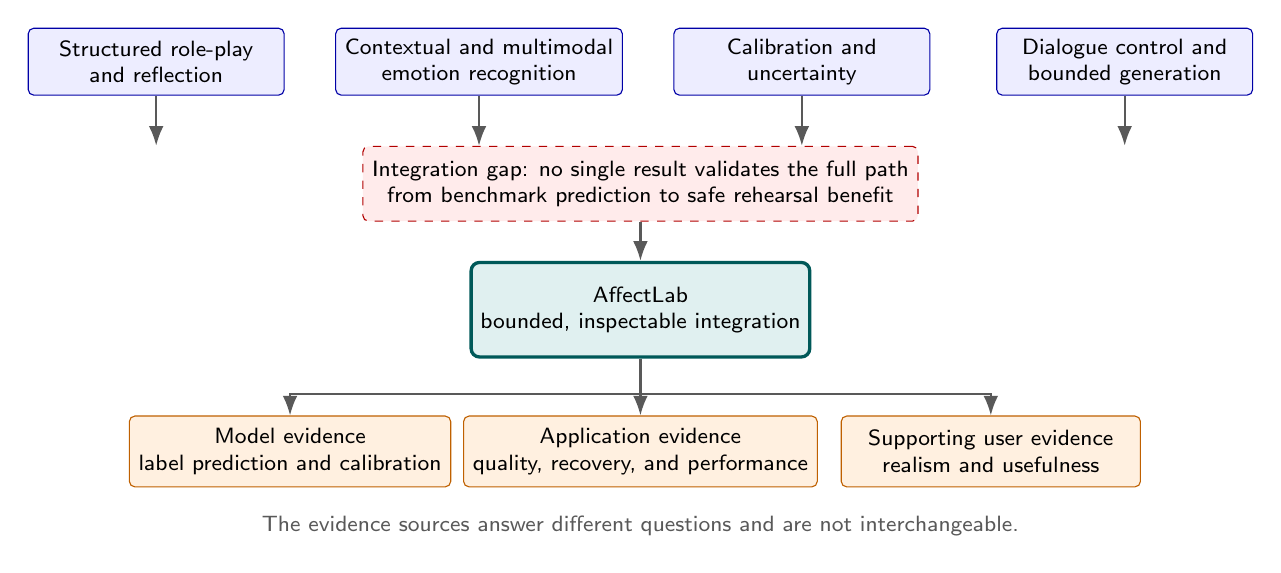
\begin{tikzpicture}[
    font=\sffamily\footnotesize,
    stream/.style={draw=blue!65!black, fill=blue!7, rounded corners=2pt,
        align=center, minimum width=3.25cm, minimum height=0.85cm},
    integration/.style={draw=teal!70!black, fill=teal!12, very thick,
        rounded corners=3pt, align=center, minimum width=4.2cm, minimum height=1.2cm},
    evidence/.style={draw=orange!75!black, fill=orange!12, rounded corners=2pt,
        align=center, minimum width=3.8cm, minimum height=0.9cm},
    gap/.style={draw=red!70!black, fill=red!8, dashed, rounded corners=2pt,
        align=center, minimum width=4.2cm, minimum height=0.95cm},
    flow/.style={-{Latex[length=2.5mm]}, thick, draw=black!65}
]
\node[stream] (practice) at (0,2.2) {Structured role-play\\and reflection};
\node[stream] (erc) at (4.1,2.2) {Contextual and multimodal\\emotion recognition};
\node[stream] (calibration) at (8.2,2.2) {Calibration and\\uncertainty};
\node[stream] (dialogue) at (12.3,2.2) {Dialogue control and\\bounded generation};

\node[gap] (gap) at (6.15,0.65) {Integration gap: no single result validates the full path\\from benchmark prediction to safe rehearsal benefit};
\node[integration] (affectlab) at (6.15,-0.95) {AffectLab\\bounded, inspectable integration};

\node[evidence] (model) at (1.7,-2.75) {Model evidence\\label prediction and calibration};
\node[evidence] (system) at (6.15,-2.75) {Application evidence\\quality, recovery, and performance};
\node[evidence] (human) at (10.6,-2.75) {Supporting user evidence\\realism and usefulness};

\foreach \source in {practice,erc,calibration,dialogue}
    \draw[flow] (\source.south) -- (gap.north -| \source.south);
\draw[flow] (gap) -- (affectlab);
\draw[flow] (affectlab.south) -- ++(0,-0.45) -| (model.north);
\draw[flow] (affectlab) -- (system);
\draw[flow] (affectlab.south) -- ++(0,-0.45) -| (human.north);

\node[align=center, text=black!65] at (6.15,-3.7)
    {The evidence sources answer different questions and are not interchangeable.};
\end{tikzpicture}
}
\caption{Relationship between the reviewed research streams, the AffectLab integration gap, and its complementary model, application, and supporting user evidence.}
\label{fig:literature-gap}
\end{figure}

\section{Research Gap and Positioning of AffectLab}\label{sec:sota-gap}

The identified research gap is not that conversational role-play, emotion recognition, multimodal fusion, or feedback generation have never been studied. Each has an extensive literature. Rather, the literature motivates a need for a carefully bounded, reproducibly evaluated integration in which (i) a live-compatible textual context model is compared with an utterance-only baseline; (ii) independent text and speech models are compared with a transparent fusion mechanism; (iii) classification performance is distinguished from calibrated operational confidence; and (iv) affect predictions are allowed to influence only explicit, low-consequence role-play actions. This is an \emph{integration and evaluation gap}, not a claim of universal novelty or proof that no similar application exists.

AffectLab addresses this gap through the following linked decisions. Its machine-learning study uses a four-category IEMOCAP task with five held-out sessions, a causal history window for text, an independent audio branch, and late fusion. Equal-weight and validation-fitted configurations are distinguished, and calibration is examined separately from classification. This is intended to provide controlled evidence for RQ1 and RQ2 without claiming real-world emotion understanding \cite{busso2008iemocap,li2022contextaware,guo2017calibration}.

Its conversational component uses scenario-specific, deterministic stages and completion rules, while optional language-model generation provides bounded linguistic variation. Confidence, agreement, modality availability, and the user's stated pacing preference are interpreted by a versioned, inspectable adaptation policy. Missing or disputed emotion evidence leads to baseline interaction or an explicit user choice rather than an imposed psychological interpretation. Safety and feedback are independent of the affect classifier, and generation failures have deterministic fallbacks. Together, these choices turn RQ3 into a question about verifiable application behaviour rather than an untestable claim of machine empathy \cite{bohus2009ravenclaw,lu2025roleplay,ovadia2019shift}.

Finally, AffectLab treats communication rehearsal as a useful, reflective activity delivered through a fully integrated application. Users practise workload negotiation, boundary maintenance, and the expression of relationship needs, then inspect evidence-linked feedback, repeat or branch an exchange, and record an actionable takeaway. RQ4 is therefore addressed through developer-led verification of the complete product across functional, persistence, recovery, accessibility, responsive-interface, performance, and deployment boundaries. A small pilot contributes supporting perceptions of realism and usefulness but is not asked to prove product readiness or causal communication improvement \cite{lee2020virtualpatients,lin2024imbue}.

\section{Chapter Summary}\label{sec:sota-summary}

Previous research provides substantial evidence for the value of structured communication practice, the usefulness of instructional feedback and reflection, the contribution of conversational context to emotion classification, the availability of strong pre-trained acoustic and textual representations, and the potential of multimodal fusion. It also reveals important limitations: benchmarks are domain-specific, labels do not directly measure private emotion, model confidence can be unreliable, generated dialogue can lose consistency, and apparently helpful simulations do not necessarily produce transferable learning \cite{lee2020virtualpatients,lin2024imbue,li2022contextaware,ovadia2019shift,lu2025roleplay}.

The work undertaken in this dissertation is consequently different from simply training another emotion classifier or constructing an unconstrained role-playing chatbot. AffectLab combines controlled context-aware text and speech experiments with a deliberately modest affect-adaptation policy, structured dialogue management, evidence-linked feedback, optional generation, reproducible fallbacks, and layered technical verification. Its contribution is to join these parts into a transparent, production-oriented application while keeping conclusions within the available evidence. Chapter~\ref{chap:proposed-system-architecture} defines the proposed architecture, requirements, scope, ethical boundaries, and limitations; Chapter~\ref{chap:implementation} documents the model and application implementation; and Chapter~\ref{chap5} presents the evaluation methodology and results.

\chapter{Proposed System Architecture}
\label{chap:proposed-system-architecture}

\section{System Overview}
\label{sec:system-overview}

AffectLab is designed as a hybrid, full-stack, production-oriented application for rehearsing difficult interpersonal conversations. Its architecture combines deterministic application logic, trained affect-recognition models, optional generative services, and a browser-based interaction interface. The system is not constructed as a single end-to-end conversational model. Instead, responsibilities are separated so that probabilistic components can contribute linguistic flexibility and affective information without controlling safety-critical or evaluative decisions.

The central architectural principle is the separation of \emph{inference}, \emph{control}, and \emph{presentation}. The affect-recognition subsystem estimates a distribution over a limited set of emotion categories from conversational text and optional speech. The dialogue-control subsystem determines how the scenario progresses, which communication features have been observed, and whether a completion condition has been reached. The response-generation subsystem expresses the selected dialogue action using either constrained generative wording or a deterministic template. The interface presents the conversation, optional affect information, feedback, and reflection tools to the user. This separation makes it possible to inspect and test each decision independently.

The system follows a text-first design. A user can complete the entire rehearsal by typing, while voice input is an optional enhancement. At the beginning of a rehearsal, the user selects a scenario, difficulty level, and, where available, a simulated character profile. The standard scenarios concern workload negotiation, personal boundary-setting, and the expression of a relationship need. Each scenario defines its objective, expected communication features, dialogue stages, difficulty-dependent behaviour, and possible completion outcomes.

During the rehearsal, the user submits a textual utterance and may optionally attach a short voice recording. The text is always available to the dialogue and safety components. When voice input and trained-model inference are enabled, the recording is processed for the current request and is not retained as part of the conversation history. Denial of microphone access, missing audio, or an inference failure therefore does not prevent the rehearsal from continuing.

Table~\ref{tab:architecture-components} summarises the main architectural components and the boundaries placed around their responsibilities.

Figure~\ref{fig:system-architecture} shows the corresponding information and authority flow. Solid paths represent the core workflow, while dashed paths identify optional evidence or services whose absence must not prevent text-based rehearsal.

\begin{figure}[htbp]
\centering
\resizebox{\textwidth}{!}{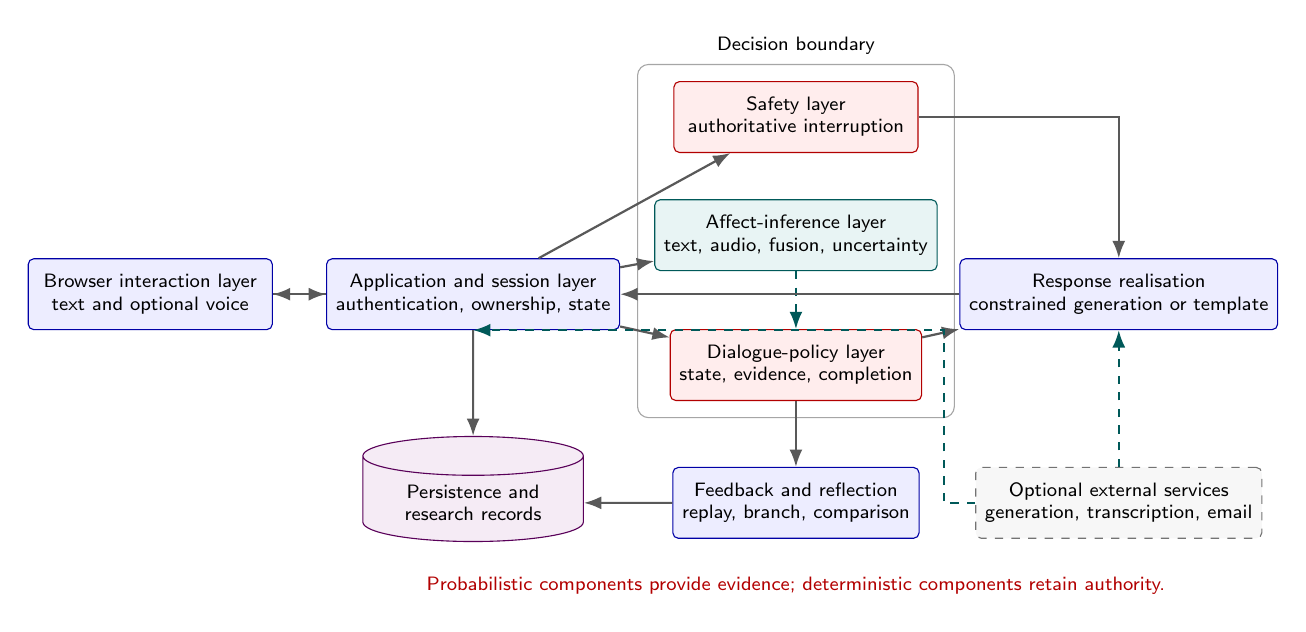
\begin{tikzpicture}[
    font=\sffamily\scriptsize,
    component/.style={draw=blue!65!black, fill=blue!7, rounded corners=2pt,
        align=center, minimum width=3.1cm, minimum height=0.9cm},
    authority/.style={draw=red!70!black, fill=red!7, rounded corners=2pt,
        align=center, minimum width=3.1cm, minimum height=0.9cm},
    evidence/.style={draw=teal!70!black, fill=teal!9, rounded corners=2pt,
        align=center, minimum width=3.1cm, minimum height=0.9cm},
    store/.style={cylinder, shape border rotate=90, aspect=0.25,
        draw=violet!70!black, fill=violet!8, align=center,
        minimum width=2.8cm, minimum height=1.05cm},
    optional/.style={draw=black!55, fill=black!3, dashed, rounded corners=2pt,
        align=center, minimum width=3.0cm, minimum height=0.9cm},
    flow/.style={-{Latex[length=2.2mm]}, thick, draw=black!65},
    signal/.style={-{Latex[length=2.2mm]}, thick, dashed, draw=teal!70!black}
]
\node[component] (ui) at (0,0) {Browser interaction layer\\text and optional voice};
\node[component] (app) at (4.1,0) {Application and session layer\\authentication, ownership, state};
\node[authority] (safety) at (8.2,2.25) {Safety layer\\authoritative interruption};
\node[evidence] (affect) at (8.2,0.75) {Affect-inference layer\\text, audio, fusion, uncertainty};
\node[authority] (policy) at (8.2,-0.9) {Dialogue-policy layer\\state, evidence, completion};
\node[component] (realise) at (12.3,0) {Response realisation\\constrained generation or template};
\node[component] (feedback) at (8.2,-2.65) {Feedback and reflection\\replay, branch, comparison};
\node[store] (store) at (4.1,-2.65) {Persistence and\\research records};
\node[optional] (external) at (12.3,-2.65) {Optional external services\\generation, transcription, email};

\draw[flow] (ui) -- (app);
\draw[flow] (app) -- (safety);
\draw[flow] (app) -- (affect);
\draw[flow] (app) -- (policy);
\draw[signal] (affect) -- (policy);
\draw[flow] (policy) -- (realise);
\draw[flow] (safety.east) -| (realise.north);
\draw[flow] (realise.west) -- ++(-0.45,0) |- (app.east);
\draw[flow] (app) -- (ui);
\draw[flow] (policy) -- (feedback);
\draw[flow] (feedback) -- (store);
\draw[flow] (app) -- (store);
\draw[signal] (external) -- (realise);
\draw[signal] (external.west) -- ++(-0.4,0) |- (app.south);

\begin{scope}[on background layer]
  \node[fit=(safety)(affect)(policy), draw=black!35, rounded corners=4pt,
      fill=white, inner sep=6pt, label={[font=\sffamily\scriptsize]above:Decision boundary}] {};
\end{scope}

\node[align=center, text=red!70!black] at (8.2,-3.7)
    {Probabilistic components provide evidence; deterministic components retain authority.};
\end{tikzpicture}
}
\caption{Logical architecture of AffectLab and separation between probabilistic evidence and authoritative application control.}
\label{fig:system-architecture}
\end{figure}

\begin{table}[htbp]
\centering
\caption{Principal components of the AffectLab architecture.}
\label{tab:architecture-components}
\footnotesize
\begingroup
\setlength{\tabcolsep}{4pt}
\begin{tabular}{|p{0.20\linewidth}|p{0.35\linewidth}|p{0.35\linewidth}|}
\hline
\textbf{Component} & \textbf{Primary responsibility} & \textbf{Architectural boundary} \\ \hline

Interaction layer &
Supports scenario selection, text and optional voice input, conversation display, pausing, replay, branching, feedback review, and personal takeaways. &
Does not determine dialogue outcomes, affect labels, safety decisions, or feedback scores. \\ \hline

Application and session layer &
Coordinates authenticated requests, session state, scenario configuration, conversation history, model calls, and persistence. &
Accepts decisions from specialised components but does not treat a generated response as the authoritative dialogue state. \\ \hline

Safety layer &
Examines textual input for crisis-related language and applies a predefined interruption response when required. &
Operates independently of affect classification and takes precedence over dialogue generation and affect adaptation. \\ \hline

Affect-inference layer &
Produces contextual text, audio, and fused probability distributions together with confidence, agreement, and availability information. &
Provides bounded evidence rather than a statement of the user's true emotional state. Its output cannot determine safety, scenario success, or feedback scores. \\ \hline

Dialogue-policy layer &
Detects observable communication features, advances the scenario state, selects the simulated character's intended action, and determines completion or unresolved outcomes. &
Uses explicit, scenario-specific rules. It is authoritative for progression even when generative response wording is enabled. \\ \hline

Response-realisation layer &
Transforms the dialogue action into a natural-language response using constrained generation or a deterministic template. &
May alter wording but cannot modify the selected action, completion state, recorded evidence, or safety response. \\ \hline

Feedback and reflection layer &
Calculates communication metrics, links them to supporting turns, and supports replay, retry, branch comparison, and takeaway creation. &
Bases assessment on recorded observable evidence. Generative phrasing cannot introduce unsupported findings. \\ \hline

Persistence and research layer &
Stores account-owned sessions, textual turns, dialogue decisions, feedback evidence, model provenance, and permitted research measures. &
Does not retain raw voice recordings and separates identifiable application data from pseudonymous research exports. \\ \hline
\end{tabular}
\endgroup
\end{table}

For each submitted utterance, processing begins with authentication, session-ownership validation, and input validation. The safety layer then examines the textual message before ordinary dialogue generation occurs. If a safety condition is detected, the normal role-play path is interrupted, a predefined safety response is returned, and the interruption is recorded. This ordering prevents optional affective or generative components from overriding an explicit safety decision.

When no safety interruption is required, the affective and conversational analyses are performed. The contextual text model receives the current message together with a causal window of preceding turns. If an audio sample is available, the audio model analyses the corresponding speech signal independently. The calibrated text and audio probability distributions can then be combined through late fusion. The system retains the individual modality outputs so that disagreement, missing information, and the contribution of each modality remain observable.

The resulting affective estimate is interpreted by a bounded adaptation policy. The policy considers model availability, calibrated confidence, agreement between modalities, the current dialogue state, and the user's selected pacing preference. Where affect adaptation is enabled and the evidence satisfies the declared conditions, the system may make a limited change such as adding a tentative acknowledgement. Low confidence or disagreement may lead to an explicit pacing choice, while unavailable inference produces the standard non-adaptive response. The policy does not describe the estimated category as a verified internal emotion.

In parallel with this bounded adaptation, the deterministic dialogue policy evaluates the user's message against the active scenario. It records observable language features and selects the next dialogue action. Depending on the scenario, relevant features may include a specific request, a concrete detail, an ``I'' statement, non-blaming language, acknowledgement of another perspective, maintenance of a boundary, or a proposed next step. The policy also determines whether the conversation should advance, continue under resistance, finish successfully, close without resolution, or stop because the maximum number of turns has been reached.

The selected action is passed to the response-realisation component. When generative services are enabled, a language model receives a constrained representation of the scenario, simulated character, difficulty, current state, and required dialogue action. The generated wording is accepted only as a realisation of that action. If generation is disabled, unavailable, or invalid, the system uses the deterministic response associated with the same action. Consequently, a service failure can reduce linguistic variety but does not remove the core rehearsal workflow.

After the response has been produced, the system persists the textual turns and their associated decision metadata. This metadata includes the dialogue state before and after the exchange, detected communication evidence, selected action, reason codes, affect-policy decision, model or policy versions, and whether generative or fallback wording was used. Recording these elements supports reproducibility and makes it possible to distinguish what the system decided from how that decision was expressed.

At the end of a rehearsal, the feedback component calculates scenario-specific metrics from the evidence accumulated during the conversation. Each metric is linked to the turn or turns that support it. Optional generative processing may improve the readability of the feedback, but the deterministic metrics and recorded evidence remain authoritative. The completed conversation can subsequently be replayed, retried from the latest exchange, or used as the basis for an alternative branch. Branch comparison evaluates the new continuation separately from the conversational context copied from the original attempt.

This architecture supports the research questions at distinct levels. The contextual text, audio, fusion, and calibration components support the model comparisons in RQ1 and RQ2. The separation between affect inference, bounded adaptation, deterministic dialogue control, and safety addresses RQ3. The integrated rehearsal, feedback, persistence, recovery, accessibility, and deployment workflow provides the system evaluated for application quality in RQ4. Maintaining these architectural boundaries also prevents model classification performance, policy conformance, application readiness, and supplementary user feedback from being treated as interchangeable forms of evidence.

\section{System Requirements and Scope}
\label{sec:system-requirements-scope}

\subsection{Overview}
\label{subsec:requirements-overview}

The system requirements translate the research aims introduced in Chapter~\ref{chap1} and the design implications identified in Chapter~\ref{chap2} into explicit capabilities and constraints for AffectLab. They define what the application is expected to do, the conditions under which it should operate, and the responsibilities that must remain outside probabilistic affect recognition and generative artificial intelligence.

The requirements are divided into functional and non-functional requirements. Functional requirements describe user-visible capabilities and internal system behaviours. Non-functional requirements describe qualities that apply across those capabilities, including safety, privacy, explainability, reliability, accessibility, and reproducibility. Together, they provide a basis for designing the architecture and for evaluating whether the implemented system conforms to its intended behaviour.

A distinction is maintained between \emph{core} and \emph{optional} functions. Text-based structured rehearsal, deterministic dialogue control, safety handling, feedback, and session management constitute the core workflow. Voice capture, trained multimodal inference, transcription, generative response wording, and generative feedback phrasing are optional enhancements. The absence or failure of an optional component must not make the core rehearsal unusable.

\subsection{Scope of the System}
\label{subsec:system-scope}

AffectLab is intended to support adults who wish to prepare for and rehearse ordinary but potentially difficult interpersonal conversations. It provides a private, repeatable environment in which users can practise alternative wording, experience controlled conversational resistance, inspect feedback linked to their own messages, and reflect on possible next steps.

The primary scope comprises three standard communication situations:

\begin{itemize}
    \item negotiating workload or priorities with a manager;
    \item stating and maintaining a personal boundary; and
    \item expressing a relationship need using specific and non-blaming language.
\end{itemize}

Each standard scenario defines a simulated character, a communication objective, expected observable features, dialogue stages, difficulty-dependent behaviour, and explicit completion conditions. The system may additionally support user-prepared scenarios, provided that they use the communication features and safety constraints supported by the application.

The system supports text-based interaction as the default modality. Optional voice input can be used for transcription and acoustic affect analysis when the relevant services are enabled. Affect analysis is limited to estimates over predefined categories derived from the selected research dataset. These estimates may inform restrained changes in conversational pacing, but they are not presented as direct measurements of the user's internal emotional state.

The scope also includes post-rehearsal reflection. Users can inspect evidence-grounded feedback, replay an attempt, retry an exchange, create an alternative conversational branch, compare compatible attempts, record a personal takeaway, and prepare an action card. These functions support deliberate practice rather than unrestricted social conversation.

For optional research use, AffectLab includes versioned consent and eligibility procedures, pre- and post-rehearsal measures, pseudonymous research records, technical-event recording, and restricted aggregate export. These functions support supplementary study workflows. They do not transform the application into a clinical intervention or establish that practice transfers to real-world behaviour.

\subsection{Functional Requirements}
\label{subsec:functional-requirements}

The functional requirements of AffectLab are as follows.

\begin{description}

    \item[\textbf{FR1. User authentication and ownership}]  
    The system shall provide account-based access and shall associate every conversation, rehearsal, feedback record, branch, preparation record, and personal takeaway with its owning user. A user shall not be able to access another user's resources.

    \item[\textbf{FR2. Onboarding and disclosure}]  
    The system shall explain its purpose, limitations, data handling, optional use of voice, and non-clinical status before the user begins the main workflow. It shall not present itself as a therapist, diagnostic instrument, mediator, or emergency service.

    \item[\textbf{FR3. User preferences and practice goals}]  
    The system shall allow users to select and update practice goals and relevant interaction preferences. Optional microphone use and affect adaptation shall remain under user control.

    \item[\textbf{FR4. Scenario preparation}]  
    The system shall allow the user to prepare for a conversation by recording its context, the intended outcome, relevant concerns, and a possible objection or source of resistance. Preparation information shall be available to the corresponding rehearsal without becoming an authoritative assessment of the situation.

    \item[\textbf{FR5. Scenario selection}]  
    The system shall provide standard scenarios for workload negotiation, personal boundary-setting, and expressing a relationship need. It may also allow account-owned custom scenarios constructed from the supported communication objectives and observable features.

    \item[\textbf{FR6. Difficulty and character configuration}]  
    The system shall support multiple difficulty levels and character profiles. These settings may vary cooperation, resistance, scepticism, time pressure, or willingness to clarify, but shall not modify the safety rules or the meaning of the scenario's communication objectives.

    \item[\textbf{FR7. Rehearsal lifecycle}]  
    The user shall be able to start, pause, resume, manually finish, and leave a rehearsal. The system shall preserve the current state when continuation is permitted and shall record the reason for completion or interruption.

    \item[\textbf{FR8. Text-first interaction}]  
    The system shall accept a textual message for each conversational turn. All core scenario, safety, feedback, and reflection functions shall remain available without microphone access or audio input.

    \item[\textbf{FR9. Optional voice input}]  
    Where voice functions are enabled, the system shall allow the user to record a short audio sample. A transcript produced from the recording shall be presented for review and editing before it is submitted as a conversational turn.

    \item[\textbf{FR10. Safety precedence}]  
    The system shall examine textual input for supported crisis-related indicators before applying ordinary affect adaptation or response generation. When a safety condition is detected, it shall interrupt the ordinary role-play path, return the predefined safety response, and record the rehearsal as safety-interrupted.

    \item[\textbf{FR11. Contextual text inference}]  
    Where trained inference is enabled, the system shall construct the text-model input from the current utterance and a fixed causal window of preceding conversational turns. It shall not use future dialogue turns or unavailable annotation information.

    \item[\textbf{FR12. Acoustic inference and multimodal fusion}]  
    When valid audio is supplied, the system shall produce separate textual and acoustic probability distributions and may combine them using the declared late-fusion configuration. It shall retain modality availability, confidence, agreement, calibration, and model-version information needed to interpret the result.

    \item[\textbf{FR13. Missing-modality handling}]  
    The system shall handle missing, rejected, invalid, or failed audio without terminating the text-based rehearsal. The absence of audio shall not be interpreted as negative evidence about the user's affect.

    \item[\textbf{FR14. Bounded affect adaptation}]  
    Where affect adaptation is enabled and permitted, the system shall translate model confidence, modality agreement, inference availability, user preference, and dialogue state into a limited set of predefined actions. Affect predictions shall not determine crisis handling, scenario success, feedback scores, participant eligibility, or research inclusion.

    \item[\textbf{FR15. Deterministic dialogue progression}]  
    The system shall use scenario-specific policies to detect observable communication features, update the dialogue stage, select the simulated character's intended action, and determine whether a completion condition has been reached.

    \item[\textbf{FR16. Evidence recording}]  
    For every relevant user turn, the system shall record the observable features detected by the active scenario policy and link those features to the corresponding conversation turn. The system shall preserve the policy and scoring versions used to produce the evidence.

    \item[\textbf{FR17. Constrained response realisation}]  
    The system shall transform the selected dialogue action into a simulated-character response. A configured language model may phrase the response, but it shall not alter the authoritative dialogue action, completion decision, safety result, or recorded evidence.

    \item[\textbf{FR18. Deterministic fallback}]  
    If generative response production is disabled, unavailable, rejected, times out, or produces an invalid result, the system shall return a deterministic response associated with the same dialogue action. The source of the response and any fallback reason shall be recorded.

    \item[\textbf{FR19. Explicit rehearsal outcomes}]  
    The system shall distinguish between relevant completion outcomes, including achievement of a practical next step, maintenance of a boundary, unresolved closure, manual completion, maximum-turn completion, and safety interruption. Scenario success shall not always require agreement from the simulated character.

    \item[\textbf{FR20. Evidence-grounded feedback}]  
    At the end of a rehearsal, the system shall calculate scenario-specific communication metrics from recorded evidence. Feedback shall identify supported strengths and areas for further practice without making claims about personality, diagnosis, or general communication competence.

    \item[\textbf{FR21. Controlled feedback phrasing}]  
    A language model may improve the wording of deterministic feedback when configured, but it shall not introduce a strength, weakness, score, or supporting example that is absent from the authoritative feedback record.

    \item[\textbf{FR22. Replay and evidence inspection}]  
    The system shall allow the user to review the completed conversation and identify the turns associated with feedback evidence, dialogue decisions, and permitted affect-adaptation actions.

    \item[\textbf{FR23. Retry and branching}]  
    The system shall support retrying an eligible exchange and creating an alternative branch from a supported point in the conversation. Branching shall preserve the copied context while distinguishing it from newly generated continuation turns.

    \item[\textbf{FR24. Attempt comparison}]  
    The system shall allow comparison only between compatible attempts, such as rehearsals using the same scenario and scoring version. For a branch, feedback shall evaluate the new continuation separately from the copied context.

    \item[\textbf{FR25. Personal reflection}]  
    The system shall allow the user to save a personal takeaway and create an action-oriented summary of wording or next steps they wish to remember. User-authored reflections shall remain distinct from system-generated feedback.

    \item[\textbf{FR26. Session persistence and deletion}]  
    The system shall retain the textual and structural information required for session recovery, replay, branching, and feedback for the configured retention period. Users shall be able to delete eligible sessions and their account-owned data.

    \item[\textbf{FR27. Research participation controls}]  
    When the research workflow is enabled, the system shall record versioned consent, eligibility confirmation, questionnaire status, required-task progress, and withdrawal. Research collection shall begin only after the applicable consent and eligibility requirements have been satisfied.

    \item[\textbf{FR28. Pseudonymous research access}]  
    The system shall provide authorised researchers with aggregate monitoring and pseudonymous exports containing only the fields required by the study protocol. Research exports shall exclude names, email addresses, passwords, raw conversation text, raw audio, custom scenario wording, feedback prose, and personal takeaways.

\end{description}

\subsection{Non-Functional Requirements}
\label{subsec:non-functional-requirements}

The non-functional requirements apply across the complete system.

\begin{description}

    \item[\textbf{NFR1. Safety}]  
    Safety handling shall remain independent of the trained affect classifier and shall take precedence over affect adaptation and generative response production. Failure of a probabilistic component shall not suppress a deterministic safety response.

    \item[\textbf{NFR2. Graceful degradation}]  
    The core text-based rehearsal shall remain operational when microphone permission is denied, audio is unavailable, trained inference cannot be loaded, transcription fails, or an external generative service is disabled or unreachable.

    \item[\textbf{NFR3. User control}]  
    Users shall be able to decline optional voice processing, disable eligible adaptation, select an available pacing preference, pause a rehearsal, finish it manually, or leave it without being required to accept an inferred emotional interpretation.

    \item[\textbf{NFR4. Privacy and data minimisation}]  
    The system shall collect and retain only information required for the declared application and research functions. Raw audio shall be processed transiently and shall not be stored as part of the conversation record.

    \item[\textbf{NFR5. Security}]  
    The system shall protect accounts and sessions through secure password storage, authenticated access, resource-ownership checks, restricted configuration secrets, session expiry, and deployment-appropriate transport and host controls.

    \item[\textbf{NFR6. Explainability and auditability}]  
    Consequential system behaviour shall be traceable to an explicit policy, evidence record, reason code, configuration, or safety rule. The system shall distinguish model predictions, dialogue decisions, generated wording, fallback responses, and feedback metrics.

    \item[\textbf{NFR7. Reproducibility}]  
    Model, policy, scenario, scoring, consent, study-protocol, and export-schema versions shall be recorded where they affect interpretation. Evaluation configurations shall be preserved so that reported results can be reproduced without selecting settings from final test outcomes.

    \item[\textbf{NFR8. Reliability and consistency}]  
    Repeated execution with the same deterministic state and input shall produce the same dialogue transition, completion decision, evidence record, and feedback score. Concurrent or duplicate submissions shall not silently produce contradictory session states.

    \item[\textbf{NFR9. Responsiveness and failure recovery}]  
    Model-dependent operations shall use bounded execution and expose appropriate busy, error, or fallback states. Failure of an optional operation shall return control to the user rather than leaving the session in an indeterminate state. The locally controlled text-first path shall be measurable independently of provider and model latency so that responsiveness regressions can be detected reproducibly.

    \item[\textbf{NFR10. Accessibility}]  
    Core workflows shall support keyboard navigation, visible focus, accessible form labels, understandable status announcements, sufficient contrast, reduced-motion preferences, and layouts suitable for desktop and mobile interaction.

    \item[\textbf{NFR11. Maintainability and modularity}]  
    Persistence, affect inference, dialogue policy, safety, generation, feedback, and research-data functions shall be separated through explicit interfaces. It shall be possible to replace an optional model or external provider without rewriting the authoritative scenario logic.

    \item[\textbf{NFR12. Testability}]  
    The architecture shall permit automated tests of dialogue transitions, safety precedence, affect-policy decisions, missing-modality behaviour, fallback generation, feedback evidence, access control, persistence, replay, branching, and research export.

    \item[\textbf{NFR13. Data integrity}]  
    Stored sessions shall preserve the relationship between turns, dialogue decisions, evidence, feedback, branches, and version information. Invalid or stale updates shall be rejected rather than silently overwriting newer session state.

    \item[\textbf{NFR14. Appropriate presentation of uncertainty}]  
    Affect outputs shall be presented as model estimates rather than verified facts. Low-confidence, conflicting, or unavailable results shall be distinguishable from supported predictions and shall not be converted into stronger psychological claims.

\end{description}

\subsection{Assumptions}
\label{subsec:system-assumptions}

The proposed architecture is based on the following assumptions:

\begin{itemize}
    \item Users are adults practising ordinary interpersonal communication rather than seeking diagnosis, treatment, crisis intervention, or professional mediation.
    
    \item The primary interaction language is English because the scenarios, deterministic language features, safety phrases, and emotion-recognition datasets are designed for English-language input.
    
    \item Every conversational turn contains text, either typed directly or reviewed after optional transcription. The system does not rely exclusively on acoustic input.
    
    \item Users have access to a modern web browser and a sufficiently stable connection to the application. Voice functions additionally require a compatible microphone and browser permission.
    
    \item The predefined communication features are limited proxies for observable wording. Their detection does not provide a complete assessment of communication quality or interpersonal effectiveness.
    
    \item Predictions derived from IEMOCAP may not generalise to spontaneous speech, different languages, cultures, accents, devices, or recording environments. Calibration measured on the benchmark may also deteriorate under deployment conditions.
    
    \item Agreement between textual and acoustic models increases the consistency of available model evidence but does not prove that the predicted category is correct.
    
    \item Optional external services are available only when valid configuration and credentials are provided. Their outputs, availability, latency, and data-handling conditions are not fully controlled by AffectLab.
    
    \item Replay, feedback, and branching require the system to retain conversation text for a declared period. Users are expected to receive clear information about this retention before using the application.
    
    \item Any participant study or remote deployment will occur only after the required institutional, ethical, security, and data-protection reviews have been completed.
\end{itemize}

\subsection{System Boundaries}
\label{subsec:system-boundaries}

The system boundaries define both the technical responsibility of AffectLab and the limits of the claims that may be made from its outputs.

\begin{table}[htbp]
\centering
\caption{Principal boundaries of the proposed AffectLab system.}
\label{tab:system-boundaries}
\footnotesize
\begingroup
\setlength{\tabcolsep}{4pt}
\begin{tabular}{|p{0.19\linewidth}|p{0.34\linewidth}|p{0.37\linewidth}|}
\hline
\textbf{Boundary} & \textbf{Within the system} & \textbf{Outside the system} \\ \hline

Intended use &
Preparation, structured rehearsal, evidence-grounded feedback, repetition, and reflection for difficult interpersonal conversations. &
Therapy, diagnosis, clinical treatment, emergency response, professional mediation, employment assessment, or institutional surveillance. \\ \hline

Affect recognition &
Prediction of predefined dataset labels from causal text context and optional speech, including confidence and modality agreement. &
Direct measurement of private emotion, intention, truthfulness, personality, mental health, or future behaviour. \\ \hline

Dialogue control &
Scenario-specific stages, resistance, observable features, response actions, completion rules, and deterministic fallbacks. &
Unrestricted open-domain conversation or autonomous alteration of learning objectives by a language model. \\ \hline

Generative artificial intelligence &
Optional wording of an already selected response action and optional phrasing of evidence-grounded feedback. &
Authority over safety, scenario progression, success, scoring, eligibility, research outcomes, or unsupported advice. \\ \hline

Safety &
Conservative text-first checks, interruption of the rehearsal, predefined guidance, and separation from affect inference. &
Comprehensive crisis detection, clinical risk assessment, monitoring of the user's environment, or contact with emergency services. \\ \hline

Data handling &
Authenticated session storage, limited conversation retention, transient audio processing, account controls, and pseudonymous research records. &
Guarantees about infrastructure or external-provider processing beyond the configured deployment and applicable agreements. \\ \hline

Evaluation &
Emotion-classification evaluation, calibration analysis, engineering conformance, accessibility, recovery, and performance tests, with a small supplementary user pilot. &
Proof of therapeutic effectiveness, causal learning benefit, reliable real-world emotion understanding, or transfer to future conversations. \\ \hline
\end{tabular}
\endgroup
\end{table}

External systems may include the user's browser and microphone, an email delivery service, an optional transcription or language-model provider, the database service, and the deployment infrastructure. AffectLab controls the information sent through its defined interfaces but cannot guarantee the internal availability, behaviour, or data-processing practices of an independently operated provider. Consequently, externally dependent functions must remain optional or provide an explicit failure path.

The system boundary also separates participant-facing data from research-facing data. Participants may access their conversation content, feedback, branches, and takeaways. Researchers receive only the pseudonymous measures authorised by the study protocol. Operational access to a deployed database or server is an administrative responsibility and is not equivalent to permission to use participant data for research.

\subsection{Summary}
\label{subsec:requirements-summary}

AffectLab is scoped as a text-first, structured communication-rehearsal application with optional voice, affective, generative, and research-support capabilities. Its functional requirements cover the complete path from onboarding and scenario preparation to controlled role-play, multimodal inference, feedback, replay, branching, reflection, and optional research-data collection. Its non-functional requirements emphasise safety precedence, graceful degradation, privacy, security, accessibility, explainability, reproducibility, responsiveness, and user control.

The defining constraint is that probabilistic components provide bounded support rather than authoritative control. Emotion predictions cannot determine safety, success, or assessment, while generative models cannot change dialogue decisions or invent feedback evidence. These requirements establish the basis for the component architecture and interaction flow described in the following sections.

\section{Ethical Considerations and Limitations}
\label{sec:ethical-considerations-limitations}

\subsection{Ethical Approach and Intended Use}
\label{subsec:ethical-approach}

AffectLab operates in a sensitive domain because users may enter personal information, discuss conflict, provide voice recordings, and receive system-generated interpretations or feedback. Ethical considerations are therefore treated as architectural requirements rather than as matters to be addressed only after implementation. The principal concerns are the possible misinterpretation of affect predictions, inappropriate reliance on generated responses, loss of user autonomy, exposure of sensitive information, unequal model performance, and confusion between communication rehearsal and psychological support.

The intended use of AffectLab is limited to voluntary preparation for and rehearsal of ordinary interpersonal conversations by adults. It is not intended for diagnosis, treatment, clinical triage, crisis monitoring, employment assessment, educational assessment, surveillance, deception, or the evaluation of another person without their knowledge. It must not be used to infer protected characteristics, stable personality traits, truthfulness, or psychological disorders.

The system is intended to support reflection rather than prescribe a correct way to conduct a relationship or workplace conversation. Its scenarios simplify complex interpersonal situations into structured practice tasks. Completing a scenario therefore means satisfying the declared communication conditions within the simulation; it does not establish that the same response is appropriate in every real-world context.

\subsection{Ethical Use of Affect Recognition}
\label{subsec:ethical-affect-recognition}

The most significant ethical risk associated with AffectLab is that a predicted emotion could be mistaken for knowledge of the user's internal state. The trained models do not directly observe emotion. They classify textual and acoustic patterns according to categories derived from annotations in IEMOCAP. These categories represent an operational benchmark rather than a complete theory of human affect \cite{busso2008iemocap}.

The primary four-class task contains anger, happiness, neutrality, and sadness, with excitement incorporated into the happiness category. It does not adequately represent anxiety, frustration, embarrassment, fear, shame, mixed affect, deliberate emotional masking, or uncertainty. A model can consequently be statistically correct according to the benchmark while still producing a description that is inappropriate for an individual user.

To reduce this risk, affect outputs are treated as uncertain evidence rather than facts. The interface and dialogue policy must avoid statements such as ``you are angry'' or ``the system knows that you are sad''. Where an affective response is permitted, the wording should remain tentative and should not require the user to accept the interpretation. The user may continue normally, select a preferred pace, or disable an eligible adaptive function.

Confidence does not eliminate this ethical concern. Neural classifiers may produce high-confidence errors, particularly when deployment data differ from their training distribution \cite{guo2017calibration,ovadia2019shift}. Similarly, agreement between the textual and acoustic models does not prove correctness because both may respond to the same misleading cue. The low-confidence threshold and agreement rules used by AffectLab are therefore operational safeguards rather than scientifically validated boundaries between correct and incorrect emotional interpretation.

The architecture restricts affect predictions to low-consequence and reversible actions. They cannot determine crisis escalation, scenario success, communication-skill scores, study eligibility, or research inclusion. If prediction is unavailable, uncertain, or conflicting, the system returns to baseline dialogue or offers an explicit user choice. This limits the harm that can result from an incorrect classification.

\subsection{User Autonomy, Transparency, and Avoidance of Dependency}
\label{subsec:autonomy-transparency}

Users should understand when they are interacting with deterministic application logic, a trained classifier, or a generative model. AffectLab therefore distinguishes dialogue decisions from their linguistic realisation and records whether a response was generated or produced from a deterministic template. Feedback metrics are similarly separated from any optional generative phrasing.

Voice input is optional and requires an explicit user action. A transcript created from a recording is placed in the message composer for review and editing rather than being submitted automatically. This allows the user to correct transcription errors and decide whether the content should become part of the conversation.

The user retains the ability to pause, resume, finish, or leave a rehearsal. Affect adaptation must not be used to pressure the user into continuing, accepting an interpretation, disclosing more information, or selecting a particular response. Manual completion is not treated as misconduct, and a user is not penalised for refusing voice input or declining an adaptive feature.

The system must also avoid encouraging emotional dependency. Generated language should not imply consciousness, exclusive understanding, personal attachment, or an ability to replace human relationships and professional services. AffectLab may support rehearsal and reflection, but it must not position itself as the user's primary source of emotional support or claim authority over consequential interpersonal decisions.

\subsection{Safety and Non-Clinical Boundaries}
\label{subsec:safety-boundaries}

Difficult-conversation practice may elicit or contain language associated with distress, self-harm, abuse, or immediate danger. AffectLab is not designed to assess the severity of such circumstances. Its safety mechanism is a conservative text-first interruption layer whose purpose is to prevent ordinary role-play from continuing when supported crisis-related expressions are detected.

Safety handling remains independent of multimodal affect inference. A four-category emotion classifier is not an appropriate crisis detector, and an apparently neutral prediction must not override explicit crisis-related language. Safety handling also takes precedence over the language model so that a generated response cannot suppress or replace the predefined interruption.

The safety layer nevertheless has important limitations. Lexical matching may fail when risk is expressed indirectly, metaphorically, sarcastically, with spelling variation, or in an unsupported language. Optional provider moderation may identify additional cases, but it is also probabilistic and cannot guarantee detection. Conversely, conservative rules may interrupt a conversation when crisis-related wording is quoted or discussed hypothetically.

The application is not continuously monitored, does not establish the user's physical location, and cannot independently contact emergency services or another trusted person. Its safety response can provide appropriate signposting, but it cannot perform clinical triage. These limitations must be disclosed before use and repeated when a safety interruption occurs. The risks of presenting generative wellness systems as substitutes for professional care further support this restrained scope \cite{defreitas2024wellness}.

\subsection{Privacy, Data Protection, and Data Governance}
\label{subsec:privacy-data-governance}

Conversation text may contain names, workplace details, relationship information, and other sensitive personal content. Voice recordings may additionally reveal identity-related characteristics, accent, health information, background conversation, or environmental details. The fact that users choose to enter this information does not remove the system's responsibility to minimise its collection and exposure.

The design follows the principles of purpose limitation, data minimisation, storage limitation, transparency, integrity, and confidentiality described by the General Data Protection Regulation \cite{eu2016gdpr}. These principles are reflected in several architectural decisions:

\begin{itemize}
    \item text is collected only when required for conversation, feedback, replay, or authorised research functions;
    \item microphone access requires an explicit user action;
    \item audio duration and accepted file size are restricted;
    \item raw audio is processed transiently and is not intentionally retained in the conversation record;
    \item account-owned conversations expire according to a declared retention policy;
    \item users can delete individual sessions and request account deletion;
    \item research records exclude raw conversation text, audio, custom scenario wording, feedback prose, and personal takeaways; and
    \item access to participant and researcher functions is separated and authenticated.
\end{itemize}

Pseudonymisation reduces direct identifiability but does not make active research records anonymous while they remain linkable for withdrawal or data management. This distinction must be explained accurately. Participants may withdraw from research and have identifiable study records removed where possible. If data have already been irreversibly de-identified and included in a frozen aggregate dataset, removal may no longer be technically possible; this limitation must be stated before consent rather than introduced only after withdrawal.

Research consent and the lawful basis for processing personal data are related but distinct matters. Participation consent should describe the study, its risks, voluntary nature, and withdrawal procedure. The data controller must separately determine and document the appropriate legal basis for each processing purpose. The existence of a consent screen alone does not demonstrate full data-protection compliance.

When an external provider is configured for transcription, generation, feedback phrasing, or moderation, relevant content may leave the locally controlled application boundary. Users must be told which functions involve external processing and whether a text-only or offline alternative is available. Provider credentials must remain outside source code and logs, while ordinary application logs should avoid storing prompts, generated responses, access tokens, or raw audio.

Technical controls such as password hashing, authenticated ownership checks, restricted research exports, transport encryption, secure configuration, rate limiting, and backup protection reduce risk but cannot guarantee absolute confidentiality. A remote pilot additionally requires deployment-specific security review, appropriate institutional approval, an assessed lawful basis, and consideration of whether a data-protection impact assessment is necessary.

\subsection{Fairness, Representation, and Accessibility}
\label{subsec:fairness-representation}

IEMOCAP contains a small number of English-speaking actors recorded in controlled dyadic sessions. Speaker-independent evaluation prevents direct reuse of test speakers during training, but it does not demonstrate equitable performance across cultures, accents, age groups, disabilities, gender identities, socioeconomic backgrounds, communication styles, recording devices, or spontaneous emotional situations \cite{busso2008iemocap}.

The available dataset is insufficient for strong demographic fairness conclusions. Reporting only aggregate accuracy could conceal systematically weaker behaviour for particular classes or speakers. The model evaluation should therefore include per-class results, confusion matrices, fold-level variation, and failure analysis. These analyses reveal some forms of uneven performance, but they do not establish demographic fairness when the required demographic coverage and statistical power are absent.

Bias can also arise from deterministic rules. Feature detectors may favour direct, standardised English phrasing and fail to recognise indirect requests, culturally specific politeness, neurodivergent communication patterns, quoted speech, or valid paraphrases. The detected features are therefore proxies for the scenario's declared objectives rather than universal measures of respectful or effective communication.

The system should not penalise a user for an accent, unavailable microphone, transcription error, disability, or preference for text. Core interaction must remain keyboard accessible and usable without audio. Accessible labels, visible focus, status announcements, reduced-motion support, and responsive layouts are required to reduce avoidable participation barriers. Nevertheless, compliance checks cannot establish accessibility for every user, and evaluation with diverse participants remains necessary.

\subsection{Generative Artificial Intelligence and Feedback Integrity}
\label{subsec:generative-ethics}

A generative model may produce fluent language while failing to follow the intended scenario. It may become overly agreeable, reinforce an unrealistic assumption, introduce unsupported content, or express advice with excessive confidence. Multi-turn role-play can also lose consistency as the conversation grows \cite{lu2025roleplay}. Natural wording must therefore not be interpreted as evidence that the response is educationally valid or emotionally accurate.

AffectLab limits the authority of generation by requiring the deterministic dialogue policy to select the response action first. The generator may express that action in varied language, but it cannot determine scenario completion, change the evidence record, or override safety. When generation is unavailable or rejected, the associated template response is used.

The same separation applies to feedback. Observable features and scores are computed deterministically. A generative model may phrase strengths and suggestions only from this structured record. It must not create a supporting example, skill observation, or criticism that is absent from the recorded evidence.

These safeguards reduce but do not eliminate generative risk. Prompt constraints cannot guarantee that every output is appropriate, culturally sensitive, or factually correct. Provider models and policies may also change after deployment. Generation source, model configuration, validation outcome, and fallback reason should consequently be retained as operational provenance.

\subsection{Research Ethics and Participant Protection}
\label{subsec:research-ethics}

The participant evaluation is designed as a feasibility and usability pilot rather than an effectiveness trial. Participation is restricted to adults who can understand the English-language information and provide informed consent. Individuals seeking crisis care, diagnosis, treatment, or emergency support are outside the intended study population. Eligibility confirmation is self-reported and must not be described as a clinical screening assessment.

Before participation, users must receive understandable information about:

\begin{itemize}
    \item the research purpose and study procedure;
    \item the non-clinical status of the system;
    \item the use and limitations of affect recognition;
    \item optional voice and external-provider processing;
    \item the information collected and its retention period;
    \item foreseeable privacy, emotional, and technical risks;
    \item the voluntary nature of participation;
    \item the right to pause, omit optional input, stop, or withdraw; and
    \item the circumstances under which withdrawn or irreversibly de-identified data can no longer be removed.
\end{itemize}

Required research tasks use standardised scenarios and intermediate difficulty to reduce unnecessary variation. Optional voice and multimodal affect inference are exploratory and are not required for study completion. Safety interruptions and technical failures are recorded as feasibility outcomes and must not be interpreted as communication-skill failures.

Pre- and post-rehearsal ratings are study-specific feasibility measures rather than validated clinical instruments. Participants may answer or explicitly skip them. Missing values must remain missing rather than being replaced with fabricated neutral scores. Research exports use pseudonymous identifiers and exclude conversation content. Only authorised researchers should access the research dashboard and exports.

Recruitment must not begin until the applicable institutional ethics approval, participant-facing materials, researcher contact details, retention schedule, deployment review, and data-management responsibilities have been confirmed. Material changes after recruitment begins require a new protocol version and, where applicable, renewed approval and participant consent.

\subsection{Legal and Regulatory Context}
\label{subsec:legal-regulatory-context}

The ethical safeguards described above do not by themselves establish legal compliance. Applicable obligations depend on the purpose of processing, the data used, the deployment context, the organisations involved, and the jurisdiction in which the system operates.

The European Union Artificial Intelligence Act prohibits certain emotion-inference uses in workplace and educational-institution contexts, subject to its stated exceptions \cite{eu2024aiact}. AffectLab is designed for voluntary individual rehearsal and not for employers, teachers, or institutions to assess workers or students. No employer or educational authority should receive individual affect predictions or use them for selection, discipline, grading, access, or performance evaluation. However, describing the application as voluntary research does not automatically determine its legal classification. The applicability of the prohibition and other obligations requires formal assessment before institutional or public deployment.

The AI Act does not replace the General Data Protection Regulation. Conversation text, account information, research measurements, and voice recordings may constitute personal data even where an AI Act prohibition does not apply. Whether a particular voice-processing operation involves special-category biometric data depends on how and why the data are processed and should not be assumed solely from the presence of an audio recording. Applicable lawful bases, transparency duties, data-subject rights, processor agreements, international transfers, retention rules, security measures, and impact-assessment obligations require deployment-specific review \cite{eu2016gdpr}.

Accordingly, the dissertation evaluates technical and ethical safeguards but does not claim to provide a definitive legal determination or compliance certification.

\subsection{Limitations of the Proposed System}
\label{subsec:proposed-system-limitations}

\subsubsection{Construct and model limitations}

AffectLab predicts benchmark categories rather than directly measuring emotion. Its labels simplify affective experience, and its confidence values are conditional on the model, dataset, and calibration procedure. Even a well-calibrated classifier can be wrong for an individual example. Performance on IEMOCAP does not demonstrate equivalent performance during real application use.

The contextual model uses a fixed number of preceding turns and cannot represent every relevant feature of a relationship or situation. The audio model may be influenced by microphone quality, background noise, speaking style, health, accent, or recording distance. Late fusion cannot correct an error when both modalities are misleading, and it may perform worse than the stronger individual modality when one input is degraded.

\subsubsection{Dialogue and feedback limitations}

Deterministic policies improve predictability but can respond only to anticipated stages and detectable language patterns. They may fail to recognise a valid paraphrase, sarcasm, indirect communication, or a creative solution. Template responses may become repetitive, while generated responses remain probabilistic despite their constraints.

Feedback metrics capture only the observable features defined for each scenario. They cannot evaluate sincerity, appropriateness for the user's actual relationship, non-verbal behaviour, long-term consequences, or the other person's interpretation. Users may also learn to optimise their wording for the detectors without developing a broader communication skill.

\subsubsection{Safety limitations}

The safety layer cannot identify every dangerous or abusive situation. It is strongest for explicit supported English phrases and weaker for indirect, coded, multilingual, or context-dependent expressions. It cannot verify whether a user is currently safe, determine their location, or provide a monitored emergency response. False positives and false negatives remain possible.

\subsubsection{Privacy and security limitations}

Although raw audio is not intentionally retained, transient processing and transmission still create exposure. Stored conversation text may contain sensitive information, and pseudonymous research data may remain linkable while withdrawal is supported. Software controls cannot eliminate risks arising from compromised devices, incorrect deployment configuration, administrator access, provider-side processing, unpatched dependencies, or unauthorised disclosure.

\subsubsection{Evaluation limitations}

The engineering tests use authored and synthetic cases. Passing them demonstrates conformance to declared policies but not performance across the full diversity of human conversation. Local response-time checks do not establish concurrent-user capacity or external-provider latency. The small user pilot uses a single-arm design and does not include a randomised non-adaptive comparison; it can provide product feedback but cannot establish that AffectLab causes communication improvement.

Self-reported confidence can be affected by familiarity, repetition, demand characteristics, or a desire to satisfy the researcher. Deterministic skill scores can improve because participants learn which phrases the system recognises. Neither result establishes transfer to real conversations, improved relationships, or therapeutic benefit.

\subsubsection{Operational and regulatory limitations}

Optional services depend on network availability, provider behaviour, credentials, and external data-handling conditions. Model or provider changes can affect outputs even when the local application remains unchanged. Local tests cannot establish the security, reliability, accessibility, or legal compliance of every deployment environment.

The regulatory discussion in this dissertation is necessarily general. It does not replace advice from the responsible institution, ethics body, data-protection officer, or qualified legal professional. A future change in population, purpose, language, deployment setting, or recipient of the affect predictions may materially change the associated obligations.

\subsection{Summary}
\label{subsec:ethical-summary}

The ethical design of AffectLab is based on restrained claims, separation of responsibilities, informed user choice, data minimisation, and explicit limits on probabilistic components. Affect predictions are treated as uncertain contextual signals; generative models are restricted to response and feedback wording; deterministic policies retain authority over safety, dialogue progression, evidence, and scoring. Users retain control over voice input, pacing, continuation, deletion, and research participation.

These measures reduce foreseeable risks but do not remove them. Affect recognition may be inaccurate or culturally inappropriate, safety mechanisms may miss indirect risk, stored conversations remain sensitive, generated language may be unsuitable, and a small user pilot cannot establish effectiveness. AffectLab should therefore be understood as a bounded, production-oriented application whose responsible use depends on transparent presentation, controlled deployment, appropriate oversight, and conclusions that remain proportionate to the available evidence.

\chapter{Implementation}
\label{chap:implementation}

\section{Chapter Overview}
\label{sec:implementation-overview}

This chapter describes the implementation of AffectLab, translating the architecture, requirements, and safeguards defined in Chapter~\ref{chap:proposed-system-architecture} into a production-oriented application. The implementation combines a React and TypeScript browser interface, a Python and FastAPI backend, MongoDB persistence, trained text and speech emotion-recognition models, and optional external services for language generation, transcription, moderation, and email delivery. These elements are integrated as replaceable components rather than as a single end-to-end model, preserving the separation between affect inference, deterministic application control, response realisation, and presentation established in the system design.

The application follows a text-first and failure-tolerant implementation strategy. Structured role-play, dialogue progression, safety handling, evidence collection, feedback, and session management remain available without voice input or network-dependent artificial-intelligence services. When configured, the trained models add contextual textual and acoustic affect estimates, which are calibrated and combined through late fusion. Their outputs are interpreted by a bounded pacing policy and cannot determine crisis handling, dialogue success, or feedback scores. Similarly, a language model may improve the wording of a response or feedback item, but deterministic policies and recorded evidence remain authoritative. This arrangement makes component failures explicit and allows the core rehearsal workflow to fall back to reproducible local behaviour.

The chapter first presents the technology stack, repository organisation, and configuration approach. It then explains the emotion-recognition pipeline, including dataset preparation, contextual text modelling, speech modelling, multimodal fusion, calibration, and model provenance. The subsequent sections describe the backend services and persistence layer, the scenario-based role-play engine, affect-aware pacing, safety precedence, and the feedback and reflection mechanisms. The browser interface is then considered from the perspective of the participant and researcher workflows, including conversation preparation, voice interaction, uncertainty presentation, replay, branching, questionnaires, and research export.

The final sections describe the security and privacy controls, deployment modes, and verification strategy used during development. This chapter is concerned with how the system was constructed and how its implementation was checked through unit, integration, browser, accessibility, performance, end-to-end, and smoke tests. Quantitative model performance, the consolidated application-verification results, and a short supplementary user-pilot summary are reported separately in Chapter~\ref{chap5}.


\section{Technology Stack and Project Organisation}
\label{sec:technology-stack}

AffectLab is implemented as a modular full-stack application rather than as a single machine-learning program. The implementation separates the participant-facing interface, application and dialogue logic, persistence, optional external integrations, and model-development code. This separation reflects the architectural boundaries introduced in Chapter~\ref{chap:proposed-system-architecture}: a trained classifier supplies evidence to the application, but it is not responsible for authentication, dialogue progression, safety handling, or feedback scoring. It also permits the core text-based rehearsal workflow to run when model artefacts, a graphics-processing unit, or a network-backed provider are unavailable.

Table~\ref{tab:implementation-stack} summarises the principal technologies in the implemented system. Exact Python application dependencies are pinned in the backend requirements file, while the frontend lock file records the resolved JavaScript dependency graph. Machine-learning dependencies use bounded version ranges because training and inference may be executed in different managed environments, including local installations and notebook runtimes.

\begin{table}[htbp]
\centering
\caption{Principal technologies used in the AffectLab implementation.}
\label{tab:implementation-stack}
\footnotesize
\begingroup
\setlength{\tabcolsep}{4pt}
\begin{tabularx}{\textwidth}{|>{\raggedright\arraybackslash}p{0.18\textwidth}|>{\raggedright\arraybackslash}p{0.32\textwidth}|>{\raggedright\arraybackslash}X|}
\hline
\textbf{Area} & \textbf{Technologies} & \textbf{Implementation role} \\ \hline

Browser application &
React 19, TypeScript, Vite, HTML, and CSS &
Implements account, rehearsal, feedback, reflection, and research interfaces as a responsive single-page application. \\ \hline

Application programming interface &
Python 3.12, FastAPI, Uvicorn, and Pydantic &
Validates requests, coordinates services, exposes authenticated HTTP endpoints, and serialises typed response objects. \\ \hline

Persistence &
MongoDB 8 and PyMongo &
Stores users, account-owned sessions, research records, token digests, lifecycle state, and frozen research exports. \\ \hline

Machine learning &
PyTorch, Hugging Face Transformers, DeBERTa-v3, and wav2vec~2.0 &
Supports text and speech model training, calibration, evaluation, and optional local multimodal inference. \\ \hline

Optional integrations &
OpenAI Python client and SMTP &
Provide constrained response wording, feedback phrasing, moderation, transcription, and transactional email when configured. \\ \hline

Verification &
pytest, Ruff, Playwright, axe-core, ESLint, and the TypeScript compiler &
Checks backend behaviour, code quality, browser workflows, accessibility, type consistency, and integrated operation. \\ \hline

Packaging and serving &
Docker Compose, Docker, and Nginx &
Builds the services, coordinates local deployment, serves the compiled frontend, and provides service health checks. \\ \hline
\end{tabularx}
\endgroup
\end{table}

\subsection{Frontend Technologies}
\label{subsec:frontend-technologies}

The participant and researcher interfaces are implemented in React with TypeScript. At the time of the documented build, the lock file resolves React and React DOM to version 19.2.8, TypeScript to version 6.0.3, and Vite to version 8.2.0. The TypeScript configuration enables strict checking and targets the ES2022 and browser document-object-model libraries. This provides compile-time checking across component properties, application state, and the HTTP data structures shared by the interface and backend schemas.

The frontend is a single-page application with a small application shell in \texttt{App.tsx}. It uses the browser History API to select public, authentication, onboarding, user, settings, practice, and optional researcher views. Feature code is divided into components such as the role-play workspace, conversation preparation, voice capture, emotion panel, replay view, branch comparison, study checklist, and researcher dashboard. State that belongs to an individual workflow remains close to the corresponding component, avoiding an unnecessary global state-management dependency.

Communication with the backend is centralised in a typed client under \texttt{frontend/src/services}. The client defines the API base address through \texttt{VITE\_API\_URL}, attaches the current access token, includes the refresh cookie, performs one controlled refresh after an authentication failure, and converts non-successful responses into interface errors. Request and response types are declared separately under \texttt{frontend/src/types}; this makes mismatches between components and backend response shapes visible during the TypeScript build. Browser session storage contains the short-lived access token, whereas refresh-token handling remains behind the backend-issued cookie boundary.

Vite provides the local development server and the production bundling step. The production container performs the TypeScript build before creating the optimised browser bundle, so type errors prevent an invalid image from being produced. The compiled static files are served by Nginx. Its configuration supports client-side routes by returning \texttt{index.html} when no static resource matches, prevents stale caching of the application entry point, and assigns long-lived immutable caching to content-hashed assets. Styling is implemented in the repository's CSS rather than through a component framework, allowing the responsive layouts, keyboard focus states, reduced-motion behaviour, status announcements, and touch-oriented controls to remain directly inspectable.

\subsection{Backend Technologies}
\label{subsec:backend-technologies}

The backend is implemented in Python and is packaged with a Python 3.12 base image. FastAPI 0.141.1 provides the HTTP application and automatic request routing, Uvicorn 0.52.1 supplies the application server, and Pydantic-based schemas validate incoming data and serialise responses. The API is exposed below the \texttt{/api} prefix. Its endpoints cover authentication, user settings, session management, role-play actions, feedback, branching, multimodal inference, transcription, participant-study operations, and restricted researcher functions. FastAPI dependency injection supplies authenticated users and the configured services to these endpoint functions.

Backend code is divided by responsibility. The \texttt{api} package contains the HTTP boundary; \texttt{schemas} defines transport objects; \texttt{models} contains domain entities and enumerations; \texttt{services} implements application, dialogue, feedback, research, and external-provider behaviour; \texttt{repositories} defines persistence operations; \texttt{safety} contains the independent crisis-text checks; and \texttt{core} contains configuration, security middleware, and service construction. Consequently, an HTTP route coordinates validated inputs and outputs without also containing the complete dialogue or persistence implementation.

Explicit interfaces further reduce coupling between these packages. The repository abstraction defines account, session, research-record, token, and dataset-freeze operations, with separate in-memory and MongoDB implementations. Interfaces for emotion analysis, cognitive analysis, strategy selection, and response generation similarly allow deterministic implementations, trained models, and provider-backed generators to be substituted without changing the conversation service's public contract. The application container selects the repository from configuration and constructs the authentication, conversation, multimodal, and transcription services once for the process.

The backend uses separate dependency files for the core runtime, optional local inference, and development tooling. The main \texttt{requirements.txt} file contains the web application, database, authentication, validation, and provider clients. The larger PyTorch, Transformers, audio, and numerical packages are added only through \texttt{requirements-inference.txt} when local trained-model inference is required. Test and static-analysis tools are isolated in \texttt{requirements-dev.txt}. This prevents a normal text-only backend installation from acquiring the substantially larger machine-learning runtime and makes the optional nature of multimodal inference concrete at the packaging level.

\subsection{Persistence and External Services}
\label{subsec:persistence-external-services}

MongoDB is the configured durable store for the integrated application. Its document representation accommodates a session containing ordered conversational turns together with dialogue states, policy decisions, feedback evidence, model metadata, and questionnaire records. The PyMongo-based repository adds ownership conditions to session operations so that a session identifier alone is insufficient to access another user's data. It also creates the indexes required for uniqueness, expiry, and research operations. Session and study-record retention are represented by separate expiry fields because the application workflow and the consented research dataset have different lifecycles.

An in-memory repository implements the same abstract interface. It is used by the normal automated backend suite and can support isolated development without a database process. The purpose of this implementation is behavioural substitution rather than durable storage: tests can exercise service logic quickly, while MongoDB-specific tests separately verify persistence across process restarts, index creation, expiry behaviour, cascade deletion, and concurrent-update protection. Selecting between the implementations through \texttt{PERSISTENCE\_BACKEND} avoids conditional database logic throughout the services.

Network-backed functionality is accessed through narrow service boundaries. The OpenAI client may be configured for response realisation, feedback phrasing, moderation, and audio transcription. These calls are subject to timeouts and are not required for the deterministic role-play path. If credentials are absent, a service is disabled, a request fails, or an output does not satisfy the expected constraints, the relevant service reports the failure and the application uses its local response path. The email service follows the same configuration approach: SMTP enables account verification and password-recovery messages, while credentials and transport settings remain outside the source code.

The browser and API communicate through JSON over HTTP, with short voice samples represented only for the request that requires them. Local model inference loads private text and audio artefacts from configured directories rather than packaging those artefacts into the public repository. This arrangement keeps licensed data, model weights, credentials, and transient user audio outside version-controlled application code. The detailed persistence, privacy, and failure-handling controls are discussed later in this chapter.

\subsection{Repository Structure and Configuration}
\label{subsec:repository-structure-configuration}

The repository is organised around independently executable concerns. The \texttt{frontend} directory contains the React application, browser tests, and production web-server configuration. The \texttt{backend} directory contains the FastAPI application, dependency specifications, container definition, seed utilities, and backend tests. Model work is located under \texttt{ml}, with distinct packages for preprocessing, training, evaluation, and reproducible notebooks. Declarative experiment, fusion, baseline, and study-protocol settings are stored under \texttt{configs}. Supporting design records and data dictionaries are maintained under \texttt{docs}, repeatable command-line workflows are placed under \texttt{scripts}, and the dissertation sources are isolated under \texttt{thesis}.

This organisation separates source code from generated and restricted material. Raw datasets, checkpoints, experiment runs, local database material, virtual environments, Node modules, compiled frontend files, and environment files are excluded from version control. In contrast, model hyperparameters, label order, context length, audio limits, calibration parameters, protocol versions, and evaluation procedures are retained as configuration or documentation. A developer can therefore inspect the declared experimental and application settings without the repository distributing licensed datasets or private trained weights.

Application configuration is read through a typed Pydantic settings object. Values may be supplied through the process environment or through repository-level and backend-level \texttt{.env} files. The settings cover database selection, permitted origins and hosts, token lifetimes, retention periods, optional model paths, inference thresholds, provider timeouts, email delivery, study versions, researcher access, offline demonstration, and rate limits. Production-like environments additionally reject a weak signing secret, wildcard or non-HTTPS origins, wildcard hosts, disabled HTTPS enforcement, and disabled rate limiting. These checks cause unsafe deployment configuration to fail during application start-up rather than silently weakening the intended controls.

Two execution arrangements are supported. During local development, the frontend development server, backend server, and an existing MongoDB installation can be run independently. Alternatively, Docker Compose builds the frontend and backend and starts them with MongoDB 8, named database storage, dependency ordering, and health checks. The frontend image uses a Node.js 22 build stage followed by a small Nginx runtime image; the backend image exposes a readiness-based container health check. An offline demonstration configuration disables network-backed functions and provides deterministic behaviour for environments in which external credentials or connectivity are inappropriate.

Together, the directory boundaries, dependency separation, lock files, declarative configuration, and container definitions make the implemented application inspectable and repeatable. They also preserve a practical distinction between the core application, optional probabilistic services, research-only model development, and deployment-specific secrets. The following section describes the emotion-recognition pipeline that produces the local model artefacts consumed through this structure.
%
\section{Emotion-Recognition Pipeline}
\label{sec:emotion-recognition-pipeline}

The emotion-recognition implementation transforms the private IEMOCAP release into separate text and audio classifiers. It calibrates their outputs without using held-out test labels and packages the final artefacts for optional local inference. The pipeline is isolated from the conversational application under the \texttt{ml} directory. Preprocessing, fold training, calibration, fusion, statistical comparison, final-model packaging, and integrity checks can therefore be executed without involving participant accounts or application sessions.

Two stages must be distinguished. First, model choices are assessed through five speaker-independent folds. Each fold produces validation and held-out test predictions, and only these fold results are suitable for reporting performance. Second, after the experimental configuration and calibration parameters have been frozen, one text model and one audio model are trained on all eligible examples for application inference. These final full-data artefacts have no independent test split and their training metrics are not treated as evaluation evidence.

Figure~\ref{fig:emotion-pipeline} makes this separation explicit by placing held-out evaluation and final-model packaging on distinct paths.

\begin{figure}[htbp]
\centering
\resizebox{\textwidth}{!}{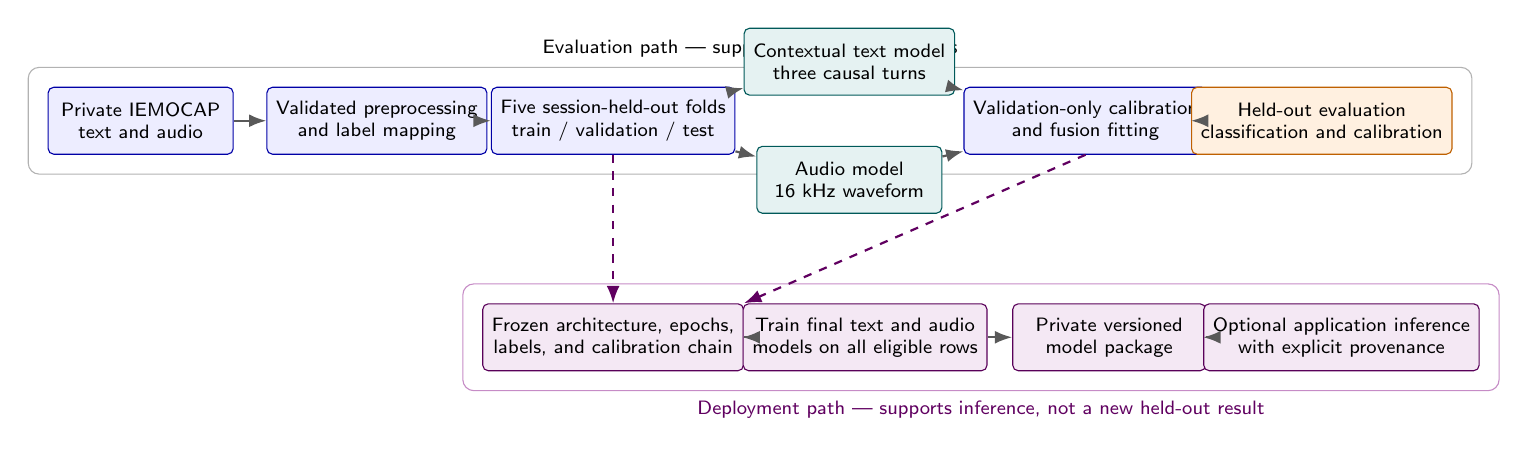
\begin{tikzpicture}[
    font=\sffamily\scriptsize,
    pipelineStep/.style={draw=blue!65!black, fill=blue!7, rounded corners=2pt,
        align=center, minimum width=2.35cm, minimum height=0.85cm},
    model/.style={draw=teal!70!black, fill=teal!10, rounded corners=2pt,
        align=center, minimum width=2.35cm, minimum height=0.85cm},
    result/.style={draw=orange!75!black, fill=orange!12, rounded corners=2pt,
        align=center, minimum width=2.5cm, minimum height=0.85cm},
    deploy/.style={draw=violet!70!black, fill=violet!9, rounded corners=2pt,
        align=center, minimum width=2.45cm, minimum height=0.85cm},
    flow/.style={-{Latex[length=2.2mm]}, thick, draw=black!65},
    freeze/.style={-{Latex[length=2.2mm]}, thick, dashed, draw=violet!75!black}
]
\node[pipelineStep] (raw) at (0,1.5) {Private IEMOCAP\\text and audio};
\node[pipelineStep] (prep) at (3.0,1.5) {Validated preprocessing\\and label mapping};
\node[pipelineStep] (folds) at (6.0,1.5) {Five session-held-out folds\\train / validation / test};
\node[model] (text) at (9.0,2.25) {Contextual text model\\three causal turns};
\node[model] (audio) at (9.0,0.75) {Audio model\\16 kHz waveform};
\node[pipelineStep] (cal) at (12.0,1.5) {Validation-only calibration\\and fusion fitting};
\node[result] (eval) at (15.0,1.5) {Held-out evaluation\\classification and calibration};

\draw[flow] (raw) -- (prep);
\draw[flow] (prep) -- (folds);
\draw[flow] (folds) -- (text);
\draw[flow] (folds) -- (audio);
\draw[flow] (text) -- (cal);
\draw[flow] (audio) -- (cal);
\draw[flow] (cal) -- (eval);

\node[deploy] (frozen) at (6.0,-1.25) {Frozen architecture, epochs,\\labels, and calibration chain};
\node[deploy] (full) at (9.2,-1.25) {Train final text and audio\\models on all eligible rows};
\node[deploy] (package) at (12.3,-1.25) {Private versioned\\model package};
\node[deploy] (inference) at (15.25,-1.25) {Optional application inference\\with explicit provenance};

\draw[freeze] (folds.south) -- (frozen.north);
\draw[freeze] (cal.south) -- (frozen.north east);
\draw[flow] (frozen) -- (full);
\draw[flow] (full) -- (package);
\draw[flow] (package) -- (inference);

\begin{scope}[on background layer]
  \node[fit=(raw)(eval), draw=black!30, rounded corners=4pt, inner sep=7pt,
      label={[font=\sffamily\scriptsize]above:Evaluation path --- supports performance claims}] {};
  \node[fit=(frozen)(inference), draw=violet!45, rounded corners=4pt, inner sep=7pt,
      label={[font=\sffamily\scriptsize, text=violet!75!black]below:Deployment path --- supports inference, not a new held-out result}] {};
\end{scope}
\end{tikzpicture}
}
\caption{Emotion-recognition evaluation and deployment pipeline. The lower path packages a frozen configuration for inference but does not create a new held-out performance result.}
\label{fig:emotion-pipeline}
\end{figure}

\subsection{Dataset Preparation and Label Mapping}
\label{subsec:dataset-preparation-label-mapping}

IEMOCAP contains dyadic scripted and improvised sessions with aligned transcripts, sentence-level audio, categorical annotations, and dimensional ratings \,\cite{busso2008iemocap}. Access to the release is restricted, so the preprocessing code operates on a privately obtained archive and does not place raw media or row-level derived data in the repository. The text preparation command can extract only annotation and transcription files from the archive. It rejects absolute paths and parent-directory traversal before extraction, and the audio preparation command applies equivalent path validation when creating the private task-specific audio bundle.

Annotation and transcript lines are joined by the IEMOCAP utterance identifier. For every usable row, preprocessing records the session, speaker, dialogue, timing, original categorical label, valence, arousal, dominance, transcript, and the expected location of the corresponding sentence-level waveform. Duplicate categorical annotations and missing transcripts cause preprocessing to stop. The resulting manifest records the source archive metadata, source-label counts, task definitions, split composition, per-class counts, and a SHA-256 digest of the manifest contents.

Table~\ref{tab:iemocap-label-mapping} shows the implemented label mappings. The deployed pipeline uses the conventional four-class task: happiness and excitement are merged, while anger, neutrality, and sadness remain separate. This produces 5,531 unique paired utterances. The code also retains an exploratory six-class task aligned more closely with the application vocabulary. That task preserves frustration, maps IEMOCAP fear to the operational label \emph{anxiety}, and renames the merged happiness/excitement class as \emph{joy}. It is not used by the deployed multimodal service, in part because the source corpus contains too few fear examples to support a stable application-facing anxiety model.

\begin{table}[htbp]
\centering
\caption{IEMOCAP source-label mappings implemented for the two experimental tasks.}
\label{tab:iemocap-label-mapping}
\footnotesize
\begingroup
\setlength{\tabcolsep}{5pt}
\begin{tabular}{|l|l|l|}
\hline
\textbf{IEMOCAP label} & \textbf{Four-class benchmark} & \textbf{Exploratory six-class task} \\ \hline
\texttt{ang} (anger) & anger & anger \\ \hline
\texttt{hap} (happiness) & happiness & joy \\ \hline
\texttt{exc} (excitement) & happiness & joy \\ \hline
\texttt{neu} (neutral) & neutral & neutral \\ \hline
\texttt{sad} (sadness) & sadness & sadness \\ \hline
\texttt{fea} (fear) & excluded & anxiety \\ \hline
\texttt{fru} (frustration) & excluded & frustration \\ \hline
\end{tabular}
\endgroup
\end{table}

The fold construction uses complete recording sessions rather than randomly partitioning utterances. For test session $s \in \{1,\ldots,5\}$, the preceding session is used for validation, with Session~5 preceding Session~1 cyclically, and the remaining three sessions form the training split. Because each of the ten actors belongs to exactly one IEMOCAP session, this arrangement keeps speakers disjoint across training, validation, and test data. Preprocessing explicitly computes the speaker sets and aborts if any overlap is detected. Across the five folds, each session appears once as held-out test data.

The private audio bundle contains exactly the sentence-level waveforms referenced by the four-class rows and names them only by utterance identifier. During creation, every expected file must be found. The script audits sample rates, channel counts, sample widths, durations, byte totals, source-archive identity, and the final bundle hash. The recorded corpus audit confirms that all 5,531 packaged files are mono 16~kHz, 16-bit PCM. Raw and processed data remain outside Git and the OneDrive-backed repository, and the bundle manifest is retained beside the private archive for integrity checking.

\subsection{Contextual Text-Emotion Model}
\label{subsec:contextual-text-emotion-model}

The textual classifier uses \texttt{microsoft/deberta-v3-small}, a compact DeBERTaV3 encoder whose pre-training combines disentangled representations with replaced-token detection and gradient-disentangled embedding sharing \,\cite{he2021debertav3}. A classification head maps the encoded input to logits in the fixed order anger, happiness, neutral, and sadness. The same training program also supports the exploratory six-class label order through configuration rather than a separate model implementation.

Two input formats are implemented. The utterance-only baseline receives the target transcript with a maximum token length of 128. The contextual model receives at most the preceding three turns from the same dialogue followed by the target utterance, with a maximum length of 256 tokens. Previous turns are ordered by their annotated start time and are marked relative to the target speaker:

\begin{equation}
x_i = [r_{i-k}]\,u_{i-k} \; \Vert \; \cdots \; \Vert \; [r_{i-1}]\,u_{i-1} \; \Vert \; [\mathrm{target}]\,u_i,
\label{eq:implementation-context-input}
\end{equation}

where $k=\min(3,i-1)$, $u_i$ is the target utterance, $r_j$ is either \texttt{same speaker} or \texttt{other speaker}, and $\Vert$ denotes concatenation with a line separator. Future turns, affect labels, dimensional annotations, and dialogue outcomes are never included. The backend reproduces this format from the last three available session turns so that training and deployment use the same causal information boundary.

For each fold, the encoder and classification head are fine-tuned with seed 42. The primary configuration uses a learning rate of $2\times10^{-5}$, weight decay of 0.01, a 10\% warm-up period, training batches of 16, evaluation batches of 32, and at most eight epochs. Validation occurs after each epoch, the checkpoint with the highest validation macro F1 is restored, and training stops after two consecutive epochs without improvement. Trainable weights begin in 32-bit floating point; mixed 16-bit computation is enabled when a compatible graphics processor is available. The four-class task uses ordinary cross-entropy, whereas the optional six-class configuration supports inverse-frequency weights clipped to a declared maximum of 10 to constrain the effect of rare categories.

Each run stores the selected model and tokenizer together with its task, label order, seed, split sessions, class weights, training history, software environment, validation and test metrics, calibrated probabilities, per-class measurements, row-level prediction files, and confusion matrix. The utterance-only and contextual experiments use the same fold membership and identifiers, permitting paired comparison by complete dialogue rather than treating correlated turns as independent samples. Quantitative comparisons between these configurations are reported in Chapter~\ref{chap5}.

After the fold experiments were frozen, the final contextual text artefact was trained for seven epochs on all 5,531 unique benchmark rows. The epoch count was derived from the completed cross-validation training behaviour rather than selected from the final full-data loss. Before training, the packaging code reconstructs the complete dataset from one fold, rejects duplicate identifiers, and requires the expected row count. The resulting artefact is intended only for inference; its training metrics do not replace the speaker-independent fold evaluation.

\subsection{Speech-Emotion Model}
\label{subsec:speech-emotion-model}

The acoustic classifier fine-tunes \texttt{facebook/wav2vec2-base}, which learns speech representations from raw waveform input through self-supervised pre-training \,\cite{baevski2020wav2vec}. The same four-class output order is used as for text so that probability vectors can be paired without remapping. Training and inference load audio from memory or private local storage; the application database never provides audio as model-training data.

Waveforms are read as 32-bit floating-point samples. A multi-channel recording, if encountered, is averaged to mono. Audio with a different sampling rate is converted to 16~kHz by polyphase resampling, and only the first 20 seconds are supplied to the model. Shorter examples are padded dynamically within each batch by the model's feature extractor. Before a fold begins, an audio audit verifies that every metadata row has a matching waveform and records the observed sample rates, maximum duration, and number of examples requiring truncation.

The convolutional feature encoder is frozen during fine-tuning, while the transformer and classification layers remain trainable. The configured learning rate is $1\times10^{-5}$ with weight decay 0.01, 10\% warm-up, a per-device batch size of four, and four gradient-accumulation steps, producing an effective batch of 16 before distributed effects. Gradient checkpointing reduces memory use. Training runs for at most ten epochs, evaluates once per epoch, restores the checkpoint with the highest validation macro F1, and applies the same two-epoch early-stopping patience as the text experiment. GPU execution uses mixed precision when available.

Audio runs write the trained feature extractor and classifier along with the fold, label order, seed, split sessions, audio audit, environment versions, training history, validation-calibration parameters, test distributions, per-class measurements, and confusion matrix. Validation and test identifiers must match those of the contextual text run before fusion can proceed. Following the fold experiments, the deployable audio artefact is trained for ten epochs on the same 5,531 unique examples used by the final text model. As with the final text artefact, this is a packaging run rather than a new evaluation.

\subsection{Multimodal Late Fusion}
\label{subsec:multimodal-late-fusion}

Text and speech are combined through decision-level late fusion rather than by joining their hidden representations. This choice keeps each modality independently trainable, inspectable, and usable in ablation analysis, and it avoids retraining a joint network when the fusion policy changes \,\cite{baltrusaitis2019multimodal}. Before any distributions are combined, the fusion program verifies the label order, exact utterance-identifier set, expected label, recorded fold number, and reconstruction of the saved single-modality metrics. It also rejects an utterance that appears in the test output of more than one fold.

Let $z_t$ and $z_a$ denote text and audio logits, and let $T_t$ and $T_a$ be their validation-fitted temperatures. The calibrated modality distributions are

\begin{equation}
p_t = \operatorname{softmax}\!\left(\frac{z_t}{T_t}\right), \qquad
p_a = \operatorname{softmax}\!\left(\frac{z_a}{T_a}\right).
\label{eq:implementation-modality-calibration}
\end{equation}

Given text weight $w$, the intermediate fusion is a convex combination,

\begin{equation}
p_m = w p_t + (1-w)p_a.
\label{eq:implementation-late-fusion}
\end{equation}

The research comparison uses a predeclared equal-weight setting, $w=0.5$, so that the hypothesis that audio contributes complementary information is not assessed using a weight selected from the held-out test predictions. A separate deployment-calibration path fits $w$ over the fixed grid $\{0.00,0.01,\ldots,1.00\}$ using paired validation predictions and validation negative log-likelihood only. After choosing the weight, it fits a final scalar temperature $T_f$ and calculates

\begin{equation}
p_f = \operatorname{softmax}\!\left(\frac{\log(\max(p_m,10^{-12}))}{T_f}\right).
\label{eq:implementation-fusion-calibration}
\end{equation}

For the packaged full-data models, the deployable parameters were fitted from 5,531 pooled validation-role predictions. Pooling changes the evidential status of the subsequent summary: across the five rotating folds, every utterance identity and label contributes once to this global fit and also once to the pooled test-role predictions used to describe the fitted chain, although the two predictions come from different trained models. The resulting metrics are therefore not an independent held-out evaluation. They are retained only as an operational packaging analysis for choosing one parameter set for the full-data models. The frozen configuration contains $T_t=1.8268$, $T_a=1.3357$, $w=0.59$ for text, $1-w=0.41$ for audio, and $T_f=0.5989$; these values are applied unchanged by the backend. Confirmatory performance claims instead use the predeclared equal-weight comparison and the fold-specific configuration in which each test session's labels did not participate in fitting that fold's parameters.

\subsection{Confidence Calibration and Uncertainty Handling}
\label{subsec:confidence-calibration-uncertainty}

For each single-modality fold, temperature scaling fits one positive scalar on validation logits by minimising negative log-likelihood \,\cite{guo2017calibration}. The implementation searches in log-temperature space and never uses the test session during fitting. Dividing every class logit by the same temperature changes the probability concentration without changing the class with maximum logit. Calibration is consequently evaluated separately from classification performance.

The evaluation utilities compute accuracy, macro F1, weighted F1, per-class precision, recall and F1, negative log-likelihood, multiclass Brier score, and expected calibration error. Expected calibration error partitions maximum confidence into fixed bins and accumulates the sample-weighted difference between mean confidence and empirical accuracy. Row-level outputs retain the complete probability vector rather than only the winning label, enabling later reliability analysis and exact pairing between modalities. Statistical comparisons use paired percentile bootstrap samples at dialogue level so that multiple turns from one conversation remain in the same resampled unit; those results belong to the evaluation chapter rather than the implementation account.

At inference time, the backend returns the calibrated text, audio, and fused distributions, each modality's selected label and confidence, and an explicit indicator of whether the two modalities agree. Fused confidence below 0.55 is labelled \emph{low}, confidence from 0.55 up to 0.75 is labelled \emph{moderate}, and confidence at or above 0.75 is labelled \emph{high}. The adaptation policy uses the configurable 0.55 low-confidence boundary for the fused, textual, and acoustic confidences; the 0.75 boundary names the high presentation band but does not impose a further adaptation gate. These boundaries do not modify the model probabilities, turn a prediction into a verified emotion, or establish that estimates above them are correct.

Missing, invalid, conflicting, or low-confidence evidence is represented explicitly rather than converted into a stronger claim. The role-play workflow remains usable without audio or trained inference, and the dialogue policy and crisis checks do not depend on the predicted category. Calibration measured on IEMOCAP may deteriorate under changes in speakers, microphones, language, interaction style, or context \,\cite{ovadia2019shift}. The application therefore treats confidence and cross-modal agreement as bounded operational signals, not as guarantees of correctness.

\subsection{Model Artefacts, Provenance, and Inference Loading}
\label{subsec:model-artefacts-provenance}

The final private package contains one contextual-text model directory and one audio-model directory. Each directory includes the saved classifier and the associated tokenizer or feature extractor. The versioned multimodal JSON configuration stores the label order, input field, maximum text length, sample rate, waveform-duration limit, model names, optimisation settings, and complete calibration chain. Model weights and licensed data are excluded from Git; a synchronisation script retrieves the final directories from private cloud storage into a user-selected local destination and prints the corresponding environment settings.

Provenance is captured after the private models are downloaded. The provenance command records the current source-control commit, SHA-256 of the multimodal configuration, Python platform, relevant library versions, and, for every file in both model directories, its relative path, size, and SHA-256 digest. It also calculates an aggregate directory digest from the ordered file entries. This manifest binds an inference result to specific model contents and code configuration without publishing the restricted artefacts themselves.

The backend keeps multimodal inference disabled by default. When enabled, it checks that both model directories and the configuration exist, then loads the tokenizer, feature extractor, and classifiers lazily on the first request. Device selection uses an available CUDA device when configured as automatic and otherwise uses the requested device or CPU. Models are placed in evaluation mode and executed under the framework's inference-only context. A process-level asynchronous lock serialises multimodal requests so that simultaneous users do not compete unpredictably for model memory; model execution is moved to a worker thread so that the asynchronous web loop remains responsive. Queue and inference times are returned separately.

Before inference, the service checks the configured byte limit, parses the in-memory WAV payload, requires a duration between 0.25 and 35 seconds, converts multi-channel audio to mono, resamples when required, and truncates model input to the configured 20-second maximum. Text context is constructed from the latest three causal turns using the same speaker-relative markers as training. The service then applies the stored modality temperatures, weighted fusion, and fusion temperature exactly as defined in Equations~\ref{eq:implementation-modality-calibration}--\ref{eq:implementation-fusion-calibration}. Its response includes the distributions, agreement, confidence level, model version, latency, queue time, and an explicit statement that audio was not persisted.

Two forms of validation protect the packaged artefacts. Unit tests check causal context construction, confidence boundaries, disabled-service behaviour, and serialisation of concurrent requests without importing machine-learning libraries when inference is disabled. A private integrity smoke test selects an equal number of examples from each class, loads both final models, verifies finite logits and probabilities, runs the frozen fusion chain, and requires each component to predict more than one class. Any accuracy calculated on this balanced training sample is labelled as an integrity diagnostic and is not reported as evaluation performance. If loading or inference fails in the application, the failure remains contained within the optional service and the text-first rehearsal workflow continues through its deterministic path.
%
\section{Backend Application}
\label{sec:backend-application}

The backend application is the authoritative coordination layer between the browser, persistence store, dialogue policies, safety checks, trained models, and optional external providers. It exposes a JSON API below the \texttt{/api} prefix, but keeps transport concerns separate from the rules that govern a rehearsal. Consequently, neither the frontend nor a language-model response can directly alter dialogue state, feedback evidence, study status, or resource ownership. These changes are performed by typed backend services and persisted through a repository interface.

This section describes the general backend infrastructure and the lifecycle of a conversation request. The implementation of the role-play policy, feedback calculations, research workflow, and detailed security controls is developed in the subsequent sections.

\subsection{Application and Service Architecture}
\label{subsec:backend-service-architecture}

The FastAPI application is assembled from four principal layers. API routes form the HTTP boundary and translate expected service failures into suitable status codes. Pydantic schemas validate transport data and constrain the response shape. Application services implement authentication, conversation coordination, transcription, multimodal analysis, preparation, branching, and research operations. Finally, repositories encapsulate all mutable storage. The domain models are shared between the service and repository layers, while external-provider clients remain behind dedicated service classes. This arrangement prevents route functions from becoming an alternative location for dialogue or persistence logic.

Service construction is centralised in a small application container. At process start, configuration selects either the MongoDB repository or its in-memory substitute, after which one authentication service, conversation service, multimodal service, transcription service, and email service is constructed. FastAPI dependencies provide these instances and the authenticated user to individual routes. The conversation service itself depends on interfaces for emotion analysis, cognitive analysis, strategy selection, response generation, and persistence. Default deterministic implementations can therefore be replaced without changing the route contract or the stored session representation.

The application lifespan initialises repository indexes before accepting normal work. In offline demonstration mode it also creates the local demonstration account if required; this mode is rejected by production configuration. Existing eligible sessions are then used to backfill any missing study records. A separate liveness endpoint confirms that the process is running, whereas the readiness endpoint validates configuration, checks the persistence connection and required indexes, and reports the availability of optional transcription and multimodal services. A missing optional model does not make the text-first application unready.

Cross-cutting HTTP behaviour is installed as middleware. Configured origins control credentialled cross-origin requests, trusted-host validation rejects unexpected host headers, and production deployments redirect HTTP traffic to HTTPS. Response middleware adds restrictive framing, content-type, referrer, permissions, caching, and content-security headers, together with HTTP Strict Transport Security in production. A configurable rate limiter applies separate windows to authentication, email, transcription, and model-backed operations. It is intentionally a single-instance implementation; a horizontally scaled deployment would require a shared limiter at a gateway or distributed store.

\subsection{Domain Models and API Schemas}
\label{subsec:backend-domain-models}

The domain layer represents application state as nested Pydantic models rather than unstructured dictionaries. Its enumerations constrain concepts such as speaker role, difficulty, practice goal, role-play status, support strategy, and user intent. A \texttt{Session} owns its ordered turns, current emotion state, optional role-play state, feedback, action card, questionnaires, research events, version, and expiry time. Each \texttt{ConversationTurn} may retain the emotion state observed at that point, selected strategy, response-generation metadata, and the bounded affect-pacing decision. More detailed role-play models preserve dialogue snapshots, evidence linked to source turns, reason codes, policy versions, branch lineage, and feedback comparisons. This makes the recorded session an auditable account of state transitions rather than only a transcript.

Transport schemas are deliberately distinct from these persistent entities. Request models impose limits before data reaches a service: messages are non-empty and limited to 5,000 characters, session titles to 80 characters, takeaways to 500 characters, and encoded audio to 7,000,000 characters. Enumerated fields constrain pacing preferences and difficulty settings, strict Boolean fields prevent ambiguous coercion for decisions such as eligibility confirmation, and selected request objects reject unknown properties. Responses expose only the fields needed by the relevant interface; for example, the public user response omits the password hash and token records held by the domain and repository layers.

Validation also protects relationships between fields. An enhanced chat exchange that requests audio analysis, affect adaptation, or non-default pacing must supply both a unique request identifier and the version of the session displayed by the client. Questionnaire schemas restrict ratings to their declared scales, and service validation checks that all required answers are submitted together or explicitly skipped. A multimodal estimate is accepted only when every probability is finite and within the unit interval, each distribution sums to approximately one, and the declared label and confidence agree with its maximum entry. Agreement and confidence-band fields are then derived again on the backend instead of being trusted from an external payload.

The domain models also distinguish operational metadata from user-facing content. Generated responses record their source, model, latency, token counts, and any fallback reason. Affect decisions record availability, user preference, inference timing, confidence, and the selected pacing action. Study records contain pseudonymous participant and protocol identifiers rather than copying the complete account. These explicit fields allow later analysis to separate deterministic and provider-backed behaviour, while preventing absent measurements from being interpreted as observed zero values.

\subsection{Authentication and Account Management}
\label{subsec:backend-authentication}

Registration requires acceptance of the current privacy terms. Email addresses are normalised before storage and a unique database index prevents duplicate accounts. Passwords are processed by the password library's recommended one-way hashing scheme; plaintext passwords are never stored. A cryptographically random verification value is sent by email, while only its SHA-256 digest and expiry time are retained. Normal login and protected routes require a verified email address. Registration, verification resend, and password-recovery endpoints return deliberately generic messages so that their responses do not reveal whether a supplied address belongs to an account.

Successful authentication issues two tokens with different handling. The short-lived JSON Web Token used for API authorisation is returned to the browser and presented as a bearer credential. The longer-lived refresh token is placed in an HTTP-only, same-site cookie scoped to the authentication routes and marked secure in production. Its identifier and digest are stored server-side. Refreshing atomically removes the presented record and creates a replacement, so a token cannot be successfully rotated twice. Logout, password change, password reset, and account deletion revoke the user's outstanding refresh tokens; password-reset links are likewise digest-only, expiring, and consumed atomically after the replacement password has passed validation.

The dependency that resolves the current user decodes the access token, reloads the account, and checks email verification on every protected request. This means deletion or loss of eligibility is observed by later calls rather than being determined solely by claims in an old access token. Researcher routes add a second dependency that compares the verified account email with the configured researcher allow-list. Participant study enrolment is a separate state transition and does not implicitly grant researcher privileges.

Profile and lifecycle operations are handled through the same authenticated service boundary. Users can update the constrained profile fields, choose between one and three distinct practice goals during onboarding, change their password, sign out, or delete their account. Account deletion cascades through sessions, study records, refresh tokens, and outstanding verification and recovery records in both repository implementations. Study withdrawal has a narrower, protocol-specific meaning and is therefore implemented independently from deletion; the later research-workflow section describes this distinction in detail.

\subsection{Session Persistence and Ownership Controls}
\label{subsec:backend-session-persistence}

The repository contract supplies identical account, session, token, study-record, lifecycle, and frozen-export operations for the in-memory and MongoDB implementations. The in-memory implementation supports isolated development and fast unit tests; the MongoDB implementation supplies durable storage for the integrated application. Services depend only on this contract, so choosing a persistence backend does not introduce database-specific branches into conversation processing.

Session ownership is enforced as part of repository queries. Reading or deleting a session requires both its identifier and the authenticated user's identifier, and session listings are filtered by the same user key. Expired sessions are excluded from reads, while a MongoDB time-to-live index removes them according to their \texttt{expires\_at} value. Thus, knowing another session's universally unique identifier is insufficient to retrieve or mutate it. Service methods translate a failed owned lookup into the same not-found result, avoiding a distinction between a missing resource and one owned by somebody else.

Every session also carries a monotonically increasing version. When the enhanced chat interface submits an exchange, it includes the displayed version and a request identifier. The conversation service rejects a repeated request identifier or stale version before modifying a deep copy of the session. At the storage boundary, MongoDB replaces a document only when its stored version equals the service's expected version, then increments it; an insert collision or failed conditional replacement becomes a concurrent-update error. The in-memory repository implements the same comparison. The global exception handler returns HTTP status 409 with instructions to reload, preventing two tabs or overlapping requests from silently overwriting one another.

MongoDB indexes additionally enforce unique email, session, study-record, protocol, and frozen-export identifiers, support per-user chronological queries, and expire session, token, and study records at their respective deadlines. Readiness checks verify these indexes rather than assuming they were created. Conversation and consented research data remain separate: a session contains the complete interaction needed by the application, whereas the synchronised study record contains protocol-bounded events, measures, generation counts, and feedback metrics under its own retention rule. The later research-workflow and data-protection sections describe the detailed minimisation and withdrawal behaviour.

\subsection{Conversation Request Processing}
\label{subsec:backend-conversation-processing}

The \texttt{/api/chat} endpoint is intentionally a thin coordinator. After schema validation and authentication, it delegates the message, account identity, optional audio, affect preference, request identifier, and expected session version to the conversation service. The service first performs the owned session lookup and the duplicate and stale-version checks described above. If necessary, the first message supplies a shortened default title; beginning a new exchange also closes an unused immediate post-questionnaire opportunity so that questionnaire timing cannot drift into later conversation.

Safety evaluation precedes affect adaptation and response generation. A local crisis-language check always runs, and provider moderation may add a flag when the provider is configured. If a crisis is detected, optional multimodal inference is skipped, the fixed safety response takes precedence, and an active or paused rehearsal is marked as interrupted. The trained affect model is therefore neither a prerequisite nor an authority for crisis handling.

For a non-crisis exchange, multimodal inference is attempted only when the request is bound to a version and request identifier, audio is present, a configured model is available, and the rehearsal is eligible for experimental adaptation. It is deliberately excluded from required study tasks so that the required protocol path is not altered by this optional condition. Decoding, validation, or inference failure is caught and recorded as unavailable rather than aborting the message. Independently, the local text analyser updates the smoothed emotion state, the cognitive analyser derives tentative intent and readiness features, and the scored selector chooses a support strategy with its component scores and reason codes.

The user turn is appended before reply selection. During an active rehearsal, the deterministic role-play engine advances the dialogue state, links observed evidence to that turn, and supplies both a required character action and safe fallback wording. Outside role-play, the selected support strategy guides the general response generator. An affect-pacing prefix may be added only through the bounded pacing policy and only under its eligibility conditions. The resulting assistant turn stores generation and affect-decision metadata; role-play decisions additionally store before-and-after snapshots, evidence identifiers, policy versions, and reason codes.

Finally, the service records a minimised completion event, updates measurement boundaries when a rehearsal ends, persists the incremented session, and synchronises an eligible study record. The response returns the committed version together with the user and assistant turns, decision summary, current role-play state, any completed feedback, and the one-use opportunity token required for an immediate post-rehearsal questionnaire. This single service path keeps the dialogue shown by the client aligned with the state and evidence retained by the backend.

The ordering and alternative paths are summarised in Figure~\ref{fig:request-sequence}. In particular, the safety branch terminates ordinary processing before optional affect inference and response generation.

\begin{figure}[p]
\centering
\resizebox{\textwidth}{!}{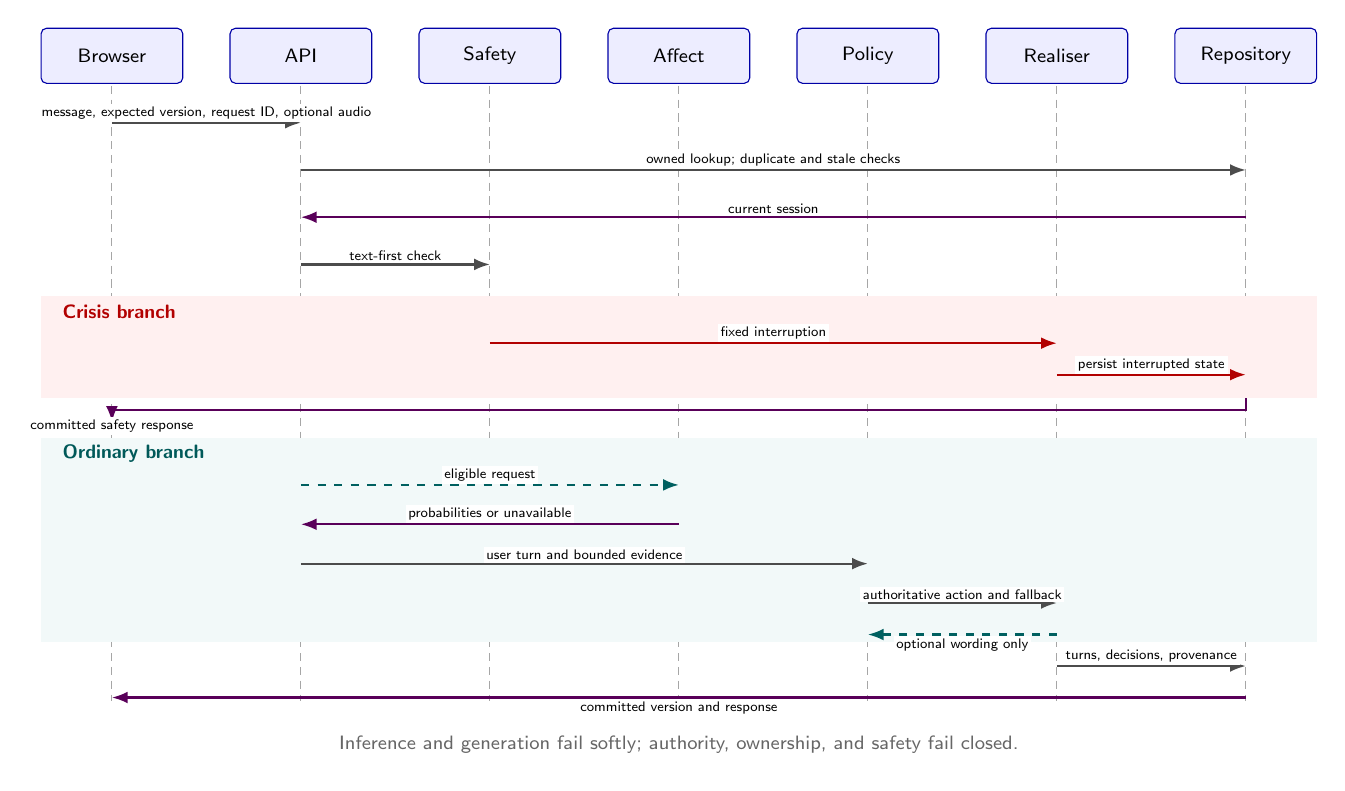
\begin{tikzpicture}[
    font=\sffamily\scriptsize,
    actor/.style={draw=blue!65!black, fill=blue!7, rounded corners=2pt,
        align=center, minimum width=1.8cm, minimum height=0.7cm},
    msg/.style={-{Latex[length=2mm]}, draw=black!70, thick},
    optional/.style={-{Latex[length=2mm]}, draw=teal!75!black, dashed, thick},
    return/.style={-{Latex[length=2mm]}, draw=violet!70!black, thick},
    note/.style={font=\sffamily\tiny, fill=white, inner sep=1pt}
]
\foreach \name/\label/\x in {
 ui/Browser/0,
 api/API/2.4,
 safety/Safety/4.8,
 affect/Affect/7.2,
 policy/Policy/9.6,
 realise/Realiser/12.0,
 repo/Repository/14.4}
{
  \node[actor] (\name) at (\x,0) {\label};
  \draw[densely dashed, black!35] (\x,-0.38) -- (\x,-8.2);
}

\draw[msg] (0,-0.85) -- node[note, above]{message, expected version, request ID, optional audio} (2.4,-0.85);
\draw[msg] (2.4,-1.45) -- node[note, above]{owned lookup; duplicate and stale checks} (14.4,-1.45);
\draw[return] (14.4,-2.05) -- node[note, above]{current session} (2.4,-2.05);
\draw[msg] (2.4,-2.65) -- node[note, above]{text-first check} (4.8,-2.65);

\fill[red!6] (-0.9,-3.05) rectangle (15.3,-4.35);
\node[anchor=west, text=red!70!black, font=\sffamily\bfseries\scriptsize]
    at (-0.75,-3.25) {Crisis branch};
\draw[msg, draw=red!70!black] (4.8,-3.65) -- node[note, above]{fixed interruption} (12.0,-3.65);
\draw[msg, draw=red!70!black] (12.0,-4.05) -- node[note, above]{persist interrupted state} (14.4,-4.05);
\draw[return] (14.4,-4.35) -- ++(0,-0.15) -| node[pos=0.75, note, below]{committed safety response} (0,-4.65);

\fill[teal!5] (-0.9,-4.85) rectangle (15.3,-7.45);
\node[anchor=west, text=teal!70!black, font=\sffamily\bfseries\scriptsize]
    at (-0.75,-5.05) {Ordinary branch};
\draw[optional] (2.4,-5.45) -- node[note, above]{eligible request} (7.2,-5.45);
\draw[return] (7.2,-5.95) -- node[note, above]{probabilities or unavailable} (2.4,-5.95);
\draw[msg] (2.4,-6.45) -- node[note, above]{user turn and bounded evidence} (9.6,-6.45);
\draw[msg] (9.6,-6.95) -- node[note, above]{authoritative action and fallback} (12.0,-6.95);
\draw[optional] (12.0,-7.35) -- ++(-2.4,0) node[midway, note, below]{optional wording only};
\draw[msg] (12.0,-7.75) -- node[note, above]{turns, decisions, provenance} (14.4,-7.75);
\draw[return] (14.4,-8.15) -- node[note, below]{committed version and response} (0,-8.15);

\node[align=center, text=black!60] at (7.2,-8.75)
    {Inference and generation fail softly; authority, ownership, and safety fail closed.};
\end{tikzpicture}
}
\caption{Sequence of a version-bound conversation request, including safety precedence and failure-tolerant optional processing.}
\label{fig:request-sequence}
\end{figure}

\subsection{Optional Services and Deterministic Fallbacks}
\label{subsec:backend-fallbacks}

Network-dependent and model-dependent functions are implemented as enhancements rather than foundations of the rehearsal workflow. When an OpenAI API key is present, the response generator can realise a selected support strategy in natural language, moderate text, phrase evidence-based feedback, or render a role-play action. Requests use a configured timeout and disable provider-side response storage. If credentials are absent, the service is disabled, a call raises an exception, or a response is empty, refused, or structurally invalid, generation returns the corresponding deterministic template and records the fallback reason.

Provider output is constrained differently according to its purpose. General support generation receives the authoritative emotion state and selected strategy together with instructions against diagnosis, medication advice, certainty claims, and dependency. Role-play realisation receives the authoritative scenario, difficulty behaviour, state, and required action, and must return a typed action and a short in-character utterance. Outputs that expose coaching language or disagree with the required action are discarded. Where the enhanced dialogue policy contains a concrete negotiated constraint or proposal, exact deterministic wording remains in force until semantic validation can reliably establish that a rephrasing preserves it. Feedback generation is limited to rewording strengths and suggestions that have already been calculated from recorded evidence; it cannot create new observations or scores.

Transcription and trained multimodal inference use separate authenticated endpoints and report explicit unavailability when invoked directly without configuration. In the integrated chat path, multimodal failure is contained and the deterministic exchange continues. Audio is size-checked and decoded in memory for the immediate operation, and service responses state that it was not persisted. Email delivery is similarly isolated behind its service boundary; generic account responses remain stable when delivery fails, without falsely granting verification or recovery access.

Each generated turn records whether its content came from a template, safety response, deterministic role-play path, or configured provider, together with latency and fallback information where available. Health and model-information endpoints expose capability status without treating an optional dependency as a core outage. These choices preserve an operational baseline in offline demonstrations, tests, and provider failures, while making the provenance of enhanced behaviour visible for debugging and later evaluation.
%
\subsection{Rule-Based Cognitive Features and Support Routing}
\label{subsec:cognitive-support-routing}

The class named \texttt{RuleBasedCognitiveAnalyzer} is a deterministic phrase matcher applied to the current text; ``cognitive'' is an implementation name rather than a claim that the component performs cognitive or clinical assessment. It checks ten authored regular-expression families labelled mind-reading, catastrophising, overgeneralisation, all-or-nothing thinking, should statements, emotional reasoning, fortune-telling, personalisation, discounting positives, and labelling. A matching family receives a fixed rule weight and the highest-weight family is returned as a ``possible'' pattern. The number is neither a learned probability nor a severity score. The rules have no access to clinical history, speaker identity, longitudinal belief patterns, or professional annotations.

The remaining fields are equally mechanical. Intent follows a fixed precedence: explicit rehearsal terms, practical-help terms, emotion or validation terms, a question mark, and otherwise unclear. ``Readiness for advice'' is assigned one of four constants according to those same matches; it is not estimated from observed acceptance of advice. ``Resistance'' is 0.7 for four explicit pushback phrases, 0.15 for any other occurrence of ``but'', and zero otherwise. ``Possible cause'' copies up to 100 characters following \emph{because}, \emph{after}, \emph{when}, or \emph{since}. Boolean request flags repeat the rehearsal, practical-help, and validation matches. These definitions make the output reproducible but also expose obvious failure modes involving negation, quotation, sarcasm, polysemy, indirect requests, multiple clauses, and dialectal or multilingual wording.

Outside active role-play, \texttt{ScoredStrategySelector} converts the heuristic record and lexical affect state into additive priorities for validation, reflection, clarification, validate--reframe, practical suggestion, rehearsal invitation, de-escalation, and safety escalation. For example, an explicit rehearsal phrase favours an invitation to practise; a practical-help match with its associated fixed readiness value favours a suggestion; a cognitive-pattern match favours validate--reframe; and one of the four strong pushback phrases favours reflection while reducing the suggestion score. The maximum total selects the strategy supplied to the response generator. These strategy scores express rule priority, not the probability that a response is suitable or effective.

The subsystem has deliberately limited authority. Crisis handling is evaluated first and forces the safety strategy. During active role-play, the scenario controller selects the character action, so cognitive tags cannot advance a stage, declare success, or alter feedback scores. The subsystem does affect general supportive responses and its intent, possible pattern, possible context, selected strategy, and reasons can be displayed in the ``Why this response?'' panel. That visibility is why the feature is documented here even though it is secondary to the dissertation's emotion-recognition and rehearsal contributions. Its evidence base is limited to rule and integration tests reported in Section~\ref{subsec:cognitive-routing-results}; no corpus-level predictive validity, clinical validity, or outcome benefit has been established.

\section{Role-Play and Adaptation Engine}
\label{sec:roleplay-adaptation}

The role-play engine implements the central distinction established in the system architecture: deterministic code selects the permitted conversational action, while a generator may only realise that action in words. It therefore treats scenario progress, evidence, completion, safety, and feedback as application state rather than delegating them to a language model. The same state can be serialised, restored, replayed, rewound, and tested without a network connection.

\subsection{Scenario Representation and Configuration}
\label{subsec:scenario-representation}

A role-play scenario is represented by an identifier, title, character, situation, user objective, opening line, expected skills, difficulty-specific behaviour, success conditions, and a maximum number of turns. The repository contains six standard scenarios: workload prioritisation, maintaining a personal boundary, expressing a relationship need, giving feedback to a colleague, negotiating a deadline, and sharing household responsibilities. The first three form the standardised study sequence; the remaining scenarios broaden ordinary practice without changing the study protocol.

Difficulty is an explicit enumeration with beginner, intermediate, and difficult levels. At initialisation these levels map to increasing challenge and decreasing cooperation values, but the selected level does not change the meaning of a recorded communication feature. For standard unprofiled practice, difficulty primarily controls how much resistance the character provides and, for the boundary scenario, how many clear refusals must be maintained. Every new attempt stores its scenario, policy, and scoring versions so that later feedback and comparisons are interpreted under the rules that produced them.

Additional practice in the workload, boundary, and relationship scenarios may also use one of three authored character profiles. The cooperative profile asks for a clear practical response, the rushed profile prioritises concise decisions and a workable time, and the sceptical profile questions the proposal and may repeat pressure. These profiles select versioned deterministic policies rather than psychological personalities. They are unavailable for required study tasks and custom scenarios, preventing an optional experimental path from modifying the frozen protocol.

Users can create account-owned custom scenarios directly or through the preparation workflow. Custom inputs are normalised and limited in length, and their target skills must come from the supported observable set: clear request, specific detail, boundary maintenance, I-statements, and non-blaming language. A prepared scenario additionally stores the difficult part identified by the user and a tentative likely objection produced by a bounded local template. The template is presented for review and editing; it is not claimed to predict another person's response.

\subsection{Dialogue State and Transition Logic}
\label{subsec:dialogue-transitions}

The role-play state stores status, current stage, turn count, difficulty, cooperation, accumulated evidence, decisions, outcome, completion reason, and timestamps. It supports active, paused, completed, and interrupted states. Pausing permits reflection without advancing the rehearsal, resuming returns to the existing controller state, and manual completion remains distinct from automatic success. The maximum of eight user turns prevents an unresolved simulation from continuing indefinitely.

The enhanced scenario policy represents each supported conversation as a small state graph. Workload practice advances from explaining the problem, through addressing constraints, to agreeing a plan. Boundary practice progresses from an initial refusal, through pressure, to respectful closure. Relationship practice moves from describing the situation and need, through acknowledging the other perspective, to selecting a practical next step. A transition occurs only when the observable evidence required at the current stage has appeared; unsupported or contradictory input leaves the controller in place and produces a targeted follow-up.

The three graphs contain scenario-specific checks. For example, the workload path requires the user to acknowledge the stated delivery constraint while proposing a supported trade-off before agreement can be confirmed. The boundary path distinguishes a maintained refusal from a reversal or conditional acceptance and varies the permitted pressure rounds by difficulty and profile. The relationship path requires a specific personal need, acknowledgement of perspective, and a feasible request; unsupported or explicitly unresolved endings remain recorded as such. These rules model the authored practice exercise, not the probable behaviour of a real manager, friend, or partner.

Figure~\ref{fig:dialogue-states} presents the principal state progression for the three standardised scenarios and the explicit non-success exits shared by the controllers.

\begin{figure}[htbp]
\centering
\resizebox{\textwidth}{!}{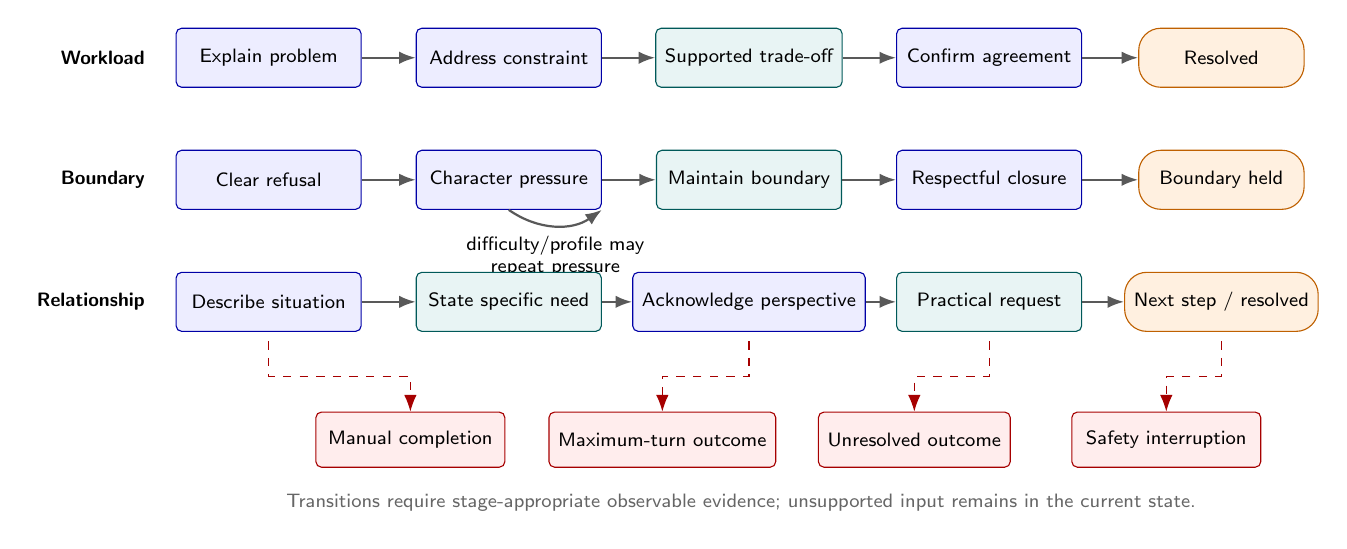
\begin{tikzpicture}[
    font=\sffamily\scriptsize,
    state/.style={draw=blue!65!black, fill=blue!7, rounded corners=2pt,
        align=center, minimum width=2.35cm, minimum height=0.75cm},
    evidence/.style={draw=teal!70!black, fill=teal!9, rounded corners=2pt,
        align=center, minimum width=2.35cm, minimum height=0.75cm},
    terminal/.style={draw=orange!75!black, fill=orange!12, rounded corners=8pt,
        align=center, minimum width=2.1cm, minimum height=0.75cm},
    exit/.style={draw=red!65!black, fill=red!7, rounded corners=2pt,
        align=center, minimum width=2.4cm, minimum height=0.7cm},
    flow/.style={-{Latex[length=2.1mm]}, thick, draw=black!65},
    stop/.style={-{Latex[length=2.1mm]}, dashed, draw=red!65!black}
]
\node[anchor=east, font=\sffamily\bfseries\scriptsize] at (-0.25,2.4) {Workload};
\node[state] (w1) at (1.2,2.4) {Explain problem};
\node[state] (w2) at (4.25,2.4) {Address constraint};
\node[evidence] (w3) at (7.3,2.4) {Supported trade-off};
\node[state] (w4) at (10.35,2.4) {Confirm agreement};
\node[terminal] (w5) at (13.3,2.4) {Resolved};
\draw[flow] (w1)--(w2); \draw[flow] (w2)--(w3); \draw[flow] (w3)--(w4); \draw[flow] (w4)--(w5);

\node[anchor=east, font=\sffamily\bfseries\scriptsize] at (-0.25,0.85) {Boundary};
\node[state] (b1) at (1.2,0.85) {Clear refusal};
\node[state] (b2) at (4.25,0.85) {Character pressure};
\node[evidence] (b3) at (7.3,0.85) {Maintain boundary};
\node[state] (b4) at (10.35,0.85) {Respectful closure};
\node[terminal] (b5) at (13.3,0.85) {Boundary held};
\draw[flow] (b1)--(b2); \draw[flow] (b2)--(b3); \draw[flow] (b3)--(b4); \draw[flow] (b4)--(b5);
\draw[flow, bend right=35] (b2.south) to node[below, align=center]{difficulty/profile may\\repeat pressure} (b2.south east);

\node[anchor=east, font=\sffamily\bfseries\scriptsize] at (-0.25,-0.7) {Relationship};
\node[state] (r1) at (1.2,-0.7) {Describe situation};
\node[evidence] (r2) at (4.25,-0.7) {State specific need};
\node[state] (r3) at (7.3,-0.7) {Acknowledge perspective};
\node[evidence] (r4) at (10.35,-0.7) {Practical request};
\node[terminal] (r5) at (13.3,-0.7) {Next step / resolved};
\draw[flow] (r1)--(r2); \draw[flow] (r2)--(r3); \draw[flow] (r3)--(r4); \draw[flow] (r4)--(r5);

\node[exit] (manual) at (3.0,-2.45) {Manual completion};
\node[exit] (limit) at (6.2,-2.45) {Maximum-turn outcome};
\node[exit] (unresolved) at (9.4,-2.45) {Unresolved outcome};
\node[exit] (safety) at (12.6,-2.45) {Safety interruption};
\draw[stop] (1.2,-1.2) -- ++(0,-0.45) -| (manual.north);
\draw[stop] (7.3,-1.2) -- ++(0,-0.45) -| (limit.north);
\draw[stop] (10.35,-1.2) -- ++(0,-0.45) -| (unresolved.north);
\draw[stop] (13.3,-1.2) -- ++(0,-0.45) -| (safety.north);

\node[align=center, text=black!60] at (7.2,-3.25)
    {Transitions require stage-appropriate observable evidence; unsupported input remains in the current state.};
\end{tikzpicture}
}
\caption{Principal dialogue-state progression for workload, boundary, and relationship rehearsal.}
\label{fig:dialogue-states}
\end{figure}

Each processed rehearsal message produces a decision record containing the before-and-after dialogue snapshots, selected character action, reason codes, linked user and assistant turns, supporting evidence identifiers, generation metadata, character profile, and scenario, policy, and scoring versions. Completion reasons distinguish success, the turn limit, manual completion, and safety interruption. Persisting these transitions makes recovery exact: a restored session does not need to infer its stage again from the transcript.

\subsection{Communication-Evidence Extraction}
\label{subsec:communication-evidence}

Evidence extraction operates on the submitted text and records bounded, inspectable language features. The common extractor identifies patterns associated with a concrete request, repeated apology, maintained boundary, blame phrasing, specific detail, and I-statements. Versioned scenario extractors add features such as a problem description, workable option, check-in, clear refusal after pressure, respectful closure, acknowledgement of perspective, and practical request. Negation, conditional language, reported speech, and contradictory clauses are handled for the specific patterns required by the authored dialogue paths.

Each evidence item records its rehearsal number and source-turn identifier. It also contains the extracted feature names and the text analyser's arousal value. It does not store an invented quotation span. The original utterance remains the authoritative source, and replay highlights the complete linked turn when exact spans were not recorded. Features may accumulate across exchanges where a scenario permits this, but completion is still controlled by stage order; mentioning an agreement before the character has raised its constraint cannot skip the intervening dialogue.

The rules intentionally favour auditability over unrestricted semantic coverage. Indirect refusals, sarcasm, unusual paraphrases, and complex multi-clause statements may be missed. A detected phrase is therefore reported as observable evidence in this rehearsal, not as proof of communication competence, intention, personality, or likely real-world success. The deterministic test fixtures include supported, negated, reversed, irrelevant, and ambiguous examples to keep this boundary visible.

\subsection{Affect-Aware Pacing Policy}
\label{subsec:affect-pacing}

The affect-pacing policy is a separate versioned layer applied after the dialogue controller has selected its response. It never changes the scenario stage, profile, difficulty, success conditions, evidence, or feedback score. Automatic use is disabled by default, and the participant may instead request that the exchange keep going unchanged, use a gentler pace, or add more challenge. An explicit choice takes precedence over automatic inference and can operate without audio.

Automatic adaptation is restricted to active, enhanced, non-required rehearsals. Required study tasks, associated retries, ordinary reflection, legacy sessions, paused or completed attempts, and ineligible scenarios use the baseline response. Safety and completed-exchange conditions take precedence. The policy also refuses to translate model categories into anxiety, readiness, resistance, or other psychological constructs; the existing lexical state tracker remains independent.

When automatic adaptation is eligible, missing audio, unavailable models, inference failure, or unsupported categories produce no addition. If any fused or component confidence is below the stored low-confidence threshold, or if the fused, text, and audio labels do not all agree, the response neutrally offers a pacing choice. When all three confidences meet that threshold and all three labels agree, anger or sadness adds only the phrase ``I hear you.''; agreement on happiness or neutral produces no addition. Thus, a matching estimate in either the moderate or high presentation band can reach the category branch. The user-selected gentler and more-challenge modes use fixed prompts. The full decision, reason, source, model version, timings, preference, and probability summaries are stored with the assistant turn, allowing the interface to explain the exact action without reconstructing it later.

Figure~\ref{fig:affect-policy} expresses the same policy as a decision tree and highlights the precedence of safety, eligibility, and explicit user choice over automatic inference.

\begin{figure}[p]
\centering
\resizebox{0.86\textwidth}{!}{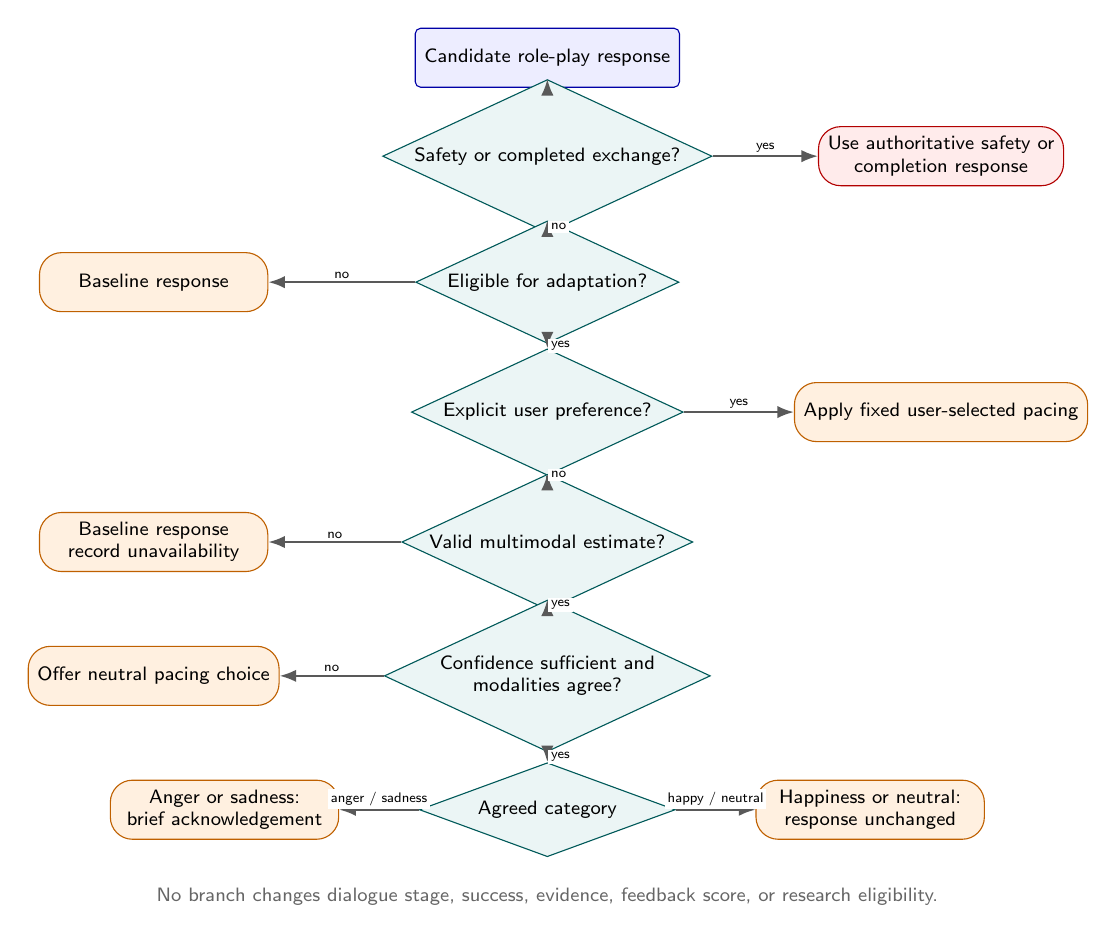
\begin{tikzpicture}[
    font=\sffamily\scriptsize,
    process/.style={draw=blue!65!black, fill=blue!7, rounded corners=2pt,
        align=center, minimum width=2.8cm, minimum height=0.75cm},
    decision/.style={diamond, draw=teal!70!black, fill=teal!8,
        aspect=2.15, align=center, inner sep=1.5pt, minimum width=3.25cm},
    action/.style={draw=orange!75!black, fill=orange!12, rounded corners=8pt,
        align=center, minimum width=2.9cm, minimum height=0.75cm},
    safety/.style={draw=red!70!black, fill=red!8, rounded corners=8pt,
        align=center, minimum width=2.9cm, minimum height=0.75cm},
    flow/.style={-{Latex[length=2.1mm]}, thick, draw=black!65},
    label/.style={font=\sffamily\tiny, fill=white, inner sep=1pt}
]
\node[process] (start) at (0,3.5) {Candidate role-play response};
\node[decision] (precedence) at (0,2.25) {Safety or completed exchange?};
\node[safety] (override) at (5.0,2.25) {Use authoritative safety or\\completion response};
\node[decision] (eligible) at (0,0.65) {Eligible for adaptation?};
\node[action] (baseline1) at (-5.0,0.65) {Baseline response};
\node[decision] (preference) at (0,-1.0) {Explicit user preference?};
\node[action] (manual) at (5.0,-1.0) {Apply fixed user-selected pacing};
\node[decision] (available) at (0,-2.65) {Valid multimodal estimate?};
\node[action] (baseline2) at (-5.0,-2.65) {Baseline response\\record unavailability};
\node[decision] (certain) at (0,-4.35) {Confidence sufficient and\\modalities agree?};
\node[action] (choice) at (-5.0,-4.35) {Offer neutral pacing choice};
\node[decision] (category) at (0,-6.05) {Agreed category};
\node[action] (ack) at (-4.1,-6.05) {Anger or sadness:\\brief acknowledgement};
\node[action] (unchanged) at (4.1,-6.05) {Happiness or neutral:\\response unchanged};

\draw[flow] (start)--(precedence);
\draw[flow] (precedence)--node[label, above]{yes}(override);
\draw[flow] (precedence)--node[label, right]{no}(eligible);
\draw[flow] (eligible)--node[label, above]{no}(baseline1);
\draw[flow] (eligible)--node[label, right]{yes}(preference);
\draw[flow] (preference)--node[label, above]{yes}(manual);
\draw[flow] (preference)--node[label, right]{no}(available);
\draw[flow] (available)--node[label, above]{no}(baseline2);
\draw[flow] (available)--node[label, right]{yes}(certain);
\draw[flow] (certain)--node[label, above]{no}(choice);
\draw[flow] (certain)--node[label, right]{yes}(category);
\draw[flow] (category)--node[label, above]{anger / sadness}(ack);
\draw[flow] (category)--node[label, above]{happy / neutral}(unchanged);

\node[align=center, text=black!60] at (0,-7.15)
    {No branch changes dialogue stage, success, evidence, feedback score, or research eligibility.};
\end{tikzpicture}
}
\caption{Decision tree for bounded affect-aware pacing. Every terminal action preserves the authoritative dialogue state and evidence.}
\label{fig:affect-policy}
\end{figure}

\subsection{Response Realisation}
\label{subsec:response-realisation}

Response realisation begins with the authoritative action and deterministic wording returned by the controller. In offline operation this wording is sent directly. When provider generation is enabled for a supported unbranched practice flow, the language model receives the saved scenario, difficulty behaviour, current role-play state, affect estimate, required action, and fallback wording. Its structured response must repeat the required action exactly, remain in character, avoid coaching and hidden-system language, and stay within a short response limit.

Failure to parse the response, an action mismatch, disallowed coaching language, an exception, or unavailable credentials returns the deterministic wording. For enhanced dialogue states containing a concrete constraint or proposal, even a plausible paraphrase is rejected unless it matches the authoritative wording; this conservative rule avoids treating a correct action label as evidence that a generated sentence preserved the negotiation facts. Branches likewise use deterministic wording so their differences arise from the participant's alternative response rather than an uncontrolled regeneration.

Outside role-play, the support-routing component described in Subsection~\ref{subsec:cognitive-support-routing} supplies one of the permitted general-response strategies. The response generator receives the selected strategy but cannot select it. Generation metadata records whether wording came from a template, deterministic role play, the provider, or a safety response, ensuring that later study summaries can count response sources and fallbacks without retaining provider internals.

\subsection{Safety Precedence and Crisis Interruption}
\label{subsec:safety-precedence}

A local crisis-language detector executes before model inference and response generation. Its bounded patterns cover direct self-harm and immediate-danger statements while applying exclusions for common negations, hypothetical or quoted material, and known false-positive phrases. When an external moderation service is configured, it can add a safety flag but cannot suppress a local match. This remains a conservative engineering safeguard rather than a validated clinical risk assessment.

On a detected safety condition, the backend skips multimodal inference and pacing, emits the fixed crisis response, and changes an active or paused role play to interrupted with the completion reason \texttt{safety\_interruption}. The decision trail preserves the preceding dialogue state and records the interruption action. Safety-interrupted wording is never reused as a suggested action-card phrase, and the research workflow does not count the attempt as a completed protocol task.

The response states the application's limitations and directs the user to emergency or crisis support without claiming to know the user's location or contacting services on their behalf. Because the deterministic safety path precedes provider and classifier output, failure of either optional component cannot remove the interruption. False negatives and ambiguous statements remain possible, which is why the interface consistently states that AffectLab is not monitored care, diagnosis, or emergency support.
%
\section{Feedback and Reflection Features}
\label{sec:feedback-reflection}

Feedback features are constructed from the evidence and decisions already stored during a rehearsal. They do not rerun an affect model, infer hidden reasoning, or ask a generator to judge the participant after completion. This design permits the user to move from a summary into the exact conversation evidence, try a bounded alternative, and prepare personal wording while preserving the original attempt.

\subsection{Evidence-Grounded Feedback Generation}
\label{subsec:evidence-feedback}

At completion, the role-play service calculates scenario-specific metrics from Boolean evidence attached to the participant's turns. Examples include clear request, specific evidence, maintained boundary, concise delivery, I-statements, and non-blaming language. A metric score is the proportion of relevant turns in which its condition was observed, and its evidence list contains the corresponding turn numbers. Versioned dialogue policies add stage-specific feedback while retaining the same link to stored evidence.

Deterministic templates turn these measurements into observed statements, strengths, and suggestions. A feature at or above the configured descriptive boundary becomes a strength; an absent or infrequent feature becomes a next-attempt suggestion. The completion reason and controller outcome remain separate from individual language metrics: reaching the turn limit is not relabelled as success, and a safety interruption is not scored as a skill failure. Custom scenarios receive metrics only for their selected supported skills.

If provider phrasing is enabled, it receives only the completed evidence-based feedback object and may reword its strengths and suggestions. The numeric scores, evidence links, and observations remain authoritative, and generation metadata distinguishes deterministic feedback from provider wording. Comparative feedback is added only when an earlier ordinary attempt uses the same scenario and scoring version; changes are described as differences in observed language rather than personal or clinical improvement.

\subsection{Conversation Replay}
\label{subsec:conversation-replay}

Replay is a read-only projection of the stored session rather than a second analysis pass. Its timeline is bounded by the role-play start and measurement-end timestamps, with a compatibility rule for older sessions that recorded only completion time. Later reflection is excluded, while reflection entered during a pause remains visible but has no controller decision and is not shown as a scored exchange. Missing boundaries, legacy decisions, unavailable feedback, and inference failures are displayed as gaps instead of being reconstructed.

Selecting an exchange highlights the paired user and assistant turns. Separate panels show observable language features, controller action and stage transition, generation source, and any saved affect-pacing decision. Technical details expose reason codes, before-and-after state, policy versions, modality distributions, confidence and agreement, availability, and timings. Feedback evidence buttons resolve stored evidence numbers back to their conversation-turn identifiers. Since exact phrase spans are unavailable, the complete source utterance is highlighted rather than presenting a guessed substring.

The browser constructs this view from the normal ownership-protected session response; replay has no new endpoint and makes no writes. It does not reload audio, regenerate explanations, or mutate recorded decisions. Navigation away from an unanswered immediate post-questionnaire may close that questionnaire window under the study rules, but inspection of the replay itself remains read-only.

\subsection{Rewind, Branching, and Comparison}
\label{subsec:rewind-branching}

Rewind removes only the most recent linked user--assistant rehearsal exchange. For versioned dialogue it restores the exact preceding snapshot, truncates the matching evidence and decision lists, clears completion and feedback, restores the previous affect state, and removes later research events. It is refused when the latest messages cannot be linked safely, when they belong to copied branch context, or after post-ratings or an explicit skip have fixed the measured attempt. The removed user text is returned to the composer for editing.

Branching provides a copy-on-write alternative without modifying the original. It is available only for completed or interrupted attempts whose stored policy and pre-turn snapshot are supported. The server validates ownership, source version, branch-point turn, linked decision, policy versions, and intact evidence. It then creates a deterministic child identifier from the user and request identifiers, copies only the context before the selected response, restores the saved pre-turn state, and records lineage including the parent version, copied turn identifiers, branch group, and SHA-256 digest of the source rehearsal.

The child is labelled as a retry with no required-study association. Its feedback covers only newly authored continuation evidence; copied context is not counted again in turn totals, events, or generation statistics. Comparison presents the shared context once and the original and alternative continuations side by side, including actions, evidence, sources, and outcomes. If the parent has been deleted, expired, or changed since the branch was created, the saved alternative remains usable but the original continuation is explicitly marked unavailable. This prevents a silently altered source from being presented as a controlled comparison.

Figure~\ref{fig:branching-model} illustrates the copy-on-write branch and the distinction between shared context and newly assessed continuation turns.

\begin{figure}[htbp]
\centering
\resizebox{\textwidth}{!}{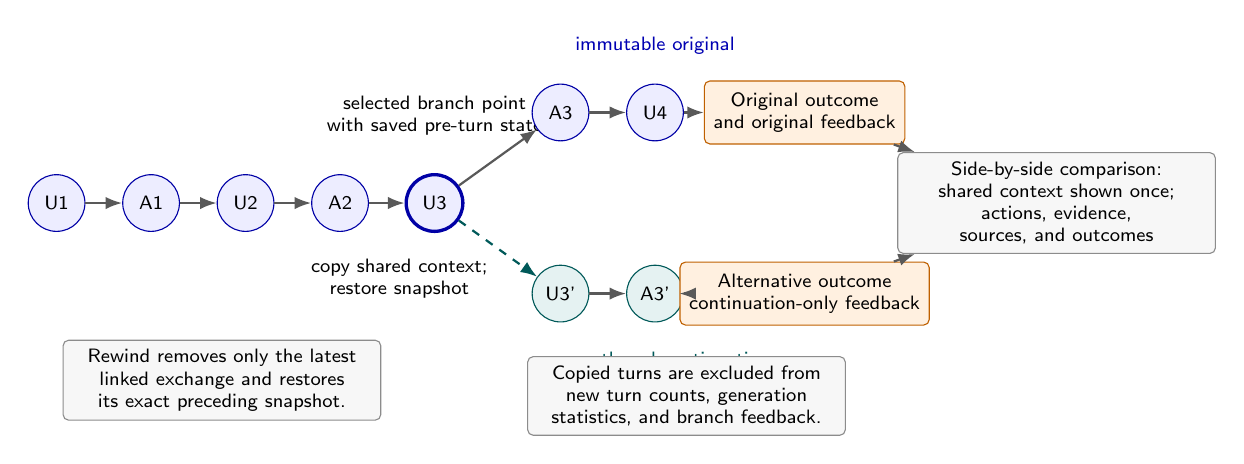
\begin{tikzpicture}[
    font=\sffamily\scriptsize,
    turn/.style={circle, draw=blue!65!black, fill=blue!7, minimum size=0.72cm,
        inner sep=1pt},
    branchturn/.style={circle, draw=teal!70!black, fill=teal!10, minimum size=0.72cm,
        inner sep=1pt},
    result/.style={draw=orange!75!black, fill=orange!12, rounded corners=2pt,
        align=center, minimum width=2.5cm, minimum height=0.8cm},
    note/.style={draw=black!45, fill=black!3, rounded corners=2pt,
        align=center, text width=3.8cm, minimum height=0.8cm},
    flow/.style={-{Latex[length=2.1mm]}, thick, draw=black!65},
    copied/.style={-{Latex[length=2.1mm]}, thick, dashed, draw=teal!70!black}
]
\node[turn] (u1) at (0,0) {U1};
\node[turn] (a1) at (1.2,0) {A1};
\node[turn] (u2) at (2.4,0) {U2};
\node[turn] (a2) at (3.6,0) {A2};
\node[turn, very thick] (point) at (4.8,0) {U3};
\draw[flow] (u1)--(a1); \draw[flow] (a1)--(u2); \draw[flow] (u2)--(a2); \draw[flow] (a2)--(point);
\node[above=0.35cm of point, align=center] {selected branch point\\with saved pre-turn state};

\node[turn] (oa) at (6.4,1.15) {A3};
\node[turn] (ou) at (7.6,1.15) {U4};
\node[result] (or) at (9.5,1.15) {Original outcome\\and original feedback};
\draw[flow] (point) -- (oa); \draw[flow] (oa)--(ou); \draw[flow] (ou)--(or);
\node[above=0.25cm of ou, text=blue!70!black] {immutable original};

\node[branchturn] (bu) at (6.4,-1.15) {U3'};
\node[branchturn] (ba) at (7.6,-1.15) {A3'};
\node[result] (br) at (9.5,-1.15) {Alternative outcome\\continuation-only feedback};
\draw[copied] (point) -- node[below left, align=center]{copy shared context;\\restore snapshot} (bu);
\draw[flow] (bu)--(ba); \draw[flow] (ba)--(br);
\node[below=0.25cm of ba, text=teal!70!black] {new authored continuation};

\node[note] (compare) at (12.7,0) {Side-by-side comparison:\\shared context shown once;\\actions, evidence, sources, and outcomes};
\draw[flow] (or)--(compare);
\draw[flow] (br)--(compare);

\node[note] at (2.1,-2.25) {Rewind removes only the latest linked exchange and restores its exact preceding snapshot.};
\node[note] at (8.0,-2.45) {Copied turns are excluded from new turn counts, generation statistics, and branch feedback.};
\end{tikzpicture}
}
\caption{Replay, rewind, and copy-on-write branching from a stored pre-turn dialogue snapshot.}
\label{fig:branching-model}
\end{figure}

\subsection{Takeaways and Action Cards}
\label{subsec:takeaways-action-cards}

The feedback screen provides a 500-character personal takeaway that is stored with the session and surfaced on the home dashboard. It is entirely user-authored and remains distinct from measured feedback. The dashboard also aggregates prior feedback metrics as a practice history, accompanied by language that these are averages of observed rehearsal features rather than a clinical assessment.

After a completed or interrupted rehearsal, the application can draft an action card containing an opening sentence, main request, boundary or fallback, and reminder. The draft draws only from eligible participant turns within the rehearsal measurement boundary and stores the identifiers of any reused source turns. It uses a maintained-boundary utterance where available, otherwise supplies neutral fallback wording. Safety-interrupted utterances and later reflection are excluded from suggested real-world phrasing.

The user can edit every card field before saving. Saving requires the expected session version, marks the card as user-edited, and updates neither feedback, questionnaires, research events, nor measurement boundaries. Cards can be copied or downloaded by the browser and survive normal session reloads. In a branch they use new continuation turns rather than silently recycling shared context, preserving the distinction between the original and alternative plans.
%
\section{Frontend Application}
\label{sec:frontend-application}

The frontend presents the backend's typed state as a sequence of participant and researcher workflows. It does not calculate authoritative dialogue transitions, affect decisions, or study completion in the browser. Instead, components retain editable local state, submit constrained requests, and replace their view with the version returned by the server. This keeps recovery behaviour and uncertainty disclosures as important as the successful path.

\subsection{Application Interface Overview}
\label{subsec:application-interface-overview}

Figures~\ref{fig:app-dashboard}, \ref{fig:app-roleplay}, and~\ref{fig:app-feedback} provide a compact visual overview of the participant-facing application. They follow the main user journey from choosing a practice activity, through an active rehearsal, to reviewing the resulting feedback. The screenshots should be captured with synthetic demonstration content and without personal or participant data. Only these three representative views are included because the purpose is to show the appearance and principal interactions of the implemented system, while the following subsections describe its behaviour in detail.

\begin{figure}[htbp]
    \centering
    \IfFileExists{figures/app-dashboard.png}{%
        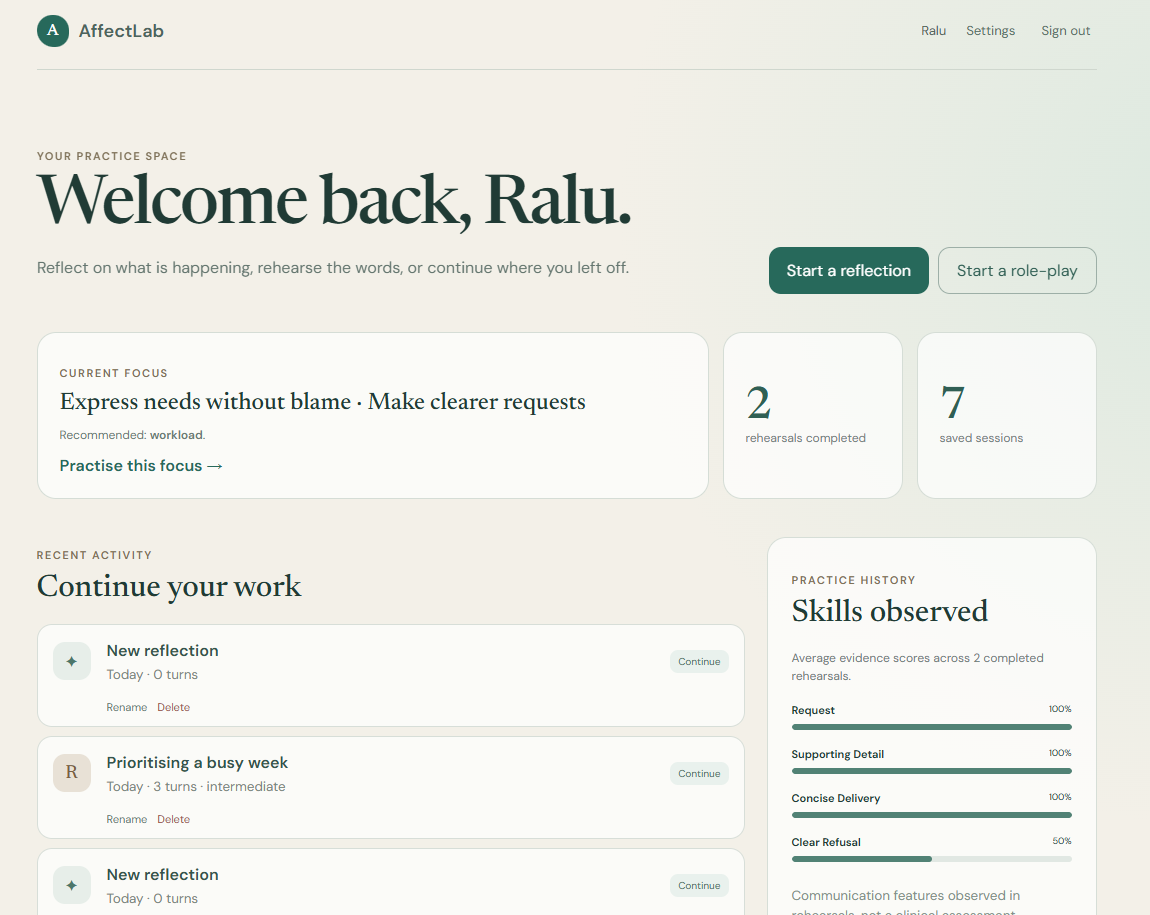
\includegraphics[width=\textwidth,height=0.68\textheight,keepaspectratio]{figures/app-dashboard.png}%
    }{%
        \fbox{\parbox[c][0.25\textheight][c]{0.92\textwidth}{\centering
        \textbf{Screenshot placeholder: home dashboard}\\[0.5em]
        Add \texttt{figures/app-dashboard.png}.}}
    }
    \caption{AffectLab home dashboard, showing the available practice paths, recommended starting point, and access to recent sessions and saved reflections.}
    \label{fig:app-dashboard}
\end{figure}

\begin{figure}[htbp]
    \centering
    \IfFileExists{figures/app-roleplay.png}{%
        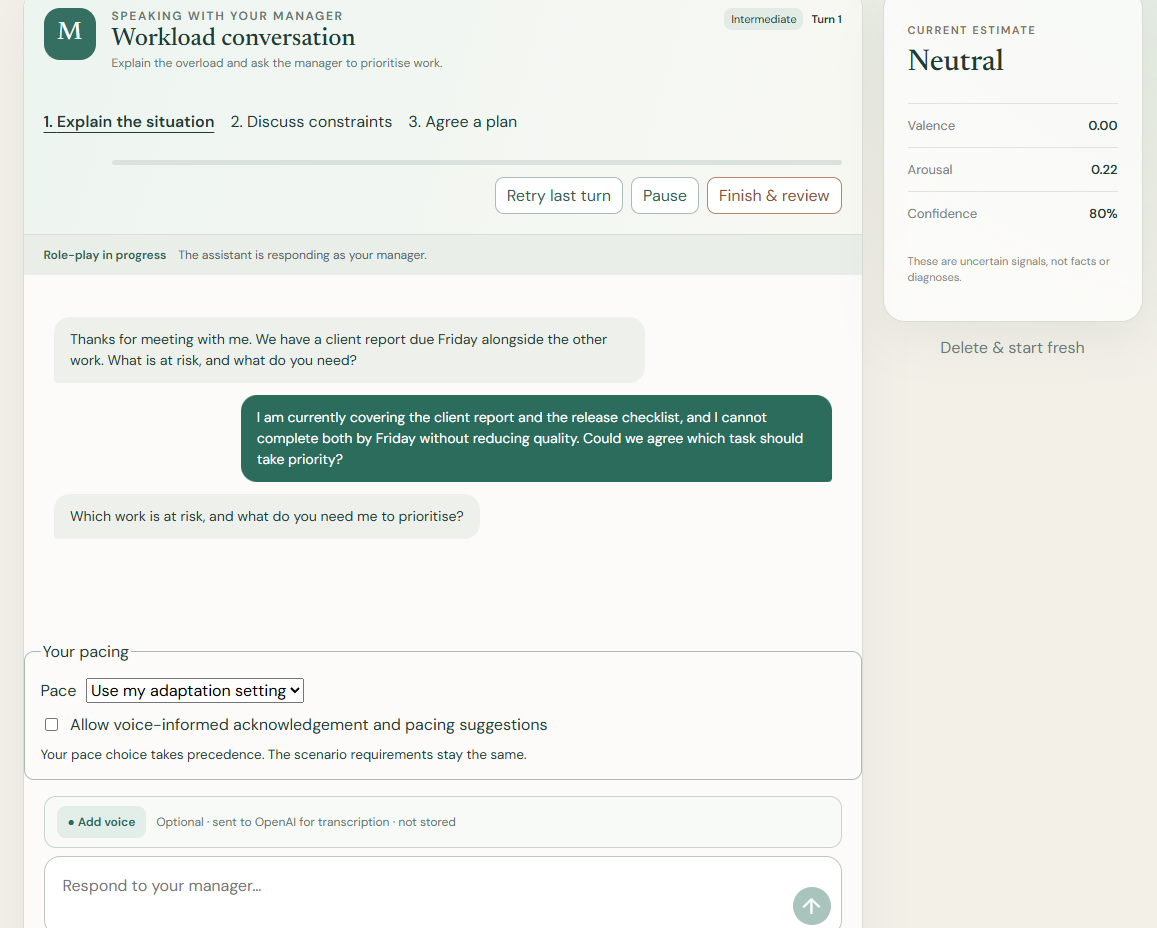
\includegraphics[width=\textwidth,height=0.68\textheight,keepaspectratio]{figures/app-roleplay.png}%
    }{%
        \fbox{\parbox[c][0.25\textheight][c]{0.92\textwidth}{\centering
        \textbf{Screenshot placeholder: role-play workspace}\\[0.5em]
        Add \texttt{figures/app-roleplay.png}.}}
    }
    \caption{Active role-play workspace, combining the conversation transcript and message composer with scenario progress, session controls, and optional voice and affect-aware functions. The standard affect panel shown here is the lexical estimate; a trained voice--text result, when available, appears in a separate panel.}
    \label{fig:app-roleplay}
\end{figure}

\begin{figure}[htbp]
    \centering
    \IfFileExists{figures/app-feedback.png}{%
        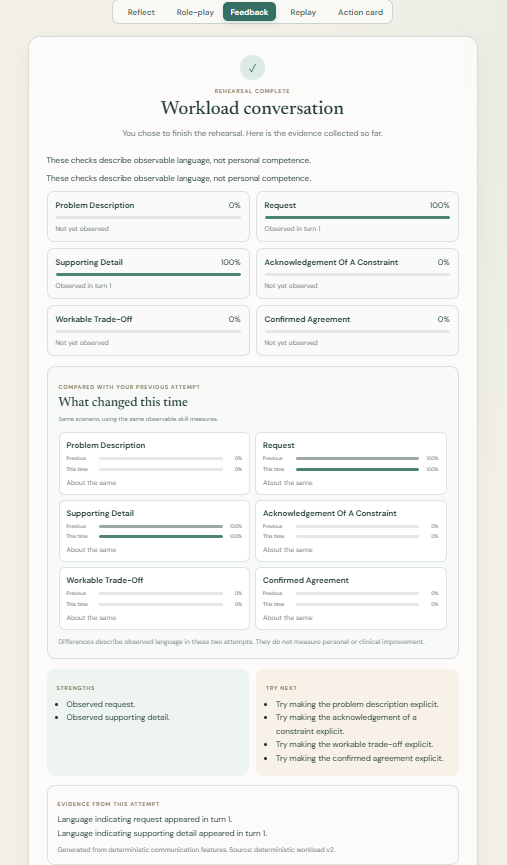
\includegraphics[width=\textwidth,height=0.68\textheight,keepaspectratio]{figures/app-feedback.png}%
    }{%
        \fbox{\parbox[c][0.25\textheight][c]{0.92\textwidth}{\centering
        \textbf{Screenshot placeholder: feedback and review}\\[0.5em]
        Add \texttt{figures/app-feedback.png}.}}
    }
    \caption{Post-rehearsal feedback and review interface, presenting evidence-linked observations and access to replay, alternative branches, personal takeaways, and the editable action card.}
    \label{fig:app-feedback}
\end{figure}

\subsection{Application Navigation and User Workflow}
\label{subsec:frontend-navigation}

The React application uses the browser History API to provide public landing and information pages, registration, sign-in, email verification and recovery, onboarding, the authenticated home dashboard, the practice workspace, settings, and the restricted researcher dashboard. On initial load it attempts to restore the access session and then performs one refresh-token exchange if necessary. Unauthenticated access to a protected route returns to sign-in, while a verified user who has not completed the current onboarding version is directed through onboarding before reaching the workspace.

Onboarding explains that the application is not therapy or diagnosis, that affect estimates can be wrong, that voice is optional, and that emergency support is outside the service. The user selects between one and three practice goals, which are stored on the account and used to recommend a starting scenario without restricting the available scenarios. The home dashboard then offers reflection, guided role play, recent sessions, saved takeaways, and a descriptive history of observed skills. Sessions can be resumed, renamed, or deleted.

The application shell includes explicit loading, empty, success, and failure states. An error boundary provides a recoverable sign-in path if a component cannot render. Network operations disable only the relevant control, expose errors through alert or status regions, and generally retain the user's input for retry. Responsive CSS changes the multi-column workspace and comparisons into single-column layouts, while visible keyboard focus, semantic controls, reduced-motion rules, live regions, and touch-sized actions support accessible desktop and mobile use.

\subsection{Conversation Preparation}
\label{subsec:frontend-preparation}

Participants can begin with a standard scenario or prepare a conversation in their own terms. The preparation form asks who the conversation is with, what happened, the desired outcome, and the difficult part. These answers are sent to the bounded preparation endpoint, which returns an editable scenario draft with an opening line, supported skills, and a tentative objection. The interface labels this output as a rehearsal plan rather than a prediction.

The participant reviews and may edit the title, character, situation, objective, opening line, expected skills, difficult part, and likely objection before saving the custom scenario. Validation errors remain attached to the draft so an outage or rejected save does not discard their work. Previously stored custom scenarios can be edited or deleted only through the account that owns them; older scenarios without preparation metadata remain compatible with the editor.

Before every attempt, the setup screen displays the selected character, objective, supported skill targets, difficulty description, and, where eligible, character profile. Pre-rehearsal confidence and anxiety ratings require an explicit complete response or an explicit skip. Starting from a populated session creates a new attempt rather than replacing prior reflection, feedback, or research history.

\subsection{Role-Play Workspace}
\label{subsec:frontend-roleplay-workspace}

The main workspace contains modes for reflection, active role play, feedback, replay, comparison, and the action card. A transcript panel presents ordered user and assistant turns, while the composer holds typed or reviewed transcribed text. During role play, a header shows the scenario, character, stage, progress, difficulty or profile, and controls for pause, resume, finish, and eligible rewind. Moving to reflection pauses an active rehearsal after confirmation; text entered while paused does not advance the role-play controller.

The browser includes the current session version and a newly generated request identifier with enhanced chat submissions. It clears the composer only after the server confirms the saved exchange. If a request fails, the typed draft and any voice attachment remain available; if the server reports a conflict, the interface offers to reload the committed conversation while retaining the draft. This avoids displaying a message bubble that was never persisted and lets the participant decide whether an uncertain submission should be sent again.

The workspace replaces its state from each response, including the saved user turn, assistant turn, emotion state, role-play status, feedback, and post-questionnaire opportunity. Busy indicators and an \texttt{aria-live} transcript communicate progress without inventing an optimistic response. Deleting and starting afresh requires a deliberate action and uses the backend deletion path rather than only clearing local display state.

\subsection{Voice Capture and Multimodal Interaction}
\label{subsec:frontend-voice}

Voice input is opt-in at both the settings and exchange levels. The browser requests microphone permission only after the participant selects the voice control, records for at most 20 seconds, and exposes recording and stop states. The captured signal is decoded through the browser audio context, mixed to mono, resampled to 16~kHz, encoded as PCM WAV, and kept only in component memory. Denied permission, unsupported recording, and conversion failure leave the text composer available.

When transcription is configured, stopping a recording sends the transient WAV to the authenticated transcription endpoint. The returned text is inserted into the composer for explicit review and editing; it does not become a conversation turn until Send is selected. A new recording or text edit clears any stale display associated with the previous draft. The reviewed text and optional WAV are then submitted together in one version-bound chat request so the affect estimate, pacing decision, and stored wording refer to the same exchange.

The interface permits a user to disable the microphone preference locally, enable automatic voice-informed pacing, or select keep going, gentler pace, or more challenge. It does not calculate predictions or send client-authored confidence values. After completion or failure, the component releases its media stream and object references. Raw audio is not added to browser session history or backend session objects.

\subsection{Presentation of Affect and Uncertainty}
\label{subsec:frontend-affect-presentation}

The standard emotion panel displays the backend's tentative lexical state using a distribution, valence, arousal, intensity, trend, and confidence. This is the panel shown in Figure~\ref{fig:app-roleplay}; it is not an output of the trained multimodal classifier. Its confidence is a deterministic heuristic derived from lexical evidence and temporal smoothing, so, for example, a displayed value of 80\% does not mean that the estimate has an empirically calibrated 80\% probability of being correct. Its language consistently presents these values as estimates. The panel is secondary to the conversation and is accompanied by the uncertainty disclaimer rather than being used as an authoritative description of how the user feels.

When a valid multimodal result is available, a separate panel presents the fused confidence, text and voice leaders, modality agreement, full distribution, latency, queue time, and the statement that audio was not stored. A fused label below the configured display threshold is headed as an uncertain estimate rather than as the predicted category. Disagreement receives an explicit explanation, and the full probabilities remain visible so that the leading label is not separated from its uncertainty.

For exchange-linked pacing, the ``Why this response?'' view uses the persisted \texttt{AffectDecision}. It shows whether analysis was requested and available, the selected action and reason, user preference, fallback code, model and policy versions, timings, and distributions. Reloading displays the same record and does not run inference again. Missing or failed inference is represented as an availability gap, not silently replaced by the lexical estimate.

Table~\ref{tab:application-analysis-components} makes explicit the different inputs, vocabularies, score semantics, operational effects, and supporting evidence of the four analysis and decision components. In particular, only the trained multimodal classifier has corpus-level classification and calibration evidence; the remaining scores expose deterministic rule strength or priority and must not be interpreted as probabilities.

\begin{table}[p]
\centering
\caption{Distinction between the trained affect model and the application's deterministic analysis and decision components.}
\label{tab:application-analysis-components}
\scriptsize
\begingroup
\setlength{\tabcolsep}{3pt}
\renewcommand{\arraystretch}{1.15}
\begin{tabularx}{\textwidth}{|>{\raggedright\arraybackslash}p{0.10\textwidth}|>{\raggedright\arraybackslash}p{0.11\textwidth}|>{\raggedright\arraybackslash}p{0.13\textwidth}|>{\raggedright\arraybackslash}X|>{\raggedright\arraybackslash}p{0.15\textwidth}|>{\raggedright\arraybackslash}p{0.16\textwidth}|}
\hline
\textbf{Component} & \textbf{Inputs} & \textbf{Labels or outputs} & \textbf{Meaning of scores} & \textbf{Affected behaviour} & \textbf{Evaluation evidence} \\ \hline
Trained multimodal classifier & Target text, up to three preceding causal turns, and up to 20 seconds of 16~kHz speech & Anger, happiness, neutral, and sadness & Temperature-scaled text and audio class probabilities followed by calibrated late fusion; confidence is the maximum fused probability & Separate voice--text panel and optional bounded pacing. It does not determine crisis handling and is excluded from required study tasks & Five speaker-independent IEMOCAP folds with classification, calibration, confusion-matrix, and dialogue-bootstrap analyses (Section~\ref{sec:multimodal-results}) \\ \hline
Lexical affect estimator (\texttt{lexical-v2}) & Current user text and the preceding lexical state used for smoothing & Anxiety, sadness, anger, frustration, shame, guilt, joy, and neutral; also valence, arousal, intensity, and trend & Normalised term weights, a neutral prior, punctuation adjustments, and temporal smoothing. Confidence is heuristic rule strength, not a calibrated probability & Standard affect panel; input to support-strategy selection and to bounded role-play state and evidence handling & Unit and authored-case tests of rule behaviour only; no labelled-corpus accuracy or calibration evaluation \\ \hline
Rule-based cognitive analyser & Current user text and the independently determined crisis flag & Five intent categories, ten possible cognitive-pattern matches, a possible cause, readiness, resistance, and request flags & Fixed values and pattern-derived weights indicating which rules matched; neither probabilities nor validated psychological measurements & Supplies tentative features to the strategy selector; it does not override crisis precedence or the role-play controller & Unit and integration cases described in Section~\ref{subsec:cognitive-routing-results}; no predictive- or construct-validity evaluation \\ \hline
Scored strategy selector & Smoothed lexical state and cognitive-analysis output & Validation, reflection, clarification, validate--reframe, practical suggestion, rehearsal invitation, de-escalation, or safety escalation & Additive rule priorities used to rank strategies; scores are not probabilities & Selects the general-response strategy outside active role play. Safety and active role-play actions remain independently authoritative & Deterministic policy and integration tests (Section~\ref{subsec:policy-case-results}); no evidence that the selected strategy is clinically effective or optimal \\ \hline
\end{tabularx}
\endgroup
\end{table}

\subsection{Feedback, Replay, and Comparison Interfaces}
\label{subsec:frontend-feedback-interfaces}

The feedback screen distinguishes the controller outcome from the individual metrics. It renders evidence scores, supporting turn numbers, strengths, suggestions, observed features, generation source, and any same-version comparison with a prior attempt. Difference labels explicitly refer to observed language in two rehearsals and avoid claims of personal improvement. The same screen hosts the personal takeaway and the immediate post-rehearsal ratings when their server-issued opportunity token is still valid.

Replay presents a selectable exchange timeline with linked evidence, controller state, generation provenance, and affect-pacing details. Buttons move focus to the source turn for keyboard as well as pointer users. Missing legacy data and unavailable measurement boundaries have dedicated explanations. From a supported user turn, the participant can create a branch; the original remains unchanged and the new workspace opens with copied context and the old response as an editable draft.

The comparison view separates shared context from two labelled continuation regions and stacks them on narrow screens. It reports utterances, evidence, actions, sources, outcomes, and agreements without ranking one branch as globally better. The action-card view provides editable, character-limited fields with save, retry, copy, and download controls. Save failures preserve edits, and version conflicts ask the user to refresh rather than overwriting a newer card.

\subsection{Optional Research Interfaces}
\label{subsec:frontend-research-interfaces}

Participant research controls live in settings and the authenticated dashboard rather than in public registration. The settings page fetches the current server-provided information sheet, displays eligibility criteria, data categories, processors, audio handling, retention, risks, withdrawal terms, and contacts, and requires separate confirmations plus the access code. Enrolled participants can see their pseudonymous identifier and consent versions, download a text-free personal research JSON file, or enter a two-step withdrawal flow without deleting the ordinary account.

An enrolled participant also receives a three-task checklist. It obtains progress from durable study records, labels tasks as not started, in progress, awaiting ratings, incomplete, or complete, and directs the next eligible action to workload, boundary, and relationship practice in order at intermediate difficulty. Required-task selection is fixed by the server; additional practice remains visibly separate. Closing or skipping a post-questionnaire advances the interface without calling the task complete.

The allow-listed researcher dashboard presents descriptive recruitment and completion counts, protocol status, scenario and difficulty summaries, questionnaire averages, skill summaries, generation sources, and pseudonymous participant activity. Researchers may set the collection dates, record a bounded exclusion reason and data-quality note, download the versioned CSV, and initiate the final dataset freeze when eligible. Names, email addresses, transcripts, audio, custom wording, and takeaways are not rendered. A non-researcher cannot reach this view merely by navigating to its route because the API applies the independent researcher dependency.
%
\section{Optional Research Support and Data Export}
\label{sec:research-workflow-implementation}

The research workflow implements the frozen feasibility protocol as versioned application state. Account privacy acceptance and study participation are separate, and ordinary use of AffectLab does not imply research consent. The protocol identifier, consent version, eligibility version, attempt purpose, task association, and measurement timestamps are carried into the records needed to reconstruct the study flow.

\subsection{Participant Enrolment and Consent}
\label{subsec:participant-enrolment}

The participant information endpoint supplies the current study title, protocol and consent versions, eligibility scope, collected data, external processors, audio handling, retention statement, risks, limitations, withdrawal terms, and research contacts. Enrolment requires an authenticated, verified account, a configured access code, an open collection window, and explicit confirmation that the information was read, participation is voluntary, and the stated processing is accepted. The access code is compared using a constant-time operation.

Eligibility is confirmed separately for minimum age, approved geography, English use, and the additional frozen inclusion and exclusion criteria. The backend stores the criteria fingerprint, protocol version, and confirmation time, but not date of birth, precise address, health details, or a reason for ineligibility. If the configured criteria, consent version, or protocol changes, the old confirmation is not silently treated as current. Withdrawn or researcher-excluded accounts cannot re-enrol, and enrolment closes once dataset freezing begins.

Successful enrolment creates a pseudonymous participant identifier independent of email and records the exact consent and eligibility versions. These fields are evaluated again when starting a required task or accessing progress; possession of an access token from an earlier state is insufficient. The protocol is a single-arm feasibility and usability pilot, and the application does not expose efficacy or clinical-effectiveness claims.

\paragraph{Pilot evaluation boundary.} Required study tasks are deliberately ineligible for multimodal inference and affect-aware pacing, as specified by the request-processing eligibility check and the adaptation policy in Subsection~\ref{subsec:affect-pacing}. The pilot therefore evaluates completion and perceptions of the baseline text-based rehearsal and deterministic feedback workflow. Its post-task realism and usefulness ratings do not evaluate, and cannot support claims about, the acceptability or benefit of the emotion-aware adaptation itself. Multimodal model quality and adaptation-policy behaviour are instead evaluated through the separate benchmark experiments and engineering tests reported in Chapter~\ref{chap5}.

\subsection{Study Progress and Questionnaires}
\label{subsec:study-progress-questionnaires}

The required procedure contains workload, boundary, and relationship scenarios in that order, each at intermediate difficulty and on the non-adaptive baseline path. Only an attempt explicitly marked required and associated with the matching scenario can become the primary attempt for a task. The first such attempt is selected deterministically by start time and session identifier; an additional practice, retry, custom scenario, branch, or later successful attempt cannot replace it. This prevents optional affect-aware practice from entering the pilot outcomes and prevents outcome-driven reassignment of the protocol record.

Before an attempt begins, confidence and anxiety use integer ratings from 1 to 7. After an eligible completed rehearsal, confidence, realism, and usefulness use the same scale. Each phase requires either all declared items or an explicit skip. Pre-ratings cannot be added after the role play starts, and post-ratings require the one-use token issued at completion. Leaving the immediate feedback opportunity closes it; a saved response or skip cannot be edited, and the attempt cannot then be rewound.

A required task is complete only when the required scenario and difficulty match, its completion reason is success, maximum turns, or manual finish, and a complete post-questionnaire exists. A safety interruption, omitted post-ratings, closed window, or abandoned task remains incomplete. Progress nevertheless permits the participant to continue to later tasks, preserving observable missingness rather than forcing or fabricating a score. Collection dates and dataset-freeze state can disable new required activity while leaving ordinary practice available.

\subsection{Pseudonymous Research Records}
\label{subsec:pseudonymous-records}

Eligible post-consent session activity is projected into a separate \texttt{StudyRecord}. It contains participant and session pseudonyms, protocol and consent versions, enrolment and activity times, retention deadline, turn count, attempt and branch classification, scenario, difficulty, completion reason, measurement times, numeric feedback metrics, questionnaire values, generation and fallback counts, and text-minimised event records. Pre-consent events are excluded, and branch copies are not counted as new participant activity.

The record excludes account names, email, password material, conversation text, raw audio, custom scenario wording, feedback prose, saved takeaways, action cards, and dialogue snapshots. Event export further reduces properties to counts because even a nominally structured property could contain custom wording. A participant with no retained sessions still receives a participant-level export row so the enrolment denominator is not silently reduced.

Study-record retention is independent of the shorter application-session lifecycle. Each eligible activity refreshes the configured research deadline, and MongoDB applies a separate time-to-live index. Startup backfilling projects missing records only for currently eligible, post-consent material. A protocol freeze blocks further durable study-record changes, preserving the final analysis boundary.

\subsection{Research Dashboard and Data Export}
\label{subsec:research-dashboard-export}

The researcher dashboard constructs aggregates from the current protocol cohort while excluding withdrawn and researcher-excluded participants from analysis. It reports enrolment and completer targets, protocol completion, completed rehearsals, scenario and difficulty counts, questionnaire averages, deterministic skill averages, generation sources, and participant-level lifecycle status. These are descriptive monitoring values; the inferential analyses and substantive results belong to Chapter~\ref{chap5}.

The live CSV uses the versioned \texttt{affectlab-frozen-dataset-v4} schema. Its rows include pseudonymous identifiers, consent and eligibility versions, timestamps, task classification, branch and feedback scope, questionnaire values, numeric feedback, generation and fallback counts, and event counts. Missing values remain empty rather than imputed. Branch rows explicitly report copied-context counts and continuation-only feedback so that they are not pooled unknowingly with full attempts. The participant's personal JSON export follows the same exclusion of identity and conversation text while retaining their own participant identifier.

Once the configured study end date is reached, an authorised researcher may start the freeze operation. The repository uses a freeze token to prevent concurrent freezes, generates a de-identified CSV with new sequential participant and session labels, stores its schema, protocol, time, row and participant counts, and SHA-256 digest, and then marks the lifecycle frozen. Subsequent CSV downloads return this immutable stored content with its checksum. Date changes, participant-review edits, enrolment, and research-record updates are blocked after freezing; withdrawal remains available, although an irreversibly de-identified frozen row can no longer be linked for removal.

Figure~\ref{fig:research-data-lifecycle} summarises the minimising projection, distinct retention domains, and boundary introduced by irreversible dataset freezing.

\begin{figure}[htbp]
\centering
\resizebox{\textwidth}{!}{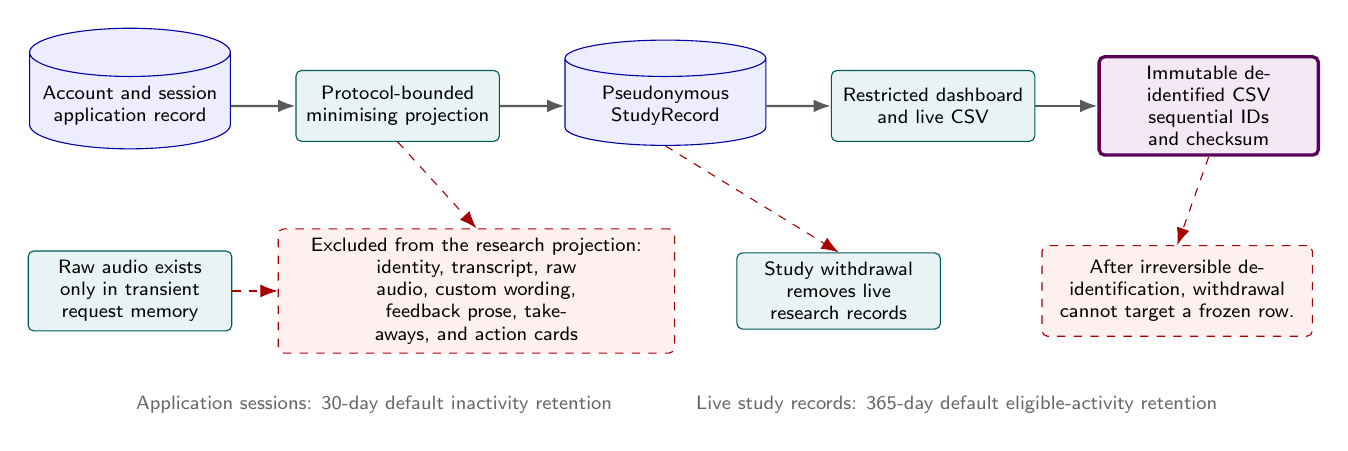
\begin{tikzpicture}[
    font=\sffamily\scriptsize,
    store/.style={cylinder, shape border rotate=90, aspect=0.25,
        draw=blue!65!black, fill=blue!7, align=center,
        minimum width=2.55cm, minimum height=1.05cm},
    process/.style={draw=teal!70!black, fill=teal!9, rounded corners=2pt,
        align=center, text width=2.35cm, minimum height=0.9cm},
    frozen/.style={draw=violet!70!black, fill=violet!9, very thick, rounded corners=2pt,
        align=center, text width=2.55cm, minimum height=0.95cm},
    exclude/.style={draw=red!65!black, fill=red!6, dashed, rounded corners=2pt,
        align=center, text width=4.8cm, minimum height=1.15cm},
    flow/.style={-{Latex[length=2.2mm]}, thick, draw=black!65},
    remove/.style={-{Latex[length=2.2mm]}, dashed, draw=red!65!black}
]
\node[store] (account) at (0,0.8) {Account and session\\application record};
\node[process] (projection) at (3.4,0.8) {Protocol-bounded minimising projection};
\node[store] (study) at (6.8,0.8) {Pseudonymous\\StudyRecord};
\node[process] (live) at (10.2,0.8) {Restricted dashboard and live CSV};
\node[frozen] (freeze) at (13.7,0.8) {Immutable de-identified CSV\\sequential IDs and checksum};

\draw[flow] (account)--(projection);
\draw[flow] (projection)--(study);
\draw[flow] (study)--(live);
\draw[flow] (live)--(freeze);

\node[process] (audio) at (0,-1.55) {Raw audio exists only in transient request memory};
\node[exclude] (excluded) at (4.4,-1.55) {Excluded from the research projection:\\identity, transcript, raw audio, custom wording,\\feedback prose, takeaways, and action cards};
\node[process] (withdraw) at (9.0,-1.55) {Study withdrawal removes live research records};
\node[exclude, text width=3.2cm] (limit) at (13.3,-1.55)
    {After irreversible de-identification, withdrawal cannot target a frozen row.};

\draw[remove] (audio)--(excluded);
\draw[remove] (projection.south)--(excluded.north);
\draw[remove] (study.south)--(withdraw.north);
\draw[remove] (freeze.south)--(limit.north);

\node[align=center, text=black!60] at (3.1,-3.0)
    {Application sessions: 30-day default inactivity retention};
\node[align=center, text=black!60] at (10.5,-3.0)
    {Live study records: 365-day default eligible-activity retention};
\end{tikzpicture}
}
\caption{Research-data lifecycle from the richer account-owned session to the pseudonymous live record and immutable de-identified export.}
\label{fig:research-data-lifecycle}
\end{figure}
%
\section{Security, Privacy, and Data Protection}
\label{sec:security-privacy-data-protection}

Security and privacy controls are distributed across configuration validation, middleware, authentication services, ownership-aware repositories, data minimisation, and user-facing lifecycle operations. They establish a production-oriented security baseline rather than a guarantee of confidentiality. The repository includes a separate remote-deployment baseline because a local demonstration configuration is not sufficient for internet-facing use.

\subsection{Authentication and Token Management}
\label{subsec:security-token-management}

Account passwords are accepted only over the API's protected transport boundary in a deployed environment and are converted immediately to recommended adaptive hashes. Verification and password-reset values are generated with a cryptographic random source; the database receives only SHA-256 digests and expiry times. Password reset validates the new password before atomically consuming the stored record, so an invalid new password does not destroy the recovery opportunity while two successful requests cannot reuse it.

Access tokens are signed, typed JSON Web Tokens with configurable short lifetimes. Refresh tokens have separate type claims and unique identifiers, and their digests permit server-side rotation and revocation. The browser keeps the access token in session storage, whereas the refresh credential is an HTTP-only, same-site cookie restricted to the authentication path and marked secure in production. Changing or resetting a password revokes all refresh records and signs the current browser out.

Generic registration, verification-resend, and password-recovery responses reduce account enumeration. Email verification is checked after reloading the user on protected requests. Authentication and email endpoints have dedicated rate-limit categories, and production start-up rejects a disabled limiter. These controls reduce common automated misuse but do not replace monitoring, secret rotation, or infrastructure-level abuse protection.

\subsection{Authorisation and Resource Isolation}
\label{subsec:authorisation-isolation}

Authorisation begins with the authenticated account identifier and is repeated at the persistence boundary. Session read, list, update, delete, multimodal analysis, branching, comparison, questionnaire, feedback, and action-card operations all obtain the session through an identifier-and-owner query. An unauthorised identifier produces the same not-found behaviour as a missing session. Custom scenarios are nested in the owning user, and branch creation verifies both parent and child lineage against that owner.

Researcher authorisation is not inferred from a route, client flag, or pilot enrolment. It requires a verified account whose normalised email is present in the server-side allow-list. Study operations additionally check current consent, eligibility version, protocol version, withdrawal and exclusion state, collection dates, and freeze state. Dataset lifecycle mutations, participant review, and exports therefore remain protected even if a participant manually invokes their URLs.

Optimistic versions and idempotency identifiers add integrity protection to authorisation. They do not merely identify who may write, but also which state that write was based on. Conditional MongoDB replacements and deterministic branch identifiers prevent lost updates and duplicate alternatives across processes. The API returns conflicts for recovery instead of choosing a winner silently.

\subsection{Audio and Conversation Data Handling}
\label{subsec:audio-conversation-data}

Conversation text is stored because session continuation, replay, evidence links, and deletion controls require it. When provider-backed generation is enabled, the relevant session context may be sent to the configured provider with response storage disabled. The application does not write raw prompts or generated replies to its own operational logs. The participant information and settings interfaces disclose these boundaries rather than treating local and provider processing as equivalent.

Audio requires an explicit recording action for every exchange. The browser holds the WAV transiently, and the backend checks encoded and decoded size, file structure, duration, channels, and sample rate before transcription or local inference. Transcription may send it to the configured provider, whereas multimodal inference processes it in memory. Neither path adds the recording to the session, study record, or export. Only an approved transcript, bounded prediction summary, provenance, and pacing decision may persist.

Research projections minimise the richer session document. They omit identity, transcripts, free-text feedback, custom scenario content, takeaways, action cards, and raw model inputs. Exported event information is counted by event name rather than exposing arbitrary properties. Source-control exclusions separately keep environment files, local databases, raw datasets, checkpoints, model artefacts, generated runs, and backup material outside the repository.

\subsection{Retention, Withdrawal, and Account Deletion}
\label{subsec:retention-deletion}

Application sessions and research records have distinct retention fields. By default, an active session expires after 30 days of inactivity, while a pseudonymous study record expires 365 days after its latest eligible activity. MongoDB time-to-live indexes perform eventual physical deletion, and repository reads also apply the deadlines logically so expired material is not returned while background deletion is pending. Token collections use their own expiry indexes.

A participant may delete an individual session without deleting the account. Account deletion removes the user, owned sessions, live study records, refresh tokens, and outstanding verification and reset records. The settings interface requires browser confirmation and retains the signed-in state if the request fails, allowing a safe retry. Backups remain a separate operational responsibility and must follow the approved encrypted retention schedule.

Study withdrawal is intentionally narrower. It removes questionnaires, questionnaire skips, post-rating tokens, research-event telemetry, and live study records, and marks the account as withdrawn so it is excluded from later collection and export. Ordinary account access, conversations, feedback, and takeaways remain available. The interface explains that rows already irreversibly de-identified in a frozen export or incorporated into aggregate analysis may no longer be linkable for removal. Re-enrolment after withdrawal is blocked.

\subsection{Deployment Security Controls}
\label{subsec:deployment-security-controls}

Setting the environment to production, pilot, or staging activates fail-fast configuration validation. The signing secret must be unique and at least 32 bytes; allowed origins must be explicit HTTPS addresses; trusted hosts cannot contain a wildcard; HTTPS enforcement and rate limiting must be enabled; and offline demonstration mode is prohibited. Refresh cookies become secure and responses add HTTP Strict Transport Security. CORS still permits credentials only from the declared origins.

The API and Nginx layers add complementary content-security, framing, referrer, content-type, permissions, and caching headers. Host validation and HTTPS redirection occur in the backend, while the frontend server restricts executable and embedded sources and grants media access only to local blob content. The intended remote arrangement terminates TLS at a maintained reverse proxy and prevents direct public access to MongoDB and the application server.

The bundled limiter is explicitly scoped to a single backend process and does not trust forwarded client-address headers. A multi-worker deployment must use a shared gateway or distributed limiter. The operational baseline also requires patched hosts, dependency auditing, protected secrets, encrypted access-controlled backups, and a restore drill. The backup utility preserves BSON types and indexes, records per-collection checksums and counts, and will restore by default only into an empty database whose name ends in \texttt{\_restore\_test}, reducing the chance of overwriting the live store.
%
\section{Deployment and Configuration}
\label{sec:deployment-configuration}

The implementation supports three related execution arrangements: direct local development, a containerised integrated stack, and a deliberately offline demonstration. These arrangements reuse the same application code but select different repositories and optional services through configuration. None embeds production credentials or private model files in an image.

\subsection{Local and Containerised Deployment}
\label{subsec:local-container-deployment}

For local development, MongoDB can run as an existing service while Uvicorn serves the FastAPI application and Vite serves the frontend with hot reloading. The API address is provided to the frontend at build or development time. Developers may instead select the in-memory repository for isolated service work, accepting that its contents disappear when the process stops.

Docker Compose defines MongoDB 8, the backend, and the production frontend. A named volume stores database contents, the backend waits for the MongoDB health check, and the frontend waits for backend readiness. The backend image installs the core requirements into a Python 3.12 slim base and runs Uvicorn. Optional PyTorch and Transformers packages and private model directories are deliberately absent unless a separate inference-capable deployment supplies them.

The frontend uses a Node.js 22 build stage to run the TypeScript and Vite production build, then copies only compiled assets into an Nginx image. Nginx serves the single-page-application fallback, prevents caching of \texttt{index.html}, applies immutable caching to content-hashed assets, and exposes a small health endpoint. Compose's default values are for local use; a remote deployment must replace the development signing secret and satisfy all production validation.

Figure~\ref{fig:deployment-topology} shows the resulting service topology and distinguishes locally controlled components from optional external processing.

\begin{figure}[htbp]
\centering
\resizebox{\textwidth}{!}{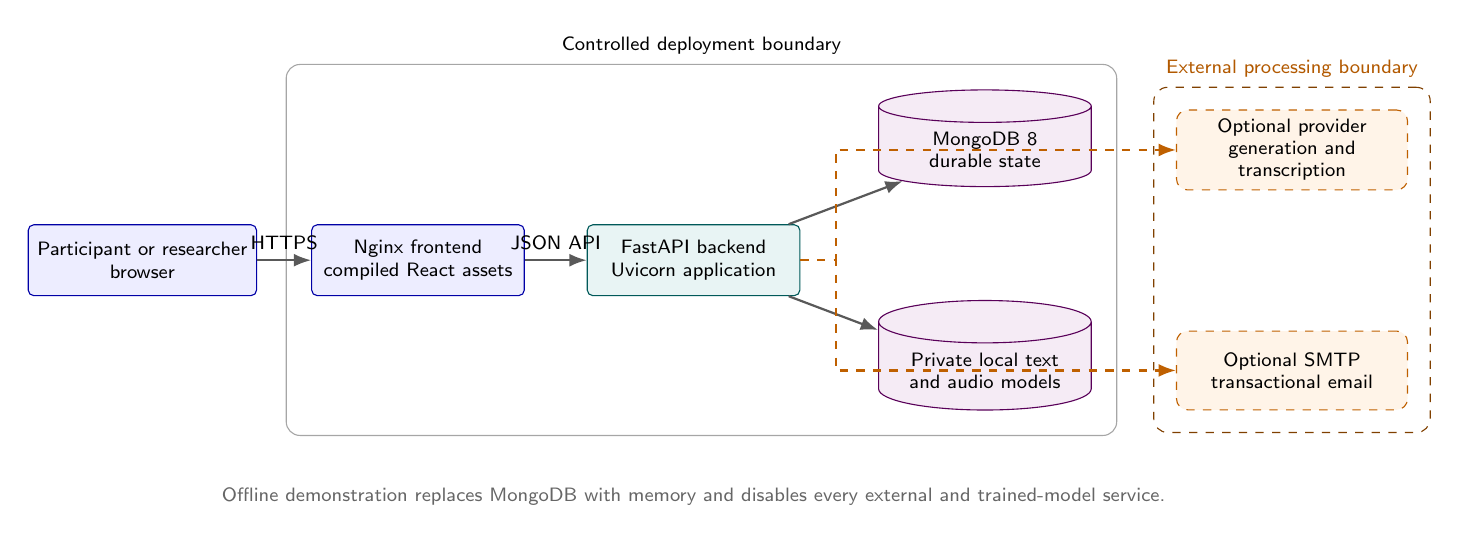
\begin{tikzpicture}[
    font=\sffamily\scriptsize,
    nodebox/.style={draw=blue!65!black, fill=blue!7, rounded corners=2pt,
        align=center, minimum width=2.7cm, minimum height=0.9cm},
    service/.style={draw=teal!70!black, fill=teal!9, rounded corners=2pt,
        align=center, minimum width=2.7cm, minimum height=0.9cm},
    store/.style={cylinder, shape border rotate=90, aspect=0.25,
        draw=violet!70!black, fill=violet!8, align=center,
        minimum width=2.7cm, minimum height=1.0cm},
    external/.style={draw=orange!75!black, fill=orange!9, dashed,
        rounded corners=4pt, align=center, text width=2.7cm,
        minimum height=1.0cm},
    flow/.style={-{Latex[length=2.2mm]}, thick, draw=black!65},
    optional/.style={-{Latex[length=2.2mm]}, dashed, thick, draw=orange!75!black}
]
\node[nodebox] (browser) at (0,0) {Participant or researcher\\browser};
\node[nodebox] (nginx) at (3.5,0) {Nginx frontend\\compiled React assets};
\node[service] (api) at (7.0,0) {FastAPI backend\\Uvicorn application};
\node[store] (mongo) at (10.7,1.4) {MongoDB 8\\durable state};
\node[store] (models) at (10.7,-1.4) {Private local text\\and audio models};
\node[external] (provider) at (14.6,1.4) {Optional provider\\generation and transcription};
\node[external] (smtp) at (14.6,-1.4) {Optional SMTP\\transactional email};

\draw[flow] (browser)--node[above]{HTTPS}(nginx);
\draw[flow] (nginx)--node[above]{JSON API}(api);
\draw[flow] (api)--(mongo);
\draw[flow] (api)--(models);
\draw[optional] (api.east)--++(0.45,0) |- (provider.west);
\draw[optional] (api.east)--++(0.45,0) |- (smtp.west);

\begin{scope}[on background layer]
  \node[fit=(nginx)(api)(mongo)(models), draw=black!35, rounded corners=5pt,
      inner sep=9pt, label={[font=\sffamily\scriptsize]above:Controlled deployment boundary}] {};
  \node[fit=(provider)(smtp), draw=orange!50!black, dashed, rounded corners=5pt,
      inner sep=8pt, label={[font=\sffamily\scriptsize, text=orange!70!black]above:External processing boundary}] {};
\end{scope}

\node[align=center, text=black!60] at (7.0,-3.0)
    {Offline demonstration replaces MongoDB with memory and disables every external and trained-model service.};
\end{tikzpicture}
}
\caption{Containerised deployment topology and external-service boundary.}
\label{fig:deployment-topology}
\end{figure}

\subsection{Offline Demonstration Mode}
\label{subsec:offline-demo}

The offline configuration selects the in-memory repository, creates a verified demonstration account at application startup, and disables OpenAI generation, role-play generation, transcription, multimodal inference, SMTP, and rate limiting. Reflection and rehearsal therefore use only deterministic local templates. No MongoDB, cloud storage, private model, email server, or internet connection is required.

This mode makes the application's graceful-degradation claims demonstrable without pretending that unavailable capabilities ran. Model and transcription status remain unavailable, and data disappear on backend restart. The configuration validator rejects offline demonstration in production-like environments, so convenience credentials and automatic account creation cannot be enabled accidentally for a remote pilot.

A synthetic demonstration dataset and runbook keep example conversation content separate from participant data. A stronger engineering demonstration uses real MongoDB and a compiled frontend but still disables external providers and trained inference. The two modes serve different purposes: the memory-backed mode is portable for presentation, while the isolated MongoDB smoke run verifies persistence and restart behaviour.

\subsection{Environment-Based Configuration}
\label{subsec:environment-configuration}

Settings can be supplied through process variables or repository- and backend-level environment files. They cover API origins and hosts, repository choice and database name, token and retention lifetimes, provider models and timeouts, SMTP, multimodal paths and thresholds, consent and protocol versions, study targets and contacts, eligibility scope, researcher allow-list, access code, offline credentials, and rate limits. Defaults support development but do not silently qualify as production settings.

The checked-in example file documents required names without containing live secrets. The real \texttt{.env} file is ignored by version control. Private model weights are synchronised into a user-selected local directory and referenced by path; raw IEMOCAP data and derived row-level artefacts remain outside the application repository. Separate dependency sets allow a deployment to omit local machine-learning libraries entirely.

Configuration values with scientific meaning are also retained in versioned JSON rather than only in mutable environment variables. These include the final multimodal label order, input limits and calibration chain, as well as the study protocol task order, measures, missing-data policy, target sizes, and prohibition on efficacy claims. This separates deployer-specific secrets from inspectable experimental decisions.

\subsection{Health Checks and Operational Failure Handling}
\label{subsec:health-failure-handling}

The liveness endpoint reports only that the API process can respond. Readiness revalidates settings, pings the repository, and verifies every required index; configuration, persistence, and index failures receive distinct states and HTTP 503. Optional transcription and multimodal capabilities are reported separately and do not make the text-first service unready. Container health checks consume these endpoints for dependency ordering and restart decisions.

Expected failures are translated into bounded client responses: unauthenticated and forbidden requests, missing resources, validation failures, unavailable optional services, rate limits with \texttt{Retry-After}, and concurrency conflicts have distinct status codes. Provider exceptions and inference failures do not expose stack traces or raw exception content in conversation records. The frontend preserves drafts and presents retry or reload actions according to whether the operation may have committed.

The system is designed to fail closed where authority is involved and fail soft where an enhancement is involved. Missing ownership, stale state, invalid consent, a closed study window, or a dataset freeze prevents the write. Missing generation, transcription, or emotion-model capability preserves the deterministic text workflow. This distinction keeps availability from weakening access, protocol, or safety constraints.
%
\section{Implementation Verification}
\label{sec:implementation-verification}

Verification is organised by boundary rather than by a single undifferentiated test suite. Deterministic unit tests check policies and transformations, API tests check contracts and ownership, MongoDB tests check real persistence semantics, browser tests check user workflows and accessibility, performance tests detect latency regressions, and smoke tests join the compiled components. These developer-led checks provide the principal evidence for application quality; model accuracy and supplementary user perceptions remain separate questions.

\subsection{Backend Unit and Integration Testing}
\label{subsec:backend-testing}

The default pytest suite forces the in-memory repository and disables SMTP, provider, transcription, and trained-model inference. It tests authentication and recovery, generic anti-enumeration responses, token rotation and revocation, ownership, optimistic versions, session lifecycle, study consent and questionnaires, exports and freezing, preparation, feedback, replay boundaries, rewind, branching, crisis precedence, dialogue transitions, affect pacing, and optional-service failure. Parameterised cases exercise profiles, difficulty levels, negations, reversals, confidence combinations, missing modalities, duplicate requests, and legacy compatibility.

Machine-learning support tests separately validate IEMOCAP parsing, safe archive paths, causal context, speaker-independent folds, class weights, calibration, probability metrics, utterance pairing, fusion, bootstrap procedures, and balanced final-model smoke selection. The disabled multimodal service is tested without importing heavy machine-learning dependencies; concurrency tests verify serial inference access when enabled. These fixtures confirm implementation contracts, not the accuracy of a trained model on new users.

MongoDB integration tests are opt-in and create uniquely named disposable databases. They recreate repository and service clients to check persistence across restart, required indexes and logical expiry, separate study retention, cascade deletion, optimistic conflict detection, single-use recovery, versioned dialogue restoration, branch idempotency, and saved affect provenance. Backup tests create an archive, restore it into a protected disposable target, and compare checksums and document counts.

Ruff checks imports, syntax-level errors, modern Python usage, and selected bug patterns across application, test, and script code. Dependency security is checked separately because style and behavioural tests cannot identify published package vulnerabilities.

\subsection{Frontend End-to-End Testing}
\label{subsec:frontend-testing}

The regular Playwright suite runs the browser against a deterministic mocked API boundary. This makes UI state and failure injection repeatable while testing registration and onboarding, required and ordinary practice, preparation, voice-review submission, feedback, replay, branching, comparison, action cards, research enrolment, questionnaire timing, researcher access, settings, and account recovery. Dedicated cases abort or reject network calls to verify that drafts, recordings, selections, and stored rows are not falsely discarded.

Projects run in desktop Chromium and a mobile Chromium profile. Representative pages are scanned with axe-core against WCAG 2.0 and 2.1 A/AA rule sets, alongside assertions for keyboard focus, accessible names, live status messages, and responsive layouts. Production compilation runs the strict TypeScript project build before Vite bundling, and ESLint checks React hook and TypeScript rules.

Because the normal browser suite mocks the backend, its passing result demonstrates frontend behaviour against declared contracts rather than integrated persistence. Assertions that depend on real authentication, FastAPI serialisation, MongoDB indexes, or process restart are reserved for the full-stack suite.

\subsection{Performance Regression Testing}
\label{subsec:performance-testing}

The repeatable performance script exercises the deterministic text-first workflow through FastAPI's in-process HTTP test transport. After warming the application, it records repeated liveness, authenticated scenario-catalogue, session-creation, role-play-start, and conversation-turn requests. Each summary includes the sample count, median, 95th percentile, and maximum, while the evidence file records the execution environment and SHA-256 hashes of the relevant application and benchmark sources.

The benchmark deliberately uses the memory repository and disables transcription, trained multimodal inference, and provider generation. This isolates locally controlled routing, authentication, validation, dialogue, persistence-interface, and serialisation overhead and makes the check stable enough for regression use. Its scope statement explicitly excludes network transit, MongoDB, external providers, concurrent users, and deployment capacity. The performance results are reported in Section~\ref{subsec:performance-results}; production staging must repeat the measurement with the selected database, models, providers, network, and expected concurrency.

\subsection{Full-Stack Smoke Testing}
\label{subsec:fullstack-smoke-testing}

The container smoke runner overlays a dedicated Compose configuration on the normal stack. It builds the production frontend and backend, starts an isolated MongoDB database, creates a verified offline researcher, and waits for service health. Playwright then signs in through the rendered application, creates and reloads a pre-enrolment reflection, enrols with versioned eligibility and consent, completes a required rehearsal and questionnaire, verifies progress and researcher aggregates, checks that the official export excludes the pre-consent session, restarts the backend, and confirms that the completed session persists.

A second journey exercises an enhanced deterministic rehearsal, simulated network failure and draft recovery, replay, branch creation, comparison, action-card persistence, another backend restart, and preservation of the original required-task progress. The runner always removes its isolated containers and volume, and uploads traces or screenshots on continuous-integration failure. A GitHub Actions workflow runs this smoke path on pushes and pull requests.

The native engineering smoke script provides a complementary local path. It builds the compiled frontend, serves it from a small local server, launches and restarts actual Uvicorn child processes, uses a uniquely named real MongoDB database, and writes a synthetic evidence manifest with environment details, source hashes, elapsed time, and restart identifiers before deleting the database. Neither smoke arrangement calls a live language provider or claims trained-model performance.

\subsection{Reproducibility and Model-Provenance Checks}
\label{subsec:reproducibility-provenance}

Reproducibility checks combine declarative configuration, frozen folds, stored predictions, code-level evaluation scripts, and immutable hashes. Model preprocessing records source and manifest digests; training configurations fix seeds and hyperparameters; calibration consumes validation predictions; fusion verifies exact utterance identifiers; and dialogue-clustered bootstrap procedures retain speaker and conversation dependence. Full-data packaging is kept distinct from held-out evaluation.

After private final models are downloaded, the provenance script records the Git commit, multimodal-configuration hash, platform and relevant package versions, and the size and SHA-256 digest of every text and audio model file. Ordered file entries produce aggregate directory digests. The private manifest can therefore bind an inference installation to exact artefacts without publishing licensed weights or local storage paths in the repository.

The deterministic engineering evaluator uses authored synthetic conversations to compare expected state trajectories, evidence decisions, and affect-pacing actions. Its JSON output records scope, source hashes, environment, individual cases, and in-process timings, with an explicit statement that it is neither participant nor model evaluation. The evidence package similarly distinguishes reproducible engineering demonstrations from the cross-validated results reported in Chapter~\ref{chap5}.

Continuous integration supplements behavioural checks with weekly and change-triggered Python and npm dependency audits, while Dependabot proposes updates for Python, npm, and workflow dependencies. Reproducing a result still requires recording the exact commit, lock files, private dataset and model provenance, export checksum, and applicable protocol version; a successful build alone is not treated as sufficient provenance.
%
\section{Chapter Summary}
\label{sec:implementation-summary}

This chapter described the implementation of AffectLab as a modular, text-first, production-oriented application. The React and TypeScript frontend communicates with a typed FastAPI backend whose services separate authentication, persistence, dialogue control, affect analysis, response realisation, research collection, and optional external providers. MongoDB stores ownership-bound, versioned sessions and separately retained pseudonymous study records, while an in-memory repository and deterministic templates support isolated testing and offline demonstration.

The emotion-recognition subsystem prepares speaker-independent IEMOCAP folds, trains contextual DeBERTa-v3 text and wav2vec~2.0 speech classifiers, calibrates their distributions, and combines them through late fusion. Private final artefacts are loaded only when configured and are tied to explicit calibration and provenance manifests. Within the application, these predictions remain optional uncertainty-bearing inputs to a bounded pacing policy; they do not control crisis handling, dialogue success, study completion, or feedback scores.

Role-play is governed by versioned scenarios, observable evidence rules, deterministic state transitions, and stored before-and-after decisions. Provider generation may phrase an authorised action but cannot select it. Feedback remains linked to source turns, and replay, rewind, branching, comparison, takeaways, and action cards preserve the distinction between recorded evidence and user-authored reflection. Safety checks precede inference and generation and interrupt a rehearsal through a fixed local path.

The optional research workflow separates account use from versioned study consent and eligibility. Required tasks, immediate questionnaires, pseudonymous research projection, text-free exports, lifecycle controls, and immutable dataset freezing implement the frozen pilot protocol without affecting ordinary practice. Authentication, ownership filtering, optimistic concurrency, retention, withdrawal, account deletion, transient audio handling, production configuration checks, and backup verification provide layered security and privacy controls as a foundation for controlled deployment, subject to target-environment validation and independent review.

Finally, unit, API, database, browser, accessibility, performance, full-stack, reproducibility, and provenance checks verify the implementation at complementary boundaries. These checks establish that the coded components follow their declared contracts and that the local deterministic path remains responsive under the measured conditions. Model validity, deployment-scale capacity, and the limited supporting user evidence are reported with their separate boundaries in Chapter~\ref{chap5}.

\chapter{Evaluation and Results}
\label{chap5}

\section{Chapter Overview}
\label{sec:evaluation-overview}

This chapter evaluates AffectLab primarily as a complete technical product. It first reports the speaker-independent emotion-recognition experiments concerning conversational context, acoustic information, multimodal fusion, and calibration. It then evaluates the integrated application through authored engineering cases, automated unit and integration suites, production builds, browser and accessibility checks, persistence and recovery exercises, full-stack smoke journeys, and a reproducible response-time benchmark. A short final subsection reports the supplementary user-pilot results without treating that small study as the principal validation of the application.

These sources support different claims. IEMOCAP results measure classification and probability quality on a controlled corpus. Engineering evidence establishes that the application follows its specified transitions, fallbacks, ownership rules, safety precedence, persistence contracts, responsive layouts, and recovery paths under the tested conditions. These benchmark and engineering evaluations are the principal evidence for the emotion-recognition, adaptation-policy, and application-quality claims. Local timings characterise the deterministic core but are not a substitute for deployment-specific load testing. The small user pilot contributes limited contextual evidence about perceived realism, feedback usefulness, and completion of the baseline rehearsal workflow; because required tasks bypassed multimodal inference and adaptation, it supplies no evidence about the acceptability or benefit of emotion-aware adaptation.

The chapter first maps the research questions to their appropriate evidence. It then presents the common model-evaluation protocol, the contextual-text comparison, the audio and multimodal results, and the classification--calibration trade-off. Application verification, performance results, and the concise pilot summary follow. The final discussion answers each research question only to the extent supported by the available evidence and identifies threats to validity.

\section{Evaluation Scope and Evidence Hierarchy}
\label{sec:evaluation-scope}

\subsection{Research Questions and Evaluation Levels}
\label{subsec:evaluation-rq-mapping}

Table~\ref{tab:evaluation-rq-map} maps the four research questions introduced in Section~\ref{sec:research-questions} to an evaluation unit and an admissible conclusion. This prevents model accuracy, policy conformance, and integrated application quality from being combined into one undifferentiated claim.

\begin{table}[htbp]
\centering
\caption{Mapping between research questions, evidence, and permitted conclusions.}
\label{tab:evaluation-rq-map}
\footnotesize
\begin{tabularx}{\textwidth}{|>{\raggedright\arraybackslash}p{0.08\textwidth}|>{\raggedright\arraybackslash}p{0.25\textwidth}|>{\raggedright\arraybackslash}p{0.27\textwidth}|X|}
\hline
\textbf{RQ} & \textbf{Evaluation unit} & \textbf{Principal evidence} & \textbf{Permitted conclusion} \\ \hline
RQ1 & IEMOCAP utterance with causal dialogue history & Utterance-only and three-turn contextual text predictions on identical held-out sessions & Whether causal context improves benchmark text classification. \\ \hline
RQ2 & Paired textual and acoustic IEMOCAP samples & Audio baseline, equal-weight fusion, validation-fitted fusion, and calibration metrics & Whether audio adds benchmark classification information and what calibration trade-off follows. \\ \hline
RQ3 & Versioned application decision and complete workflow & Authored policy fixtures, automated tests, saved provenance, and full-stack smoke journeys & Whether uncertain estimates are translated into the specified bounded, explainable, and failure-tolerant actions. \\ \hline
RQ4 & Integrated application and its principal workflows & Automated suites, desktop/mobile browser checks, production builds, persistence and recovery exercises, full-stack smoke journeys, and local response-time measurements & Whether the completed system satisfies its declared functional and non-functional requirements under reproducible developer-led verification. \\ \hline
\end{tabularx}
\end{table}

RQ1 and RQ2 are empirical machine-learning questions with completed results. RQ3 concerns the bounded integration policy: because the policy is deterministic, controlled input cases can establish whether it implements its specification. RQ4 concerns the quality of the complete implementation and is evaluated through complementary developer-led and automated checks at service, API, persistence, browser, accessibility, recovery, and full-stack boundaries. The small user pilot is reported separately as supporting product feedback rather than as the main answer to RQ4.

\subsection{Separation of Development, Evaluation, and Deployment Evidence}
\label{subsec:evaluation-separation}

The model study separates training, validation, and test roles by complete IEMOCAP sessions. Validation predictions select temperatures and, where applicable, fusion parameters; the held-out session supplies evaluation predictions. The predeclared equal-weight fusion is retained as the principal classification comparison because its weight was not selected from the fused test results. Fold-specific validation-fitted fusion is reported as a calibration analysis rather than substituted retrospectively as the headline classifier.

The final text and audio packages were trained on all 5,531 eligible utterances after the cross-validation design and epoch counts were frozen. These packages have no independent test partition of their own. Their training behaviour and balanced-sample smoke checks are therefore integrity evidence, not model-performance results. Performance claims in this chapter come from the five session-held-out experiments.

Engineering test cases use controlled utterances and probability distributions to exercise known policy branches. Browser and full-stack tests automate test accounts and ratings. Their purpose is to demonstrate repeatability, persistence, recovery, and guard conditions, not to estimate human behaviour or the deployed model's accuracy. The supplementary user pilot is therefore interpreted independently of these tests.

\section{Emotion-Recognition Evaluation Methodology}
\label{sec:model-evaluation-methodology}

\subsection{Benchmark Task and Speaker-Independent Splits}
\label{subsec:evaluation-benchmark-splits}

The primary benchmark uses the four IEMOCAP categories anger, happiness, neutral, and sadness. Excitement is merged with happiness, and utterances carrying other source labels are excluded. The resulting task contains 5,531 matched text--audio examples drawn from 151 dialogues across the five dyadic sessions of IEMOCAP \,\cite{busso2008iemocap}. The same utterance identifiers and label order are used for the text, audio, and fusion experiments.

Five folds provide speaker-independent coverage. In each fold, one complete session is reserved for testing and a different complete session for validation; the remaining three sessions are used for training. Every session therefore appears exactly once as test data. Keeping both speakers from a dyad within one session prevents an individual's utterances from appearing in the training portion of the fold in which that person is tested.

The utterance-only and contextual text conditions use the same DeBERTa-v3-small architecture, training settings, labels, seed, and folds. Their only intended difference is the input: the contextual condition prepends the previous three causal dialogue turns with speaker-relative markers. The audio condition uses wav2vec~2.0 on the paired 16~kHz waveform. This design supports paired comparisons because competing configurations produce predictions for the same examples.

\subsection{Classification and Calibration Measures}
\label{subsec:evaluation-measures}

Classification is reported through accuracy, macro-averaged F1, weighted F1, and per-class F1. Macro F1 gives each class equal weight and is the primary aggregate measure because the class frequencies are unequal. Weighted F1 complements it by weighting each class according to its support. Per-class results are retained so that an aggregate gain cannot conceal deterioration in one category.

Probability quality is considered separately. Negative log-likelihood and the multiclass Brier score are proper scoring rules over the complete predicted distribution. Expected calibration error (ECE) partitions examples by maximum confidence and accumulates the absolute difference between the mean confidence and empirical accuracy within each bin. Because ECE depends on the chosen bins and does not fully describe multiclass calibration, it is interpreted alongside the proper scores and reliability outputs rather than as a complete measure \,\cite{guo2017calibration,kull2019dirichlet}.

Temperature scaling is fitted on validation logits only. For a logit vector $\mathbf{z}$ and positive temperature $T$, the calibrated distribution is
\begin{equation}
    \hat{\mathbf{p}} = \operatorname{softmax}\!\left(\frac{\mathbf{z}}{T}\right).
    \label{eq:evaluation-temperature}
\end{equation}
A single temperature changes confidence concentration but not the predicted class. Fusion weights and a final fusion temperature are also fitted only from validation predictions in the deployment-oriented configurations.

\subsection{Paired Dialogue-Level Statistical Comparison}
\label{subsec:evaluation-bootstrap}

Utterances from one conversation are not independent observations. Statistical comparisons therefore use a paired percentile bootstrap over the 151 complete dialogues rather than sampling individual rows. For each of 10,000 replicates, dialogues are sampled with replacement and the same sampled dialogue indices are applied to both compared systems. The difference in accuracy, macro F1, or weighted F1 is then recomputed. The 2.5th and 97.5th percentiles form the reported 95\% interval. The procedure uses seed 20260808.

This interval describes uncertainty under resampling of the observed dialogue clusters. It is not a confidence interval over all cultures, microphones, languages, or spontaneous emotional settings. No participant or speaker subgroup inference is attempted because IEMOCAP contains only ten actors and was not designed to support such claims.

\section{Contextual Text-Emotion Results}
\label{sec:context-text-results}

\subsection{Primary Four-Class Comparison}
\label{subsec:four-class-context-results}

Table~\ref{tab:context-text-results} compares utterance-only text with the three-turn causal context condition. Context improved accuracy from 0.6624 to 0.7304 and macro F1 from 0.6651 to 0.7332. The absolute macro-F1 gain was 0.0681, with a dialogue-bootstrap 95\% interval from 0.0504 to 0.0857. All three aggregate intervals excluded zero.

\begin{table}[htbp]
\centering
\caption{Four-class contextual-text results on five held-out IEMOCAP sessions.}
\label{tab:context-text-results}
\footnotesize
\begin{tabular}{|l|r|r|r|c|}
\hline
\textbf{Metric} & \textbf{Utterance only} & \textbf{Three-turn context} & \textbf{Difference} & \textbf{95\% interval} \\ \hline
Accuracy & 0.6624 & 0.7304 & +0.0680 & [0.0496, 0.0864] \\ \hline
Macro F1 & 0.6651 & 0.7332 & +0.0681 & [0.0504, 0.0857] \\ \hline
Weighted F1 & 0.6640 & 0.7300 & +0.0661 & [0.0477, 0.0842] \\ \hline
\end{tabular}
\end{table}

The per-class differences were not uniform. Happiness improved by 0.0882, neutral by 0.0338, and sadness by 0.1307, with intervals above zero. Anger improved by 0.0198, but its interval $[-0.0073, 0.0449]$ included zero. The result therefore supports an aggregate benefit from context but does not establish an anger-specific improvement.

The calibrated contextual model obtained pooled ECE 0.0311. This value describes the benchmark distribution after validation-fitted temperature scaling and does not validate the 0.55 application threshold on real AffectLab conversations.

\subsection{Exploratory Six-Class Comparison}
\label{subsec:six-class-context-results}

An exploratory task aligned additional source labels to anger, anxiety, frustration, joy, neutral, and sadness. Context again improved all aggregate measures, as shown in Table~\ref{tab:six-class-context-results}. The macro-F1 gain was 0.0732 with an interval from 0.0485 to 0.1009.

\begin{table}[htbp]
\centering
\caption{Exploratory six-class contextual-text comparison.}
\label{tab:six-class-context-results}
\footnotesize
\begin{tabular}{|l|r|r|r|c|}
\hline
\textbf{Metric} & \textbf{Utterance only} & \textbf{Three-turn context} & \textbf{Difference} & \textbf{95\% interval} \\ \hline
Accuracy & 0.5674 & 0.6228 & +0.0554 & [0.0382, 0.0734] \\ \hline
Macro F1 & 0.5490 & 0.6222 & +0.0732 & [0.0485, 0.1009] \\ \hline
Weighted F1 & 0.5675 & 0.6205 & +0.0529 & [0.0359, 0.0702] \\ \hline
\end{tabular}
\end{table}

The anxiety difference was comparatively large at 0.1650, but it had a wide interval $[0.0476, 0.3144]$ and arose from only 40 IEMOCAP fear annotations mapped to anxiety. Anger and neutral intervals included zero. Consequently, the six-class experiment is not used as the deployed classifier and does not support a strong conclusion about anxiety recognition.

\subsection{Answer to RQ1}
\label{subsec:rq1-answer}

Within the declared IEMOCAP protocol, RQ1 is answered positively. Adding the three preceding causal turns improved the principal text model by approximately 6.8 percentage points in accuracy and macro F1 compared with the utterance-only condition. Pairing, folds, architecture, and optimisation settings were held constant, and the dialogue-level intervals for all aggregate measures excluded zero.

The result is evidence for contextual benchmark classification, not proof that context reveals a user's true emotion. It also does not isolate which part of the representation produced the gain: additional lexical content, speaker markers, or interaction history may each contribute. External validation would be required to determine whether the improvement persists for spontaneous microphone speech and user-authored rehearsal conversations.

\section{Speech and Multimodal Results}
\label{sec:multimodal-results}

\subsection{Audio-Only Baseline}
\label{subsec:audio-results}

The wav2vec~2.0 audio classifier obtained accuracy 0.6279, macro F1 0.6349, weighted F1 0.6229, and calibrated ECE 0.0468. Its per-class F1 scores were 0.7142 for anger, 0.5782 for happiness, 0.5757 for neutral, and 0.6715 for sadness. Audio was weaker than contextual text in aggregate but stronger for anger than the overall pattern might suggest, indicating that the modalities contained different useful information.

The comparison does not imply that the acoustic model measured emotion independently of linguistic content: speech representations can encode phonetic, lexical, speaker, and recording characteristics as well as prosody. It establishes only that the audio branch produced non-redundant predictive information on the matched benchmark task.

\subsection{Predeclared Equal-Weight Late Fusion}
\label{subsec:equal-fusion-results}

The principal fusion experiment averaged validation-calibrated text and audio posterior distributions with weights of 0.5. Table~\ref{tab:equal-fusion-results} shows that fusion improved accuracy, macro F1, and weighted F1 over contextual text on the same rows. The macro-F1 difference was 0.0551 with a 95\% interval from 0.0407 to 0.0713. Every one of the 10,000 dialogue-bootstrap replicates favoured fusion for each aggregate metric.

\begin{table}[htbp]
\centering
\caption{Predeclared equal-weight fusion compared with contextual text.}
\label{tab:equal-fusion-results}
\begin{tabular}{|l|r|r|r|c|}
\hline
\textbf{Metric} & \textbf{Context text} & \textbf{Equal fusion} & \textbf{Difference} & \textbf{95\% interval} \\ \hline
Accuracy & 0.7304 & 0.7832 & +0.0528 & [0.0381, 0.0683] \\ \hline
Macro F1 & 0.7332 & 0.7883 & +0.0551 & [0.0407, 0.0713] \\ \hline
Weighted F1 & 0.7300 & 0.7815 & +0.0514 & [0.0366, 0.0671] \\ \hline
\end{tabular}
\end{table}

Fusion per-class F1 was 0.8277 for anger, 0.8163 for happiness, 0.7014 for neutral, and 0.8080 for sadness. Unlike the contextual-text comparison, the combined system showed substantial performance across all four categories. Because the fusion rule was fixed before inspection of the combined test outcome, this result is retained as the primary evidence that audio contributed complementary benchmark information.

\subsection{Classification--Calibration Trade-Off}
\label{subsec:fusion-calibration-results}

Equal averaging improved classification but produced ECE 0.1619. Separately calibrated modality probabilities therefore did not remain calibrated after fusion. This result is important for AffectLab because confidence, not only the top class, is consumed by the pacing policy. Treating the equal-fusion probability as reliable would have contradicted the evaluation evidence.

Fold-specific validation fitting selected text weights between 0.54 and 0.63 and then fitted a final temperature. This reduced ECE to 0.0283, while macro F1 decreased from 0.7883 to 0.7758. Table~\ref{tab:calibration-tradeoff} summarises the principal configurations. The complete global chain fitted text and audio temperatures and then fusion parameters on 5,531 pooled out-of-fold validation predictions. It selected text weight 0.59, audio weight 0.41, and final temperature 0.5989.

\begin{table}[htbp]
\centering
\caption{Classification and calibration trade-off among multimodal configurations.}
\label{tab:calibration-tradeoff}
\footnotesize
\begin{tabular}{|l|r|r|r|r|}
\hline
\textbf{Configuration} & \textbf{Accuracy} & \textbf{Macro F1} & \textbf{Weighted F1} & \textbf{ECE} \\ \hline
Contextual text & 0.7304 & 0.7332 & 0.7300 & 0.0311 \\ \hline
Audio only & 0.6279 & 0.6349 & 0.6229 & 0.0468 \\ \hline
Equal-weight fusion & 0.7832 & 0.7883 & 0.7815 & 0.1619 \\ \hline
Fold validation-fitted fusion & 0.7717 & 0.7758 & 0.7707 & 0.0283 \\ \hline
Final global calibration chain & 0.7736 & 0.7776 & 0.7728 & 0.0242 \\ \hline
\end{tabular}
\end{table}

Figure~\ref{fig:model-results} places the classification results and calibration trade-off on common visual scales. The utterance-only condition is omitted from the calibration panel because no canonical ECE is reported for that configuration.

\begin{figure}[p]
\centering
\begin{minipage}[t]{0.47\textwidth}
\centering
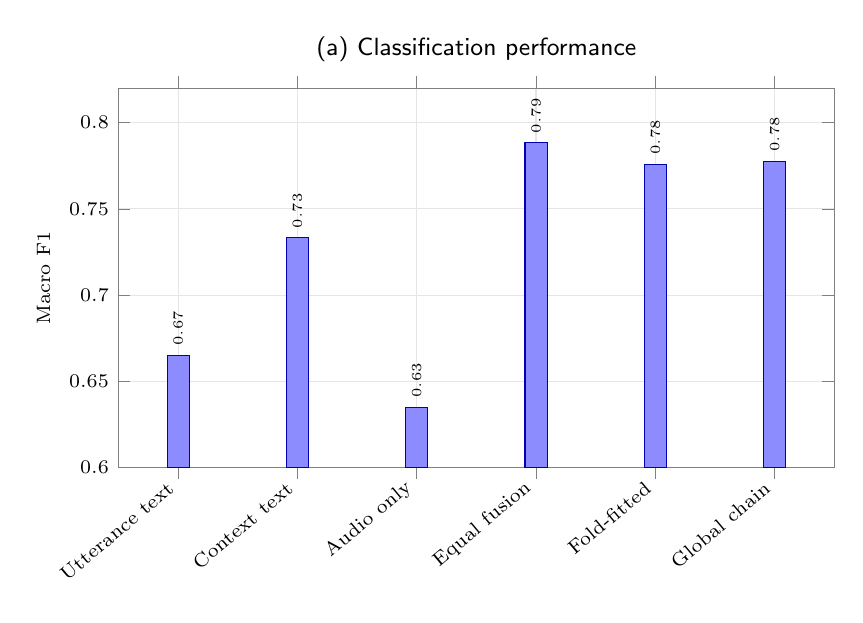
\begin{tikzpicture}
\begin{axis}[
    width=0.88\linewidth,
    height=6.4cm,
    ybar,
    bar width=8pt,
    ymin=0.60,
    ymax=0.82,
    ylabel={Macro F1},
    symbolic x coords={Utterance,Context,Audio,Equal,Fold-fit,Global},
    xtick=data,
    xticklabels={Utterance text,Context text,Audio only,Equal fusion,Fold-fitted,Global chain},
    x tick label style={rotate=40,anchor=east,font=\scriptsize},
    y tick label style={font=\scriptsize},
    ylabel style={font=\scriptsize},
    grid=major,
    grid style={draw=black!10},
    axis line style={draw=black!50},
    tick style={draw=black!50},
    nodes near coords,
    nodes near coords style={font=\tiny, rotate=90, anchor=west},
    title={(a) Classification performance},
    title style={font=\sffamily\small}
]
\addplot[fill=blue!45, draw=blue!70!black] coordinates {
    (Utterance,0.6651) (Context,0.7332) (Audio,0.6349)
    (Equal,0.7883) (Fold-fit,0.7758) (Global,0.7776)
};
\end{axis}
\end{tikzpicture}
\end{minipage}\hfill
\begin{minipage}[t]{0.40\textwidth}
\centering
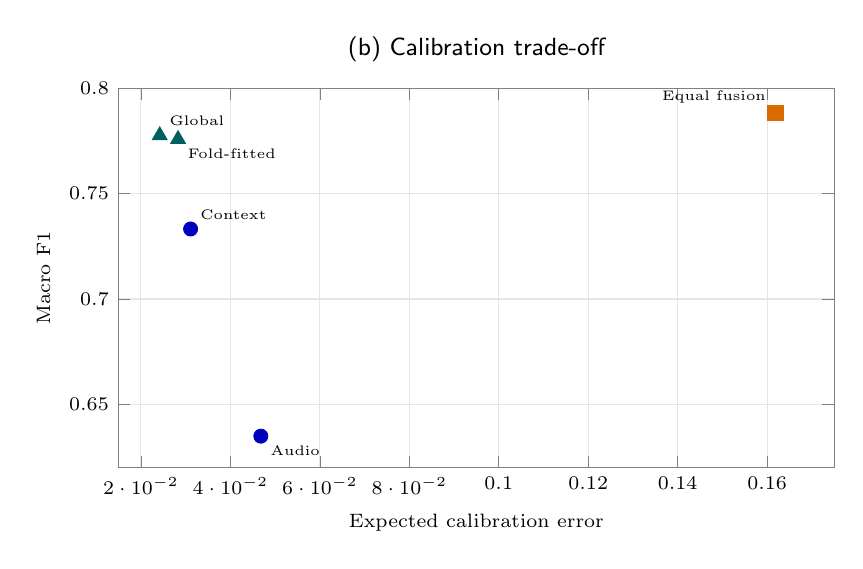
\begin{tikzpicture}
\begin{axis}[
    width=0.88\linewidth,
    height=6.4cm,
    xmin=0.015,
    xmax=0.175,
    ymin=0.62,
    ymax=0.80,
    xlabel={Expected calibration error},
    ylabel={Macro F1},
    x tick label style={font=\scriptsize},
    y tick label style={font=\scriptsize},
    xlabel style={font=\scriptsize},
    ylabel style={font=\scriptsize},
    grid=major,
    grid style={draw=black!10},
    axis line style={draw=black!50},
    tick style={draw=black!50},
    title={(b) Calibration trade-off},
    title style={font=\sffamily\small}
]
\addplot[only marks, mark=*, mark size=2.5pt, blue!75!black]
    coordinates {(0.0311,0.7332) (0.0468,0.6349)};
\addplot[only marks, mark=square*, mark size=2.8pt, orange!85!black]
    coordinates {(0.1619,0.7883)};
\addplot[only marks, mark=triangle*, mark size=3pt, teal!75!black]
    coordinates {(0.0283,0.7758) (0.0242,0.7776)};
\node[font=\tiny, anchor=south west] at (axis cs:0.0311,0.7332) {Context};
\node[font=\tiny, anchor=north west] at (axis cs:0.0468,0.6349) {Audio};
\node[font=\tiny, anchor=south east] at (axis cs:0.1619,0.7883) {Equal fusion};
\node[font=\tiny, anchor=north west] at (axis cs:0.0283,0.7758) {Fold-fitted};
\node[font=\tiny, anchor=south west] at (axis cs:0.0242,0.7776) {Global};
\end{axis}
\end{tikzpicture}
\end{minipage}

\caption{Aggregate four-class model results. Panel (a) compares macro F1, while Panel (b) shows why the highest-classification equal-weight fusion is not the preferred configuration when confidence is consumed operationally.}
\label{fig:model-results}
\end{figure}

The row-normalised confusion matrices in Figure~\ref{fig:model-confusion-matrices} expose the class-specific complementarity behind the aggregate result. Audio recognised anger more often than contextual text (78.1\% versus 69.6\% recall), whereas contextual text was substantially stronger for happiness and neutral. Equal fusion raised recall to 85.1\% for anger, 81.1\% for happiness, 66.6\% for neutral, and 85.8\% for sadness. The final global chain retained a more balanced pattern while using probabilities suitable for operational confidence.

\begin{figure}[p]
\centering
\begin{tikzpicture}
\pgfplotsset{
    dissertation confusion/.style={
        width=0.40\textwidth,
        height=0.33\textwidth,
        xmin=-0.5,
        xmax=3.5,
        ymin=-0.5,
        ymax=3.5,
        y dir=reverse,
        axis on top,
        enlargelimits=false,
        xtick={0,1,2,3},
        ytick={0,1,2,3},
        xticklabels={Ang.,Hap.,Neu.,Sad.},
        yticklabels={Anger,Happiness,Neutral,Sadness},
        tick label style={font=\scriptsize},
        label style={font=\scriptsize},
        title style={font=\sffamily\small},
        point meta min=0,
        point meta max=100,
        colormap={dissertationblue}{rgb255(0cm)=(247,251,255); rgb255(1cm)=(66,146,198)},
    },
}
\begin{groupplot}[
    group style={group size=2 by 2, horizontal sep=0.85cm, vertical sep=1.55cm},
    dissertation confusion,
]
\nextgroupplot[title={(a) Context text},ylabel={True label}]
\addplot[matrix plot*, mesh/cols=4, point meta=explicit]
    table[x=predicted,y=expected,meta=percent] {figures/data/confusion_context_text.dat};
\addplot[only marks, mark=none, point meta=explicit,
    nodes near coords={\pgfmathprintnumber[fixed,precision=0]{\pgfplotspointmeta}\%},
    nodes near coords style={font=\tiny}]
    table[x=predicted,y=expected,meta=percent] {figures/data/confusion_context_text.dat};

\nextgroupplot[title={(b) Audio only},yticklabels={}]
\addplot[matrix plot*, mesh/cols=4, point meta=explicit]
    table[x=predicted,y=expected,meta=percent] {figures/data/confusion_audio.dat};
\addplot[only marks, mark=none, point meta=explicit,
    nodes near coords={\pgfmathprintnumber[fixed,precision=0]{\pgfplotspointmeta}\%},
    nodes near coords style={font=\tiny}]
    table[x=predicted,y=expected,meta=percent] {figures/data/confusion_audio.dat};

\nextgroupplot[title={(c) Equal fusion},xlabel={Predicted label},ylabel={True label}]
\addplot[matrix plot*, mesh/cols=4, point meta=explicit]
    table[x=predicted,y=expected,meta=percent] {figures/data/confusion_equal_fusion.dat};
\addplot[only marks, mark=none, point meta=explicit,
    nodes near coords={\pgfmathprintnumber[fixed,precision=0]{\pgfplotspointmeta}\%},
    nodes near coords style={font=\tiny}]
    table[x=predicted,y=expected,meta=percent] {figures/data/confusion_equal_fusion.dat};

\nextgroupplot[title={(d) Final global chain},xlabel={Predicted label},yticklabels={}]
\addplot[matrix plot*, mesh/cols=4, point meta=explicit]
    table[x=predicted,y=expected,meta=percent] {figures/data/confusion_global_calibrated.dat};
\addplot[only marks, mark=none, point meta=explicit,
    nodes near coords={\pgfmathprintnumber[fixed,precision=0]{\pgfplotspointmeta}\%},
    nodes near coords style={font=\tiny}]
    table[x=predicted,y=expected,meta=percent] {figures/data/confusion_global_calibrated.dat};
\end{groupplot}
\end{tikzpicture}

\caption{Pooled row-normalised confusion matrices over the five held-out IEMOCAP sessions ($n=5{,}531$). Rows are true labels and columns are predicted labels; cell values are percentages of the corresponding true-label row. All panels use the same 0--100\% colour scale. The fold-fitted matrix is omitted because its class pattern is nearly identical to the final global chain.}
\label{fig:model-confusion-matrices}
\end{figure}

Figure~\ref{fig:model-reliability-curves} shows the corresponding bin-level calibration behaviour. Equal fusion lies systematically above the ideal diagonal through its populated mid-confidence region, indicating under-confidence despite its superior classification performance. Validation-fitted and global calibration move the fusion curve much closer to the diagonal. The isolated low-confidence points contain very few observations and should not be interpreted as stable local estimates.

\begin{figure}[p]
\centering
\begin{tikzpicture}
\begin{groupplot}[
    group style={group size=2 by 1, horizontal sep=1.25cm},
    width=0.47\textwidth,
    height=6.3cm,
    xmin=0.2,
    xmax=1.0,
    ymin=0.0,
    ymax=1.0,
    xtick={0.2,0.4,0.6,0.8,1.0},
    ytick={0.0,0.2,0.4,0.6,0.8,1.0},
    xlabel={Mean confidence},
    grid=major,
    grid style={draw=black!10},
    axis line style={draw=black!50},
    tick style={draw=black!50},
    tick label style={font=\scriptsize},
    label style={font=\scriptsize},
    title style={font=\sffamily\small},
    legend style={font=\tiny, draw=black!25, fill=white, cells={anchor=west}},
    unbounded coords=jump,
]
\nextgroupplot[
    title={(a) Modalities and equal fusion},
    ylabel={Empirical accuracy},
    legend pos=north west,
]
\addplot[black!55, dashed, thin, forget plot] coordinates {(0.2,0.2) (1.0,1.0)};
\addplot[blue!75!black, thick, mark=*, mark size=1.8pt]
    table[x=mean_confidence,y=accuracy] {figures/data/reliability_context_text.dat};
\addlegendentry{Context text}
\addplot[purple!75!black, thick, mark=triangle*, mark size=2.1pt]
    table[x=mean_confidence,y=accuracy] {figures/data/reliability_audio.dat};
\addlegendentry{Audio only}
\addplot[orange!90!black, thick, mark=square*, mark size=1.9pt]
    table[x=mean_confidence,y=accuracy] {figures/data/reliability_equal_fusion.dat};
\addlegendentry{Equal fusion}

\nextgroupplot[
    title={(b) Fusion calibration},
    legend pos=north west,
]
\addplot[black!55, dashed, thin, forget plot] coordinates {(0.2,0.2) (1.0,1.0)};
\addplot[orange!90!black, thick, mark=square*, mark size=1.9pt]
    table[x=mean_confidence,y=accuracy] {figures/data/reliability_equal_fusion.dat};
\addlegendentry{Equal fusion}
\addplot[teal!75!black, thick, mark=triangle*, mark size=2.1pt]
    table[x=mean_confidence,y=accuracy] {figures/data/reliability_validation_fitted.dat};
\addlegendentry{Fold-fitted}
\addplot[blue!75!black, thick, mark=diamond*, mark size=2.2pt]
    table[x=mean_confidence,y=accuracy] {figures/data/reliability_global_calibrated.dat};
\addlegendentry{Global chain}
\end{groupplot}
\end{tikzpicture}

\caption{Reliability curves from pooled held-out predictions. Each point represents a non-empty equal-width bin of maximum class probability; the dashed diagonal denotes perfect calibration. Panel (a) compares the unimodal systems with predeclared equal fusion, and Panel (b) shows the effect of validation-derived fusion calibration. ECE values in Table~\ref{tab:calibration-tradeoff} use the prespecified 15-bin calculation, while the curves use ten bins for legibility.}
\label{fig:model-reliability-curves}
\end{figure}
\clearpage

The final global chain also obtained negative log-likelihood 0.6075 and multiclass Brier score 0.3280. It is the configuration stored for full-data packaging because it provides the single parameter set required by one final text model and one final audio model. However, its pooled calibration fitting uses all out-of-fold validation rows and is an operational configuration analysis, not a new independent confirmatory comparison. The equal-weight result remains the classification headline.

\subsection{Answer to RQ2}
\label{subsec:rq2-answer}

RQ2 is also answered positively within IEMOCAP. Equal-weight late fusion improved macro F1 by 0.0551 over contextual text and by 0.1534 over audio alone, showing complementary information in the textual and acoustic branches. The paired interval against contextual text excluded zero.

The answer includes a material trade-off: the strongest classifier was poorly calibrated, whereas validation-fitted and global calibration configurations sacrificed approximately one percentage point of macro F1 while reducing ECE substantially. AffectLab therefore uses the global validation-derived chain for operational confidence and retains conservative presentation rules. Calibration under IEMOCAP does not guarantee calibration after distribution shift \,\cite{ovadia2019shift}.

\section{Application Verification and Readiness}
\label{sec:engineering-evaluation}

Table~\ref{tab:requirements-traceability} provides a compact trace from the requirements in Chapter~\ref{chap:proposed-system-architecture} to their implementation and verification evidence. Requirements are grouped only where they share the same implementation boundary, verification method, outcome, and principal limitation. Here, ``passed'' means conformance under the cited developer-led checks, not universal validation beyond the tested configuration.

\begin{table}[p]
\centering
\caption{Compact requirement-to-evidence traceability matrix.}
\label{tab:requirements-traceability}
\scriptsize
\setlength{\tabcolsep}{3pt}
\renewcommand{\arraystretch}{0.96}
\begin{tabularx}{\textwidth}{|>{\raggedright\arraybackslash}p{0.16\textwidth}|>{\raggedright\arraybackslash}p{0.19\textwidth}|>{\raggedright\arraybackslash}p{0.24\textwidth}|>{\raggedright\arraybackslash}p{0.09\textwidth}|X|}
\hline
\textbf{Requirement IDs} & \textbf{Implementation location} & \textbf{Verification method} & \textbf{Outcome} & \textbf{Principal limitation} \\ \hline
FR1, FR26; NFR5, NFR13 & Authentication, persistence, isolation, and deletion (Sections~\ref{subsec:backend-authentication}, \ref{subsec:backend-session-persistence}, and \ref{sec:security-privacy-data-protection}) & API, security, ownership, stale-write, deletion, and MongoDB recovery tests & Passed & No independent penetration test or deployed backup exercise \\ \hline
FR2, FR3, FR25; NFR3 & Onboarding, preferences, takeaways, and action cards (Sections~\ref{subsec:frontend-navigation} and \ref{subsec:takeaways-action-cards}) & API and browser onboarding, preference, reflection, and recovery journeys & Passed & No independent usability assessment of these controls \\ \hline
FR4--FR8, FR15, FR19 & Preparation, scenario configuration, lifecycle, and dialogue policies (Sections~\ref{subsec:frontend-preparation}, \ref{subsec:scenario-representation}, and \ref{subsec:dialogue-transitions}) & Policy/unit, API, desktop/mobile browser, authored-trajectory, and smoke tests & Passed & Three standard scenarios and controlled inputs \\ \hline
FR9, FR11--FR13; NFR2, NFR4 & Voice, causal-context inference, fusion, and fallback paths (Sections~\ref{sec:emotion-recognition-pipeline}, \ref{subsec:frontend-voice}, and \ref{subsec:audio-conversation-data}) & Context, multimodal, transcription, transient-audio, missing-service, and browser tests & Passed in tested configuration & Limited live-device, provider, and private-model execution \\ \hline
FR10; NFR1 & Crisis interruption and safety precedence (Section~\ref{subsec:safety-precedence}) & Crisis paraphrase, false-positive, precedence, API, and conversation tests & Passed & A bounded lexical detector cannot cover every expression \\ \hline
FR29 & Cognitive heuristics and strategy selection (Subsection~\ref{subsec:cognitive-support-routing}) & Authored unit and service cases for pattern, intent, clause extraction, pushback, strategy, and safety precedence & Passed as rule conformance only & No construct, predictive, clinical, comparative-helpfulness, or harm evaluation \\ \hline
FR14; NFR14 & Bounded affect pacing and uncertainty presentation (Sections~\ref{subsec:affect-pacing} and \ref{subsec:frontend-affect-presentation}) & Seven authored policy cases plus preference, disagreement, failure, and replay tests & Passed & Controlled probabilities; no evidence of user benefit \\ \hline
FR16--FR18, FR20--FR21; NFR6, NFR8 & Evidence, response realisation, fallback, and feedback (Sections~\ref{subsec:communication-evidence}, \ref{subsec:response-realisation}, and \ref{subsec:evidence-feedback}) & Determinism, evidence-linking, constrained-generation, fallback, feedback, and concurrency tests & Passed & Designed cases do not exhaust language variation \\ \hline
FR22--FR24 & Replay, retry, branching, and comparison (Sections~\ref{subsec:conversation-replay} and \ref{subsec:rewind-branching}) & Backend, browser, stale-state, restart-persistence, and full-stack smoke tests & Passed & Synthetic histories rather than natural long-term use \\ \hline
FR27--FR28; NFR7 & Consent, study progress, pseudonymous export, and versioning (Section~\ref{sec:research-workflow-implementation} and Subsection~\ref{subsec:reproducibility-provenance}) & Protocol, eligibility, withdrawal, export-exclusion, dataset-freeze, provenance, and smoke tests & Passed & No independent privacy or reproduction audit \\ \hline
NFR9 & Health, bounded failures, recovery, and local responsiveness (Subsections~\ref{subsec:health-failure-handling} and \ref{subsec:performance-testing}) & Recovery journeys, health checks, full-stack restart, and performance regression artefact & Passed locally & No networked concurrent-load or provider-latency test \\ \hline
NFR10 & Accessible and responsive interface (Subsections~\ref{subsec:frontend-navigation} and \ref{subsec:frontend-testing}) & axe-core scans, keyboard assertions, and desktop/mobile browser runs & Passed tested views & No evaluation with users with disabilities \\ \hline
NFR11--NFR12 & Modular and testable architecture (Sections~\ref{subsec:backend-service-architecture} and \ref{sec:implementation-verification}) & Interface inspection, provider substitution, and automated suites across component boundaries & Shown & Maintainability was not measured longitudinally \\ \hline
\end{tabularx}
\end{table}

\subsection{Deterministic Dialogue Cases}
\label{subsec:dialogue-case-results}

The versioned engineering evaluator contains five authored trajectories for enhanced workload, boundary, and relationship practice. Each specifies the user turns and expected sequence of controller stages. All five enhanced trajectories matched their expected sequence, as shown in Table~\ref{tab:dialogue-case-results}. The fixed controller is included only to expose the change in policy granularity; it stops according to its own earlier completion conditions and is not treated as a human-performance baseline.

\begin{table}[htbp]
\centering
\caption{Authored enhanced-dialogue trajectory results.}
\label{tab:dialogue-case-results}
\footnotesize
\begin{tabularx}{\textwidth}{|>{\raggedright\arraybackslash}p{0.18\textwidth}|X|>{\raggedright\arraybackslash}p{0.20\textwidth}|}
\hline
\textbf{Case} & \textbf{Expected and observed enhanced stages} & \textbf{Final state} \\ \hline
Workload agreement & constraints $\rightarrow$ agree $\rightarrow$ resolved & Completed: success \\ \hline
Workload non-confirmation & constraints $\rightarrow$ agree $\rightarrow$ agree & Active; no false agreement \\ \hline
Boundary maintained & pressure $\rightarrow$ resolved & Completed: success \\ \hline
Relationship next step & perspective $\rightarrow$ agree $\rightarrow$ resolved & Completed: success \\ \hline
Relationship unresolved & perspective $\rightarrow$ unresolved & Completed: unresolved \\ \hline
\end{tabularx}
\end{table}

These cases show that the enhanced controller requires intermediate evidence rather than completing as soon as one generic success phrase is detected. They do not show that its dialogue is more persuasive, realistic, or educational for a participant. Those properties require human evaluation.

\subsection{Cognitive-Heuristic and Support-Routing Cases}
\label{subsec:cognitive-routing-results}

The cognitive and strategy tests are small, implementation-authored examples rather than a labelled evaluation dataset. Table~\ref{tab:cognitive-routing-cases} states exactly what they establish. The combined sentence deliberately activates several rules at once; the test verifies that the documented precedence and extraction code are stable, not that a human assessor would assign the same psychological labels.

\begin{table}[htbp]
\centering
\caption{Implemented cognitive-heuristic and support-routing checks.}
\label{tab:cognitive-routing-cases}
\footnotesize
\begin{tabularx}{\textwidth}{|>{\raggedright\arraybackslash}p{0.28\textwidth}|>{\raggedright\arraybackslash}p{0.31\textwidth}|X|}
\hline
\textbf{Authored input or condition} & \textbf{Verified implementation result} & \textbf{What the check does not establish} \\ \hline
``They will definitely think I am a failure because I missed one deadline. What should I do?'' & A cognitive-pattern rule matches; practical-help wins the intent precedence; the clause after \emph{because} is copied as possible context & That the speaker has a cognitive distortion, that the copied clause is the true cause, or that practical advice is wanted \\ \hline
``But that won't work. This is pointless.'' & The explicit pushback vocabulary produces a resistance value above the selector threshold & Psychological resistance, its degree, persistence, or cause \\ \hline
``How do I handle this?'' with the default lexical affect state & Practical-help routing makes practical suggestion the highest-scoring strategy & That the suggestion is helpful, well timed, or superior to clarification or reflection \\ \hline
Crisis flag true with high arousal & Safety escalation wins over all ordinary strategy scores & Sensitivity or specificity of crisis detection, or adequacy of the safety response \\ \hline
Two authored emotional-support messages & The analyser, selector, and offline template compose a non-generic emotion-specific response & Accuracy of the affect or intent label, user preference, therapeutic value, or absence of harm \\ \hline
\end{tabularx}
\end{table}

These checks cover selected positive paths and one precedence condition. They do not systematically test all ten pattern families, all combinations and tie cases, negated and quoted pattern language, malformed causal clauses, demographic or dialectal variation, or user correction of a wrong inference. The browser suite verifies rendering of deterministic decision data but does not independently validate the semantics of the labels. Consequently, the appropriate result is ``conforms to the tested rules'', not an accuracy percentage. The subsystem did not contribute an outcome measure to the pilot, and no claim is made that its labels or selected strategies improved the participant experience.

\subsection{Evidence Extraction and Affect-Pacing Cases}
\label{subsec:policy-case-results}

Twelve human-authored feature judgements were compared with the deterministic extractor. The fixture produced five true positives, four true negatives, one false positive, and two false negatives. Reported speech containing ``I need'' was incorrectly attributed to the current speaker; an indirect refusal and the synonym ``shift'' were missed. With only twelve designed cases, these counts are diagnostic examples rather than a held-out accuracy estimate. Importantly, the errors expose the intended limitation of a bounded lexical policy and justify replaying the complete source utterance.

Seven controlled affect cases exercised matching confident estimates, modality disagreement, low confidence, missing audio, an unavailable model, disabled adaptation, and an explicit user choice. All seven produced the declared action. Matching high-confidence sadness allowed a brief acknowledgement; disagreement and low confidence offered a pacing choice; unavailable evidence and disabled adaptation preserved the baseline; and the explicit gentler preference took precedence. Separate tests verify that safety, completion, ineligible sessions, and required study tasks override adaptation.

The deterministic evaluator recorded median in-process service latency of approximately 0.64~ms and a lower-order-statistic 95th-percentile value of approximately 3.46~ms across 19 calls. These figures exclude HTTP, MongoDB, provider generation, and trained inference and are not a load test or production latency claim.

\subsection{Automated and Full-Stack Verification Results}
\label{subsec:automated-system-results}

The default backend run performed for the completed implementation reported 240 passing tests and 13 skipped tests. The skipped group contains opt-in checks requiring an external environment, including real MongoDB or private model conditions; it is not counted as a passing result. The frontend production TypeScript build, Vite build, ESLint check, and backend Ruff check completed successfully. These runs verify the current code paths but do not replace the versioned evidence artefacts.

The saved full-stack smoke manifest reports two passing browser journeys against a compiled frontend, actual FastAPI process, and disposable MongoDB 8.0.1 database. The journeys included account access, pre-consent exclusion, enrolment, a required task and questionnaire, researcher export, enhanced dialogue, network-failure recovery, replay, branching, comparison, and action-card persistence. The backend was stopped and relaunched twice while MongoDB remained active, and persisted state was verified after each relevant restart. The recorded total run time was 95.72 seconds; this is demonstration timing, not a capacity benchmark.

Together, these complementary checks support the requirement outcomes summarised in Table~\ref{tab:requirements-traceability}; their principal scope limitations are reported in the same table.

\subsection{Performance and Responsive-Interface Checks}
\label{subsec:performance-results}

A reproducible local benchmark exercised the HTTP boundary of the deterministic core using FastAPI's in-process transport and the memory repository. It included routing, bearer-token authentication, request validation, application services, and response serialisation. After warm-up, the benchmark collected 200 samples for read-only endpoints and 100 samples for each state-changing workflow operation. Table~\ref{tab:performance-results} reports the results from the recorded Windows~11 and Python~3.14.3 run.

\begin{table}[htbp]
\centering
\caption{Local single-client application latency results.}
\label{tab:performance-results}
\begin{tabular}{|l|r|r|r|}
\hline
\textbf{Operation} & \textbf{Samples} & \textbf{Median (ms)} & \textbf{95th percentile (ms)} \\ \hline
Liveness endpoint & 200 & 1.332 & 1.866 \\ \hline
Authenticated scenario catalogue & 200 & 2.942 & 3.922 \\ \hline
Session creation & 100 & 2.988 & 3.961 \\ \hline
Role-play start & 100 & 3.396 & 4.437 \\ \hline
Deterministic conversation turn & 100 & 4.659 & 5.836 \\ \hline
\end{tabular}
\end{table}

The benchmark is a fast regression check for local application overhead, not a production-capacity test. It excludes network latency, MongoDB, external generation and transcription providers, trained multimodal inference, and concurrent clients. Those variables depend on the deployed environment and require a separate staged load test. Within its declared scope, however, the result shows that the locally controlled text-first path adds only a few milliseconds per request and that optional services are not on the critical path when deterministic fallbacks are used. All five measurements passed their predeclared 95th-percentile regression budgets. The JSON evidence artefact records the environment, sample counts, budgets, source hashes, individual scope exclusions, and summary statistics.

Perceived responsiveness also depends on the browser rather than API latency alone. The frontend therefore runs as a compiled production build in both desktop Chromium and a Pixel~7 mobile profile. The browser suite verifies responsive layouts, keyboard interaction, focus behaviour, live status messages, preservation of unsent input after failure, and immediate recovery controls. These checks support the claim that the interface is responsive across the tested viewports; they do not replace field measurements of Core Web Vitals on the eventual hosting infrastructure.

\subsection{Answer to RQ3}
\label{subsec:rq3-answer}

RQ3 asks how uncertain multimodal predictions can be integrated while keeping behaviour explainable, controllable, safe, and failure-tolerant. The implementation and engineering evidence provide a constructive answer: the classifier output is validated and stored as evidence; a deterministic policy maps confidence, agreement, availability, eligibility, and user preference to a small action set; the dialogue controller remains authoritative; and each action and fallback reason is persisted for replay.

The authored cases and automated tests show that low confidence and disagreement produce a user choice, missing inference preserves the baseline, explicit preference takes precedence, and safety bypasses model adaptation. Version-bound requests and optimistic persistence attach a prediction to its exact exchange. This establishes specified system behaviour under the tested conditions. It does not establish that the emotion label itself is correct for a real participant or that pacing improves their outcome.

\subsection{Answer to RQ4: Integrated Application Quality}
\label{subsec:rq4-status}

RQ4 is answered through the combined evidence traced in Table~\ref{tab:requirements-traceability}. The automated, browser, full-stack, recovery, and authored-policy checks passed in the tested configuration, while the locally controlled text-first operations remained below 7~ms at the 95th percentile. These results support readiness for a controlled production deployment with that configuration.

This conclusion is deliberately environment-specific. It does not claim internet-scale capacity or guarantee the latency of MongoDB, trained inference, or external providers. A public deployment should establish its own service-level objectives and repeat concurrent-load, network, backup, security, and observability checks in staging.

\subsection{Supplementary User-Pilot Results}
\label{subsec:participant-results}

\paragraph{Scope of the pilot result.} The pilot did not evaluate multimodal affect adaptation. Every required task was ineligible for multimodal inference and affect-aware pacing, so participants completed the baseline text-based rehearsal with deterministic dialogue and feedback. Accordingly, the ratings below describe that baseline experience only: they cannot establish whether emotion-aware adaptation is acceptable, useful, or beneficial. Evidence concerning the classifier and the implemented adaptation policy instead comes from the IEMOCAP experiments in Section~\ref{sec:multimodal-results} and the authored, automated, and full-stack tests reported above; those tests establish benchmark performance and policy conformance within their stated scopes, not human benefit.

Within that boundary, the supplementary single-arm pilot examined completion of the baseline rehearsal workflow and collected brief usability ratings. The analysis uses the AffectLab feasibility protocol v1.1 export, with the first attempt at each required intermediate-difficulty scenario selected for the protocol outcomes. The analytic export includes 15 participants and 46 rehearsal sessions, of which 42 were first required attempts and four were additional or retry sessions. Of the required attempts, 39 reached task completion (14 workload, 13 boundary, and 12 relationship). Twelve participants completed all three required scenarios and submitted the corresponding post-rehearsal questionnaires, giving a protocol-completion rate of 80.0\% (12/15; two-sided 95\% Wilson interval 54.8\%--93.0\%). The point estimate met the protocol's 80\% feasibility target, although the interval remained wide at this sample size.

Table~\ref{tab:pilot-questionnaire-results} summarises the available study-specific ratings. Feedback usefulness and scenario realism for the non-adaptive required tasks had means of 5.33 and 4.85, respectively, on seven-point scales. These scores concern the deterministic feedback and scenario experience, not multimodal inference or affect-aware pacing. Among 38 observations with both confidence ratings available, representing 14 participants, the mean within-task confidence change was +0.97 points (median +1; participant-cluster bootstrap 95\% interval +0.67 to +1.26). The mean paired changes were +0.85 for workload ($n=13$), +0.85 for boundary ($n=13$), and +1.25 for relationship ($n=12$). These within-task differences reflect immediate self-report, not independently verified communication improvement or an effect attributable to the application.

\begin{table}[htbp]
\centering
\caption{Supplementary pilot questionnaire results from available first required attempts. Ratings use seven-point scales; paired change is post-confidence minus pre-confidence.}
\label{tab:pilot-questionnaire-results}
\footnotesize
\begin{tabular}{|l|r|r|r|r|c|}
\hline
\textbf{Measure} & \textbf{$n$} & \textbf{Mean} & \textbf{SD} & \textbf{Median} & \textbf{Q1--Q3} \\ \hline
Pre-rehearsal confidence & 40 & 3.80 & 1.04 & 4.0 & 3.0--4.0 \\ \hline
Pre-rehearsal anxiety & 40 & 4.58 & 1.28 & 5.0 & 4.0--5.25 \\ \hline
Post-rehearsal confidence & 40 & 4.75 & 1.37 & 4.5 & 4.0--6.0 \\ \hline
Scenario realism & 40 & 4.85 & 0.98 & 5.0 & 4.0--5.25 \\ \hline
Feedback usefulness & 40 & 5.33 & 0.92 & 5.0 & 5.0--6.0 \\ \hline
Paired confidence change & 38 & +0.97 & 0.97 & +1.0 & 0.25--1.75 \\ \hline
\end{tabular}
\end{table}

The deterministic feedback also produced scenario-specific lexical indicators on the 39 completed required tasks. Mean scores included 42.3\% for clear requests in workload rehearsal ($n=14$), 59.0\% for clear refusal or maintained boundaries ($n=13$), and 44.4\% for use of an I-statement in relationship rehearsal ($n=12$). The configured absence-of-blame indicators reached 100\% in workload and relationship tasks, and the no-repeated-apology indicator reached 100\% in boundary tasks. These are averages of rule-defined scores rather than percentages of participants demonstrating validated skills; the indicators were not independently annotated or established as measures of real-world communication ability. They provide limited behavioural context to the stronger engineering evidence for the feedback implementation.

Two required attempts lacked a post-questionnaire, and only 38 of the 42 required attempts contained a valid pair of confidence ratings. Consequently, questionnaire summaries use available observations and report their denominators rather than imputing responses. The pilot offers preliminary evidence of workflow uptake and perceived usefulness, but the small convenience sample and uncontrolled design preclude causal, clinical, or generalisable effectiveness claims. It is therefore treated as a supplement to the model and system-verification results, not as the principal basis for deployment readiness.

\section{Threats to Validity and Limitations}
\label{sec:evaluation-limitations}

\subsection{Model and Statistical Validity}
\label{subsec:model-validity-threats}

The five test folds cover all IEMOCAP sessions, but the corpus contains only ten actors. Fold results are therefore dependent on a small set of speakers, acted or improvised tasks, recording conditions, and annotation practices. The dialogue bootstrap reflects the 151 observed conversations but cannot compensate for missing demographic, cultural, linguistic, and environmental diversity. Only one primary training seed was used after the pipeline check, so optimisation variance is not fully characterised.

Repeated GPU execution can produce small numerical variation. The reported paired comparisons use the latest internally consistent private prediction files, each checked against its neighbouring metrics record. This preserves internal pairing but illustrates why commit, configuration, and file hashes are necessary. The final full-data packages cannot be evaluated on their training rows, and their file-level provenance remains incomplete until the private directories are downloaded and hashed beside the application.

ECE is bin-dependent, and calibration can deteriorate under shift. The global deployment chain is fitted from pooled validation roles across the corpus; it is useful for choosing one full-data configuration but is not an independent external calibration study. The 0.55 and 0.75 presentation bands are operational thresholds rather than validated psychological boundaries.

\subsection{External and Construct Validity}
\label{subsec:external-validity-threats}

IEMOCAP labels describe annotated expressive categories, not direct measurements of internal emotion. Mapping excitement to happiness and fear to exploratory anxiety further simplifies the constructs. Model performance must not be interpreted as diagnosis, emotional truth, or equitable performance across accents, languages, devices, ages, disabilities, or cultures.

The role-play features are likewise operational constructs. A phrase detector can identify authored patterns such as a clear refusal or practical request, but it does not measure general communication ability or transfer to a real conversation. The diagnostic fixture already demonstrates missed synonyms, indirect language, and reported-speech error. Deterministic feedback is more auditable than an unconstrained judgement, but it remains limited by these definitions.

The rule-based cognitive fields have an even narrower evidential basis. Familiar labels such as cognitive distortion, intent, cause, readiness, and resistance may suggest assessment of an internal state, but the implementation observes only the current message and assigns fixed values when short patterns occur. No clinician, validated questionnaire, independent annotator, held-out corpus, or participant self-report was used as a reference standard. The tests reported in Subsection~\ref{subsec:cognitive-routing-results} establish software conformance, not accuracy, construct validity, or clinical validity. Because the pilot neither isolated this subsystem nor measured its helpfulness or harms, the selected support strategy cannot be claimed to be optimal or beneficial. False and overly authoritative labels remain a risk, especially for negation, quotation, indirect language, cultural variation, and messages containing several possible requests.

The engineering evaluation largely uses deterministic templates and test accounts. It does not evaluate live provider variability, private-model latency under concurrent participant use, real microphone noise, or long-duration deployment. The successful smoke journey establishes integration and restart persistence only for its tested path.

\subsection{Supplementary User-Evidence Limitations}
\label{subsec:participant-validity-threats}

The supplementary pilot was single-arm and included only 15 participants in the analytic export, limiting precision and generalisability. More fundamentally for the present dissertation, required tasks bypassed multimodal inference and affect-aware pacing. The pilot therefore provides no direct user evidence about whether the emotion-aware adaptation was acceptable, accurate, intrusive, helpful, or harmful; its realism and usefulness scores apply only to the baseline rehearsal and deterministic feedback that participants encountered. The wide confidence interval around protocol completion illustrates additional uncertainty. Missing ratings, incomplete rehearsals, fixed scenario order, repeated exposure, self-selection, and demand characteristics may influence the descriptive findings. The study-specific ratings are not validated clinical scales, and the deterministic lexical scores were not validated against independent assessments of communication quality. Without a control condition or follow-up assessment, the observed immediate confidence change cannot establish causation, sustained skill development, or transfer to real conversations. These limitations are why the pilot contributes contextual usability evidence rather than the principal validation of the application or evidence for affect-aware adaptation.

\section{Chapter Summary}
\label{sec:evaluation-summary}

The evaluation provides completed answers to the two machine-learning questions. Three-turn causal context improved the four-class text model from 0.6651 to 0.7332 macro F1, with a paired dialogue-bootstrap interval excluding zero. Equal-weight text--audio fusion further improved macro F1 to 0.7883, demonstrating complementary benchmark information. However, its ECE of 0.1619 exposed a classification--calibration trade-off. Validation-derived calibration reduced ECE substantially at a modest classification cost, motivating the global text-dominant configuration used for final packaging.

The application evaluation answers RQ3 and RQ4 at the level of specified, reproducible system behaviour. All five authored enhanced dialogue trajectories and all seven affect-pacing decisions matched expectations. Diagnostic evidence cases exposed one false positive and two false negatives rather than concealing lexical limitations. A 240-test backend run, production frontend checks, desktop/mobile browser and accessibility tests, two full-stack journeys, persistence across backend restarts, and local HTTP timings verify complementary functional and non-functional boundaries. The deterministic conversation path recorded a median of 4.659~ms and a 95th percentile of 5.836~ms in the scoped local benchmark.

The small pilot remains supporting evidence for the non-adaptive workflow: 12 of 15 participants completed the three required rehearsals and questionnaires, while mean scenario-realism and feedback-usefulness ratings were 4.85 and 5.33 out of seven. Because those required rehearsals bypassed multimodal inference and affect-aware pacing, these observations say nothing about the acceptability or benefit of emotion-aware adaptation. The evaluation therefore rests principally on the separate model benchmark and the authored, automated, browser, persistence, recovery, full-stack, accessibility, and performance tests. Overall, AffectLab is a fully implemented communication-practice system whose model behaviour, core policies, interfaces, persistence, accessibility, recovery, and local responsiveness have been tested extensively by the developer and through automation, with human evaluation of adaptation and deployment-scale performance appropriately reserved for future controlled and staging studies.

\chapter{Conclusions and Future Work}
\label{chap6}

\section{Conclusions for the Research Questions}
\label{sec:conclusion-research-questions}

This dissertation asked whether conversational context and speech provide useful affective evidence, how such evidence can be used without giving a classifier authority over a role-play, and whether the resulting application meets its declared engineering requirements. The evaluation in Chapter~\ref{chap5} supports the following bounded answers.

\paragraph{RQ1: conversational context.}
\label{subsec:conclusion-rq1}
Preceding dialogue turns improved text-based emotion classification under the declared four-class, speaker-independent IEMOCAP protocol. The paired dialogue-level comparison consistently favoured the contextual model, so the improvement cannot be attributed to different speakers, label sets, or optimisation settings. This is evidence that causal conversational context helps classify annotated expression in this benchmark; it is not evidence that the model recovers a person's private emotional state or that the gain will transfer unchanged to spontaneous AffectLab conversations. The exploratory six-class result points in the same aggregate direction but is too sparse to support an anxiety-recognition claim.

\paragraph{RQ2: multimodal complementarity and calibration.}
\label{subsec:conclusion-rq2}
Acoustic information was complementary to contextual text even though audio was the weaker individual modality. Predeclared equal-weight fusion improved the principal classification measures over either unimodal model, with the paired bootstrap comparison favouring fusion. However, this configuration was substantially less calibrated than contextual text. Validation-fitted fusion recovered strong calibration while retaining most of the classification gain. The answer is therefore conditional: multimodal fusion improved benchmark classification, but the configuration that maximised classification was not the configuration with the most trustworthy probabilities. Classification and calibration must be selected and reported separately when confidence affects adaptive behaviour.

\paragraph{RQ3: bounded use of affective evidence.}
\label{subsec:conclusion-rq3}
Uncertain predictions can be integrated responsibly by restricting what they are allowed to change. AffectLab records the prediction and its provenance, checks confidence, modality agreement, availability, eligibility, and user preference, and maps the result to a small set of reversible pacing actions. Deterministic scenario controllers remain authoritative for progression and outcomes; observable language evidence determines feedback; explicit safety handling takes precedence; and inference failure preserves the baseline workflow. Authored policy cases and integrated journeys conformed to these rules. This establishes explainable and failure-tolerant policy behaviour under tested conditions, not that an affect estimate is correct for a particular user or that adaptation improves rehearsal outcomes.

\paragraph{RQ4: integrated application quality.}
\label{subsec:conclusion-rq4}
The completed application satisfied its scoped functional and non-functional requirements for the tested offline deterministic core. Backend, production-frontend, browser, automated-accessibility, persistence, recovery, and full-stack checks supported the declared behaviours, while the local regression benchmark met every response-time budget. These layers establish an implementation-complete, deployment-oriented system rather than deployment readiness. The performance run excluded real network transit, production persistence, trained inference, external providers, concurrency, and adversarial traffic. A controlled deployment therefore remains conditional on target-environment performance, security, observability, backup recovery, and incident-response validation.

\section{Contributions and Material Limitations}
\label{sec:conclusion-contributions}

The work makes three connected contributions. Empirically, it provides a controlled speaker-independent comparison of utterance-only and contextual text classification, followed by a text--audio study that treats calibration as distinct from classification. Architecturally, it demonstrates a hybrid role-play system in which probabilistic models and optional generation influence presentation without controlling dialogue outcomes, assessment, or safety. Methodologically, it separates benchmark evidence, deterministic policy conformance, application verification, local performance, and supplementary user feedback so that one evidence type is not used to support a stronger claim than it can bear. Versioned policies, provenance, evidence-grounded feedback, fallbacks, and replayable state make the implemented decisions inspectable.

These contributions are bounded by the available data and evaluation. IEMOCAP contains ten actors in acted or improvised English dialogue and does not provide external, cultural, device, or deployment validation. A single primary training seed leaves optimisation variability incompletely characterised, while full-data packages and the operational fusion summary have no independent held-out estimate. Emotion categories and confidence thresholds are operational signals rather than psychological measurements. The three scenario policies and lexical feedback rules cover limited forms of communication, and the separately implemented cognitive support-routing fields are unvalidated heuristics, not measures of cognition, intention, readiness, resistance, or clinical state.

The engineering tests used controlled inputs and synthetic accounts, and automated accessibility checks do not replace evaluation with assistive-technology users. Most importantly, the small, uncontrolled pilot exercised the deterministic baseline rather than multimodal inference or affect-aware pacing. It can inform workflow refinement but cannot establish adaptation benefit, sustained learning, transfer, or absence of harm. AffectLab is consequently a communication-practice research application, not a diagnostic, clinical, crisis, or therapeutic system.

\section{Prioritised Future Work}
\label{sec:conclusion-future-work}

The immediate priority is deployment-specific validation of the existing system. A staging study should exercise the packaged models, external providers, intended database, real network path, and representative concurrency. Declared service objectives, load and soak tests, provider and database failures, backup restoration, security review, monitoring, and incident exercises should establish latency, capacity, recovery, and operational risk before any production-readiness claim.

The next priority is to strengthen the evidence behind both inference and interaction. Cross-corpus and target-context evaluation should examine calibration under language, microphone, noise, transcription, and demographic variation, using repeated seeds and prospective held-out data. Independent human annotation should assess the validity and error patterns of feedback rules; psychologically suggestive support-routing labels should be removed, renamed as observable behaviour, or subjected to appropriate expert and ethics-led validation. A preregistered comparison of the baseline and bounded affect-aware policy should then measure helpfulness, intrusiveness, task outcomes, and user preference without treating engagement as benefit.

Longer-term work should use participatory accessibility testing, multilingual and cultural adaptation, and longitudinal studies of retention and transfer. These studies should preserve opt-in controls, data minimisation, transparent uncertainty, and a useful non-adaptive baseline. Model, prompt, scenario, threshold, and safety-resource changes should remain versioned and governed as the evidence base develops.

\section{Final Conclusion}
\label{sec:final-conclusion}

This dissertation shows that contextual and acoustic affective evidence can improve benchmark classification and can be connected to role-play without making emotion recognition authoritative. AffectLab combines bounded adaptation with deterministic progression, evidence-grounded feedback, safety precedence, user control, and auditable fallbacks. Its evaluation establishes the implemented system and policies within clearly defined test conditions, while leaving claims about emotional truth, human benefit, and production readiness to future evidence. Within those limits, the work provides a reproducible foundation for studying emotion-aware communication rehearsal while preserving uncertainty and user agency.



\bibliography{myBib}
\bibliographystyle{alpha}
\addcontentsline{toc}{chapter}{Bibliography}


\appendix
\chapter{Generative AI Tools Usage}
\label{genAIUsage}

Generative AI tools were used as supplementary resources during the development and documentation of this thesis. Their use was limited to supporting literature exploration, improving the clarity of academic writing, assisting with LaTeX formatting, and providing guidance during technical problem-solving. All generated suggestions were reviewed before being incorporated into the thesis.

An overview of the generative AI tools used is presented in Table \ref{tab:genAIOverview}.

\rowcolors{2}{gray!15}{white}
\begin{table}[h!]
    \centering
    \begin{tabularx}{\textwidth}{|l|X|X|X|}
        \hline
        \rowcolor{blue!20}
        AI Tool & Use Case & Used in & Remarks \\ \hline

        \multirow{4}{*}{\shortstack[l]{ChatGPT\\5.6 Sol /\\6 Astra}}
        & Literature exploration and identification of relevant scientific publications
        & Chapter 2
        & Suggested references were independently verified \\ \cline{2-4}

        & Improvement of academic phrasing, grammar, and text clarity
        & Chapters 1--5
        & Suggestions were reviewed and adapted \\ \cline{2-4}

        & Assistance with LaTeX syntax, formatting, and document structure
        & Entire thesis
        & Formatting suggestions were manually checked \\ \cline{2-4}

        & Technical guidance and debugging suggestions
        & Implementation chapters
        & Suggestions were evaluated and tested before use \\ \hline

    \end{tabularx}
    \caption{Overview of generative AI usage}
    \label{tab:genAIOverview}
\end{table}

\section{ChatGPT Details}
\label{sectionChatGPT}

ChatGPT (versions 5.6 Sol and 6 Astra, developed by OpenAI) was used as a supplementary assistant throughout selected stages of the thesis. Its contributions are described below.

\subsection{Literature Exploration}

\textbf{Purpose:}
To support the identification of relevant scientific publications and research directions related to the topics investigated in this thesis.

\textbf{Method:}
ChatGPT was prompted to suggest academic publications, relevant research topics, and potential directions for organizing the state-of-the-art review in Chapter 2.

\textbf{Verification:}
Suggested publications were checked against academic sources to verify their existence, relevance, and bibliographic information. The original publications were consulted before being referenced.

\textbf{Implementation:}
The verified references and research directions were used as supporting resources when developing the literature review.

\subsection{Academic Writing Assistance}

\textbf{Purpose:}
To improve the readability, grammatical correctness, and academic style of selected passages.

\textbf{Method:}
Selected paragraphs were provided to ChatGPT with requests to improve sentence structure, clarity, or academic phrasing while preserving their original meaning.

\textbf{Verification:}
The suggested revisions were reviewed to ensure that the technical meaning and intended interpretation remained unchanged.

\textbf{Implementation:}
Selected linguistic improvements were incorporated into the thesis after manual revision.

\subsection{LaTeX Formatting Assistance}

\textbf{Purpose:}
To assist with document formatting and the resolution of LaTeX-related issues.

\textbf{Method:}
ChatGPT was consulted for guidance on LaTeX commands, table formatting, document structure, and compilation errors.

\textbf{Verification:}
Suggested solutions were checked by compiling the document and inspecting the resulting output.

\textbf{Implementation:}
Validated formatting solutions were applied where appropriate.

\subsection{Technical Guidance and Debugging}

\textbf{Purpose:}
To obtain supplementary explanations and troubleshooting suggestions during the implementation process.

\textbf{Method:}
ChatGPT was occasionally consulted to clarify technical concepts, explain error messages, and suggest possible approaches to resolving implementation difficulties.

\textbf{Verification:}
Suggestions were assessed against the project requirements and, where applicable, tested in the development environment.

\textbf{Implementation:}
Only solutions considered appropriate and successfully validated were incorporated into the implementation.

\medskip
Generative AI was used exclusively as a supporting tool. The selection of research methods, system design decisions, implementation validation, interpretation of experimental results, and final conclusions remained the responsibility of the author.

\end{document} 
